% !TEX TS-program = lualatex
%\batchmode

\documentclass[oneside, 11pt, a4paper, openright]{memoir}

\captionnamefont{\bfseries}
\setlength{\epigraphwidth}{\textwidth}
\setlength{\epigraphrule}{0pt}
\epigraphfontsize{\footnotesize}
\epigraphposition{center}


\newcommand{\HRule}{\rule{\linewidth}{0.5mm}}

\makeatletter % necessary for using \@chapapp
\newcommand{\correctchaptername}{\@chapapp}
\makeatother
\renewcommand{\chaptermark}[1]{\markboth{#1}{}}

% Twosides settings: remember to set twosides in documentclass
%%<--------
%\makepagestyle{twoside}
%\makeevenhead{twoside}{\textsc{\bfseries \correctchaptername{} \thechapter}}{}{}
%\makeoddhead{twoside}{}{}{\textsc{\bfseries \leftmark}}
%\makeevenfoot{twoside}{\bfseries \thepage}{}{}
%\makeoddfoot{twoside}{}{}{\bfseries \thepage}
%-------->

% Oneside settings: remember to set oneside in documentclass
%%<--------
\makepagestyle{oneside}
\makeoddhead{oneside}{}{\textsc{\correctchaptername{} \thechapter -- \leftmark}}{}
\makeoddfoot{oneside}{}{\thepage}{}
%-------->

%\usepackage[italian,english]{babel}
\usepackage{polyglossia}
\setdefaultlanguage[variant=british]{english}
\setotherlanguage{italian}
\usepackage{csquotes}

\usepackage[a4paper]{geometry}

\usepackage{mathtools,amssymb}
\usepackage{lualatex-math}

% Adjoint
\newcommand{\adj}[1]{\overline{#1}}
% Average
\newcommand{\average}[1]{\overline{#1}}
% Trace operator
\DeclareMathOperator{\tr}{Tr}
% Differential operator
\DeclareMathOperator{\D}{d}

\usepackage{slashed}
\usepackage{tensor}
\usepackage{unicode-math}
\setmainfont{STIX Two Text}
\setmathfont{STIX Two Math}
\usepackage{microtype}

\usepackage[
  hidelinks,
  plainpages=false,
  pdfpagelabels,
  pdfauthor={Stefano Campanella},
  pdftitle={Spectroscopy of Charmed Hadrons: Facing the Latest Experimental Results with the Theory}
]{hyperref}

\usepackage[
backend=biber,
style=numeric,
url=false,
isbn=false,
giveninits=true,
hyperref
]{biblatex}
 
\addbibresource{document.bib}
\renewbibmacro{in:}{}

% May remove some warning during compilation
%\setlength{\headheight}{14pt}

% Remove indentation
%\setlength\parindent{0pt}

% Enhanced references 
%\usepackage[english]{varioref}

% Enhanced tabs
\usepackage{booktabs,rotating}

% Subfigures
\usepackage[caption = false]{subfig}

% Colors!
%\usepackage{xcolor}

\author{Stefano Campanella}
\title{Spectroscopy of Charmed Hadrons: Facing the Latest Experimental Results with the Theory}

\begin{document}
\frontmatter
\pagestyle{plain}
%----------------------------------------------------------------------------------------
% BEGINNING OF THE FRONTPAGE
%----------------------------------------------------------------------------------------

\thispagestyle{empty}

\begingroup
\center % Center everything on the page

%----------------------------------------------------------------------------------------
%	HEADING SECTIONS
%----------------------------------------------------------------------------------------

\textsc{\LARGE Università degli Studi di Bari}\\[1.5cm]
\textsc{\Large Dipartimento Interateneo di Fisica ``M. Merlin''}\\[0.5cm]
\textsc{\large Corso di Laurea Magistrale in Fisica}\\[0.5cm]
\textsc{\large Tesi di Laurea in Fisica Teorica}\\[0.5cm]

%----------------------------------------------------------------------------------------
%	TITLE SECTION
%----------------------------------------------------------------------------------------

\HRule \\[0.4cm]
{ \huge 
  \bfseries Spectroscopy of Charmed Hadrons: \\ Facing the Latest Experimental Results \\ with the Theory \par
}
\HRule \\[1.5cm]

%----------------------------------------------------------------------------------------
%	AUTHOR SECTION
%----------------------------------------------------------------------------------------

\begin{minipage}{0.4\textwidth}
\begin{flushleft} \large
\emph{Relatore:} \\
Dott.ssa Fulvia \textsc{De Fazio}\\
\end{flushleft}
\end{minipage}
~
\begin{minipage}{0.4\textwidth}
\begin{flushright} \large
\emph{Laureando:}\\
Stefano \textsc{Campanella}
\end{flushright}
\end{minipage}\\[4cm]

\null
\vfill

%----------------------------------------------------------------------------------------
%	DATE SECTION
%----------------------------------------------------------------------------------------

{\large \textsc{Anno Accademico 2016/2017} }

\endgroup

%----------------------------------------------------------------------------------------
% END OF THE FRONTPAGE
%----------------------------------------------------------------------------------------

\clearpage

\thispagestyle{empty}

\vspace*{\fill}

{\small
\noindent {\bfseries Spectroscopy of charmed hadrons: facing the latest experimental results with the theory} \\
Tesi di Laurea Magistrale. Università degli Studi di Bari ``Aldo Moro''. \\
Stefano Campanella \\
This document was typeset using \LaTeX{} and other Free Software \\
Version: \today \\
Author's e-mail: \url{stefanocampanella@fastmail.fm}
}

% TABLE OF CONTENTS
\newpage
\tableofcontents* \newpage

\thispagestyle{empty}

\begin{center}
{\LARGE
  \textsc{ \bfseries Spectroscopy of Charmed Hadrons:\\ Facing the Latest Experimental Results \\ with the Theory} \par
}
\HRule
\end{center}
\cleardoublepage

\thispagestyle{empty}
\vspace*{\fill}
\begin{flushright}
  \begin{minipage}[t]{0.6\textwidth}
    \begin{italian}
      Codeste ambiguità, ridondanze e deficienze ricordano quelle che il dottor Franz Kuhn attribuisce a un'enciclopedia cinese che s'intitola \emph{Emporio celeste di conoscimenti benevoli}. Nelle sue remote pagine è scritto che gli animali si dividono in (a) appartenenti all'Imperatore, (b) imbalsamati, (c) ammaestrati, (d) lattonzoli, (e) sirene, (f) favolosi, (g) cani randagi, (h) inclusi in questa classificazione, (i) che s'agitano come pazzi, (j) innumerevoli, (k) disegnati con un pennello finissimo di pelo di cammello, (l) eccetera, (m) che hanno rotto il vaso, (n) che da lontano sembrano mosche. [...] L'impossibilità di penetrare il disegno divino dell'universo non può, tuttavia, dissuaderci dal tracciare disegni umani, anche se li sappiamo provvisor\^{i}.
    \end{italian}\\[\baselineskip]
    (Jorge Luis Borges, \textit{El idioma analítico de John Wilkins})
  \end{minipage}
\end{flushright}
\vspace*{\fill}
\cleardoublepage

\chapter{Abstract}

One of the frontiers of Physics is the understanding of strong interactions, which is a challenging subject both theoretically and experimentally. Indeed, it is a remarkable achievement how the theoretical research has been able so far to extract many pieces of information from the experimental evidence, which under many aspects is very limited. On the other hand, a great deal of efforts has been put in this area of experimental research during the last decades and, as more data become available, there is hope that it will be possible to shed light on this subject, just like atomic spectroscopy was among the propellants of the quantum revolution of the 20th century.

One of these theoretical challenges is the following. Because of its success in the description of many aspects of hadronic interactions, the quantum chromodynamics is believed to be the theory behind them. However, it is unclear how to describe relativistic bound states in a quantum field theory in general and in quantum chromodynamics in particular. In other words, there are no analytic methods to calculate the spectrum of a given hadronic system.

However, as it will be shown in this thesis, mesons composed by a heavy quark and a light antiquark (\emph{heavy-light} mesons) have peculiar features that allow to describe them using approximations within the quantum chromodynamics that can be elegantly cast in the form of effective theories. One of the applications of these theories is the classification of charmed mesons, the subject of this thesis, which is an important part of the endeavour of theoretical research in hadron spectroscopy. 

\subsection{Thesis Outline}

The thesis is organized as follows:

\begin{itemize}
  \item In the first chapter I give an overview of the recent experimental results on the subject of heavy meson spectroscopy, focusing on the open-charm sector, which has seen many improvements in the last years. I also mention other important findings in QCD exotica and in the baryonic sector, which are essential to get the whole picture of the present state of our understanding of the hadronic structure. In this regard, it should be stressed the importance of ordinary hadronic spectroscopy in order to individuate or exclude possible exotic candidates.
  \item In the second chapter I overview the main features of the effective theories used in the study performed in this thesis, i.e. the heavy quark effective theory and the chiral perturbation theory. Such theories leverage one of the most beautiful and ubiquitous concepts of modern theoretical physics, the notion of symmetry. These effective theories emerge, respectively in the limit in which heavy quarks have infinite mass and light ones are massless, exploiting the symmetries that emerge in such limits. Combining the two approaches allows to make calculations of quantities which are sensitive to the quantum numbers of heavy-light hadrons and thus are suitable to classify such states. The predictions obtained in this framework are very sound, since they do not rely on approximate models, such as, for example, potential models. Instead, they stem from a theory that is obtained from quantum chromodynamics in a well defined limit (large mass of the heavy quarks, zero mass for the light quarks).
  \item In the third chapter all observed open-charm mesons are classified according to this theory. The classification of non-established states is discussed, presenting arguments based on their quantum numbers, masses and widths. Finally, it is presented an original contribution aiming at the identification of the $D^*_2(3000)$, an excited $D$ meson recently observed by the LHCb collaboration.
\end{itemize}

% vim: ft=tex nonumber wrap linebreak display+=lastline guifont=Inconsolata\ 20 spell spelllang=en_gb

\mainmatter
\pagestyle{oneside}
\chapter{Heavy Quark and Chiral Symmetries}

\section{Heavy Quark Effective Theory}

There is a strong analogy between the Heavy Quark Effective Theory (HQET) and the non-relativistic limit of a Dirac spinor interacting with the electromagnetic field. Lets briefly review the latter. The Lagrangian density for such a particle is
\begin{equation}
  \symcal{L} = \psi^\dagger \left( \left(i \hbar \frac{\partial}{\partial t} - e \phi \right) - c \symbf{\alpha} \cdot \left(-i \hbar \symbf{\nabla} - \frac{e}{c} \symbf{A} \right) - \beta m_0 c^2 \right) \psi
\end{equation}

and the equation of motion is

\begin{equation}
  i \hbar \frac{\partial}{\partial t} \psi = \left( e \phi + c \symbf{\alpha} \cdot \left(-i \hbar \symbf{\nabla} - \frac{e}{c} \symbf{A} \right) + \beta m_0 c^2 \right) \psi \quad .
\end{equation}

Now, in order to take the non-relativistic limit, one consider a particle with four-momentum $p_\mu = m_0 c \delta_{\mu 0} + k_\mu$ where $k_\mu$ is small compared to $m_0 c$. To this end is convenient to drop out the rest-frame oscillating phase contribution and write explicitly the lower and upper spinor components.

\begin{equation}
  \psi = \exp \left( - \frac{i}{\hbar} m_0 c^2 t \right) \begin{pmatrix} \varphi \\ \chi \end{pmatrix} \quad .
\end{equation}

In terms of $\varphi$ and $\chi$ the Lagrangian becomes

\begin{equation}
\begin{split}
  \symcal{L} = \varphi^\dagger \left(i \hbar \frac{\partial}{\partial t} - e \phi \right) \varphi + \chi^\dagger \left(i \hbar \frac{\partial}{\partial t} - e \phi - 2 m_0 c^2 \right) \chi \\ - \varphi^\dagger c \symbf{\alpha} \cdot \left(-i \hbar \symbf{\nabla} - \frac{e}{c} \symbf{A} \right) \chi - \chi^\dagger c \symbf{\alpha} \cdot \left(- i \hbar \symbf{\nabla} - \frac{e}{c} \symbf{A} \right) \varphi \quad ,
\end{split}
\end{equation}

and the equation of motion

\begin{equation}
\begin{cases}
  i \hbar \frac{\partial}{\partial t} \varphi - e \phi \varphi = \symbf{\sigma} \cdot \left(- i \hbar \symbf{\nabla} - \frac{e}{c} \symbf{A} \right) \chi \\
  i \hbar \frac{\partial}{\partial t} \chi - 2 m_0 c^2 \chi - e \varphi \chi = \symbf{\sigma} \cdot \left(- i \hbar \symbf{\nabla} - \frac{e}{c} \symbf{A} \right) \varphi
\end{cases}
\end{equation}

If $ \vert i \hbar \frac{\partial}{\partial t} \chi \vert , \vert e \phi \chi \vert  \ll \vert 2 m_0 c^2 \chi \vert $ then one can express the latter in the following way:

\begin{equation}
  \chi = - \frac{1}{2 m_0 c^2} \left[ 1 + \left( \frac{i \hbar}{2 m_0 c^2} \frac{\partial}{\partial t} - \frac{e \phi}{2 m_0 c^2} \right) + \symcal{O} \left( \frac{1}{m_0^2} \right) \right] \symbf{\sigma} \cdot \left( - i \hbar \symbf{\nabla} - \frac{e}{c} \symbf{A} \right)
\end{equation}

to the leading order the lagrangian becomes

\begin{equation}
\begin{split}
  \symcal{L} &= \varphi^\dagger \left(i \hbar \frac{\partial}{\partial t} - e \phi \right) \varphi + \frac{1}{2 m_0 c^2} \varphi^\dagger \left( \symbf{\sigma} \cdot \left( - i \hbar \symbf{\nabla} - \frac{e}{c} \symbf{A} \right) \right)^2 \varphi \\
  &= \varphi^\dagger \left(i \hbar \frac{\partial}{\partial t} - e \phi \right) \varphi + \frac{1}{2 m_0 c^2} \varphi^\dagger \left( - i \hbar \symbf{\nabla} - \frac{e}{c} \symbf{A} \right)^2 \varphi  - \frac{e \hbar}{c} \symbf{\sigma} \cdot \symbf{B}
\end{split}
\end{equation}

\chapter{Heavy Quark and Chiral Symmetries}

\epigraph{The difficulties in quantum theory are of two kinds. I might call them Class One difficulties and Class Two difficulties. Class One difficulties are the difficulties I have already mentioned: How can one form a consistent picture behind the rules for the present quantum theory? These Class One difficulties do not really worry the physicist. If the physicist knows how to calculate results and compare them with experiment, he is quite happy if the results agree with his experiments, and that is all he needs. It is only the philosopher, wanting to have a satisfying description of nature, who is bothered by Class One difficulties. There are, in addition to the Class One difficulties, the Class Two difficulties, which stem from the fact that the present laws of quantum theory are not always adequate to give any results.}{(Paul A. M. Dirac, \emph{The Evolution of the Physicist's Picture of Nature})}

%It is only the philosopher, wanting to have a satisfying description of nature, who is bothered by Class One difficulties.

In this chapter I introduce the theoretical framework in which the calculations that will be described in the next chapter have been performed. I first review the fundamentals of QCD and the reasons that lead to the use of effective theories. After a general introduction to them, I focus on the effective theories that are relevant for the research work presented in this thesis: the heavy quark effective theory and the chiral perturbation theory. Finally I introduce the chiral heavy quark theory, in which it is possible to study strong interactions of heavy hadrons with light pseudoscalar mesons.

\section{Elements of Quantum Chromodynamics}
\label{sec:chromodynamics_elements}

Quantum ChromoDynamics (QCD) is the theory of strong interactions, that is the interactions which bind together the constituents of the hadrons. This theory originated in the 60's from the work of Gell-Mann, who used group theoretical ideas to classify hadrons in almost degenerate multiplets (the so-called \emph{Eightfold Way}) and since the 70's is the most accredited theory describing hadronic physics. The fundamental particles of this theory are the \emph{quarks}, which come in six \emph{flavours} and can be organized in three \emph{families} or \emph{generations} of two flavours each (table \ref{tab:quark_masses}).

\begin{table}
  \centering
  \begin{tabular}{c c c c c c}
    \toprule
    \multicolumn{2}{c}{First Generation} & \multicolumn{2}{c}{Second Generation} & \multicolumn{2}{c}{Third Generation} \\
    Flavour & Mass [MeV] & Flavour & Mass [MeV] & Flavour & Mass [MeV] \\
    \midrule
    $d$ & $4.7$ & $s$ & $96$ & $b$ & $4 \ 180$ \\
    $u$ & $2.2$ & $c$ & $1 \ 280$ & $t$ & $173 \ 100$ \\
    \bottomrule
  \end{tabular}
  \label{tab:quark_masses}
  \caption{Quark generations and masses \cite{Patrignani:2016xqp}.}
\end{table}

QCD is gauge field theory, i.e. a theory described by a Lagrangian density invariant under local transformations of a (gauge) symmetry group. In the case of QCD, this group is $SU(3)$, that is the group of unitary unimodular $3 \times 3$ matrices. Since $SU(3)$ is a non-Abelian group, QCD belongs to the class of Yang-Mills theories. In the following this group will be denoted as $SU(3)_C$, with the subscript $C$ meaning \emph{colour}, the quantum number of quarks.

The transformations of a finite dimensional representation of $SU(3)$ have the form (sum over repeated indices is understood)
\begin{equation}
  U(\theta) = e^{- i \theta^a T^a}
\end{equation}
where the matrices $T^a$ are the eight generators of $SU(3)$ (which depend on the representation) while the scalars $\theta^a$ are the parameters of the transformation. The generators satisfy the commutation relation
\begin{equation}
  \left[ T^a , T^b \right] = i f^{a b c} T^c ,
\end{equation}
with $f^{a b c}$ structure constants of $SU(3)$. In the fundamental representation holds
\begin{equation}
  T^a = \lambda^a / 2 ,
\end{equation}
where $\lambda^a$ are the Gell-Mann matrices, while in the adjoint
\begin{equation}
  (T^a)_{b c} = -i f^{a b c} . 
\end{equation}
Moreover, the generators always satisfy the relation
\begin{equation}
  \tr{\left[ T^a T^b \right]} = C(r) \; \delta^{a b} ,
\end{equation}
where $C(r)$ is a constant that depends on the representation $r$. In particular, for the fundamental representation one has $C(r)=1/2$, while in the adjoint $C(r)=3$.

Quarks belong to the fundamental representation of $SU(3)$. Therefore they can be written as triplets, the components of which are conventionally labelled red, green and blue. Their transformation law under a finite, global $SU(3)_C$ transformation is $ q_a \mapsto U_{a b}(\theta) q_b$.

The free Dirac Lagrangian
\begin{equation}
  \symcal{L}_\text{Dirac} = \adj{q} \left( i \slashed{\partial} - m \right) q
  \label{eq:free_dirac_lagrangian}
\end{equation}
is invariant under such transformations but not under local ones, i.e. transformations in which the parameters depend on coordinates. However, \emph{if we manage to substitute the partial derivative in \eqref{eq:free_dirac_lagrangian} with an operator which transforms in a covariant manner, then the Dirac Lagrangian would become automatically invariant under local transformations}. Such an operator is called \emph{covariant derivative} and is defined in the following way
\begin{equation}
  D_\mu q = \left( \partial_\mu - i g \symbf{A}_\mu \right) q ,
  \label{eq:covariant_derivative}
\end{equation}
where $\symbf{A}_\mu$ are gauge fields with transformation law
\begin{equation}
  \symbf{A}_\mu \mapsto U \symbf{A}_\mu U^{-1} + \frac{i}{g} U \partial_\mu U^{-1} 
\end{equation}
and $g$ is the coupling constant of the theory. 

$\symbf{A}_\mu$ can be decomposed with respect to the generators $\symbf{A}_\mu = A^a_\mu T^a$.  After quantization, the quanta of the vector fields $A^a_\mu$ are called gluons. The variation of the gluon field with respect to a local infinitesimal transformation is
\begin{equation}
  \delta A^a_\mu = f^{a b c} \theta^b A^c_\mu - \frac{1}{g} \partial_\mu \theta^a ,
\end{equation}
which shows that it transforms according the adjoint representation of $SU(3)$.

After the use of the covariant derivative in place of the partial derivative in \eqref{eq:free_dirac_lagrangian}, a new Lagrangian density is obtained, consisting of the kinetic term for quarks plus a term describing quark-gluon interactions. 

However, at this point, the gauge field is a background field with no dynamics. In order to account for the latter, the Lagrangian needs to be supplemented by a pure-gauge term. For this purpose, in analogy with Quantum ElectroDynamics (QED), a field strength tensor $\symbf{G}_{\mu \nu}$ is introduced through the relation
\begin{equation}
  \left[ i D_\mu , i D_\nu \right] q = i g \symbf{G}_{\mu \nu} q = i g G^a_{\mu \nu} T^a q ,
\end{equation}
finding that
\begin{equation}
  G^a_{\mu \nu} = \partial_\mu A^a_\nu - \partial_\nu A^a_\mu + g f^{a b c} A^b_\mu A^c_\nu .
\end{equation}

$\symbf{G}_{\mu \nu}$ is covariant, i.e. it transforms with law $\symbf{G}_{\mu \nu} \mapsto U \symbf{G}_{\mu \nu} U^{-1}$, as well as every product of tensors $\symbf{G}_{\mu \nu} \cdots \symbf{G}_{\alpha \beta}$. Hence, the traces in colour space of these objects are gauge invariant. The simplest Lorentz and parity invariant term of this type is $\tr{\left[ \symbf{G}_{\mu \nu} \symbf{G}^{\mu \nu} \right]}$. Therefore, a natural choice for the pure gauge Lagrangian is
\begin{equation}
  \symcal{L}_\text{gauge} = - \frac{1}{2} \tr{\left[ \symbf{G}_{\mu \nu} \symbf{G}^{\mu \nu} \right]} = - \frac{1}{4} G^a_{\mu \nu} G^{a \mu \nu},
  \label{eq:pure_gauge_lagrangian}
\end{equation}
where the prefactor is such that, in the Abelian case, \eqref{eq:pure_gauge_lagrangian} reduces to the free Maxwell Lagrangian. Finally, we can write
\begin{equation}
  \symcal{L}_\text{QCD} = \sum_{\substack{f = d, u, s, \\ c, b, t}} \adj{q}_f \left( i \slashed{D} - m_f \right) q_f - \frac{1}{4} G^a_{\mu \nu} G^{a \mu \nu} .
\end{equation}

Once the Lagrangian is known, the generating functional of the theory can be used to calculate perturbatively the $n$-point correlation functions, from which, using the LSZ reduction formula, it is finally possible to calculate the scattering matrix elements.

This procedure has been very successful for the electrodynamics and for the unified theory of electroweak interactions, however, in the case of QCD it has to be applied with care. Indeed, as for all field theories, the coupling constant of QCD is a \emph{running} quantity, i.e. it depends on the scale at which it is measured. At odds with what happens with QED, the coupling constant is small in correspondence of large momentum scales or, analogously, at short distances. This phenomenon is called \emph{asymptotic freedom} and implies that in the ultraviolet limit the quarks propagate almost freely. 

However, for small momenta, the coupling constant is large, so that quarks are confined inside hadrons, a phenomenon known as \emph{colour confinement}. This is why only colour singlet states are experimentally observed.

Therefore, QCD has a phase diagram which shows at least two phases: one in which the Degrees of Freedom (DoF's) are the quarks and gluons and one in which they are the hadrons. These are the only true relativistic bound states known (for example, in nucleons the binding energy accounts for more than $99\%$ of the mass) and, at the present, there is no analytic tool to describe such states in terms of their fundamental constituents. However, it is still possible to use field theoretical techniques to attempt an approximate description of strong interactions at low energies through effective field theories.

\section{Some General Remarks About Effective Theories}
\label{sec:et_general_remarks}

Effective theories give an approximate description of phenomenological observations conducted in certain conditions or regimes. In this thesis, the focus is on low-energy effective theories, which fall under two categories: decoupling or non-decoupling \cite{Ecker:2005ny}. The effective theory for strong interactions which will be introduced in this chapter and used in the following, make use and combine aspects of both.

\subsection{Decoupling Effective Theories}

In decoupling effective theories, below some energy scale $\Lambda$, the DoF's of the (the sector of) the fundamental theory which one would like to describe remain the same, except that particles with mass $M \gg \Lambda$ are integrated out. 

This fact can be stated more formally saying that, in the considered kinematic region, the $n$-point functions with heavy DoF's on external legs vanish. Such $n$-point functions can be obtained from a new generating functional $Z'$, which is obtained from the old one $Z$, by a marginalization procedure. This procedure consists in decoupling the heavy DoF's from external currents in the expression of $Z$ and integrating them out. In many cases of interest, the functional integral defining $Z$ is Gaussian with respect to the heavy DoF's and hence $Z'$ can be computed analytically. 

Let be $\phi$ the heavy DoF of the theory with equation of motion
\begin{equation}
  K_0 \phi = \chi ,
  \label{eq:phi_equation_of_motion}
\end{equation}
where $K_0$ is a linear operator and $\chi$ is a function of the other fields. It follows that (neglecting a surface term) the relevant part of the generating functional $Z'$ can be cast in the following form
\begin{equation}
  Z'_\phi = \int \! \left[ \D \phi \right] \; e^{ - \frac{i}{2} \left( \phi , K_0 \phi \right) + i \left( \chi, \phi \right)} \propto \det{\Delta_0} \exp{\left( \frac{i}{2} (\chi, \Delta_0 \chi) \right)}
\end{equation}
where $\Delta_0 = K_0^{-1}$. 

If $\det{\Delta_0}$ does not introduce quantum corrections, then the whole procedure is equivalent to using the equation of motion \eqref{eq:phi_equation_of_motion} in the Lagrangian.

Finally, $Z'_\phi$ corresponds to a non-local action and hence, in order to apply the usual perturbation theory techniques, it is necessary to perform a so-called \emph{OPE} (Operator Product Expansion) of $\Delta_0$, i.e. expanding it in a series of local operators with increasing powers of $1/M$. These terms contain the dynamics at energy scales greater than $\Lambda$ and may be treated perturbatively.

Examples of decoupling effective theories are the Fermi theory of weak interactions, the Euler-Heisenberg non-linear electrodynamics, the non-relativistic Electrodynamics and the heavy quark effective theory.

%The procedure briefly reviewed is shown in the following example. Let be 
%\begin{equation}
%  \symcal{L} ( \psi, \phi ) = \adj{\psi} \left( \slashed{\partial} - m \right) \psi + \frac{1}{2} \partial_\mu \phi \partial^\mu \phi - \frac{1}{2} M^2 \phi^2 + \phi \adj{\psi} \psi 
%\end{equation}
%where $\psi$ is a Dirac field with mass $m$ and $\phi$ a scalar field with mass $M$ much greater than the energy scale in consideration. In the beginning, the generating functional 
%\begin{equation}
%  Z[\adj{\eta}, \eta, \chi] = \int \! \left[ \D \psi \right] \left[ \D \adj{\psi} \right] \left[ \D \phi \right] \; \exp \left( i \int \! \D^4 \! x \; \symcal{L} \left(\psi, \phi \right) + \adj{\eta} \psi + \adj{\psi}\eta + \chi \phi \right) 
%\end{equation}
%depends on the external current $\chi$, which is coupled to $\phi$. Passing from the original theory to the effective one, in order to integrate $\phi$ in $Z$, $\chi$ is set to zero.
%
%The relevant part of the partition function is
%\begin{equation}
%  Z_\phi [J] = \int \! \left[ \D \! \phi \right] \; \exp \left( i \int \! \D^4 \! x \; \frac{1}{2} \partial_\mu \phi \partial^\mu \phi - \frac{1}{2} M^2 \phi + \phi \adj{\psi} \psi \right) .
%\end{equation}
%
%<------------->
%
%Let $\phi_s$ be a solution of the equation of motion of the free field
%\begin{equation}
%  \left. \frac{\delta S_0}{\delta \phi} \right\vert_{\phi_s} = 0 ,
%\end{equation}
%then, the action $S_0$ can be written as a power series in $\Delta \phi = \phi - \phi_s$ around $\phi_s$
%\begin{equation}
%  S_0 [\phi_s + \Delta \phi] = S_0 [\phi_s] + \frac{1}{2} ( \Delta \phi, \left. \frac{\delta^2 S_0}{\delta \phi^2} \right\vert_{\phi_s} \Delta \phi ) + \symcal{O}(\phi^3) .
%\end{equation}
%However, the constant $S_0 [\phi_s]$ has no dynamical relevance and, since there are no auto-interaction terms, it's legit to assume that there are no terms of order $\symcal{O}(\phi^3)$, so
%\begin{equation}
%  S_0 [\phi] = \frac{1}{2} ( \Delta \phi , \left. \frac{\delta^2 S}{\delta \phi^2} \right\vert_{\phi_s} \Delta \phi) .
%\end{equation}
%
%We assume that the solutions of the Euler-Lagrange equation for the free field can be cast (neglecting a four-divergence) as the kernel of a symmetric, positive definite, linear operator $K_0$, that is 
%\begin{equation}
%  \frac{\delta S_0}{\delta \phi} = - K_0 \phi \implies \frac{\delta^2 S_0}{\delta \phi^2} = - K_0 .
%\end{equation}
%As $K_0 \phi_s = 0$, in the end we can write
%\begin{equation}
%  S_0 [\phi] = - \frac{1}{2} ( \phi , K_0 \phi ) .
%  \label{eq:quadratic_action}
%\end{equation}
%<---------------->
%Neglecting a four-divergence, the latter can be written as
%\begin{equation}
%  Z_\phi = \int \! \left[ \D \! \phi \right] \; \exp \left( - \frac{i}{2} (\phi , K_0 \phi) + i (J, \phi) \right) = \symcal{N} \det \Delta_0 \exp \left( \frac{i}{2} (J, \Delta_0 J) \right) ,
%\end{equation}
%where $K_0 = \left( \partial^2 + M^2 \right)$, $J = \adj{\psi} \psi$ and $\Delta_0 = K_0^{-1}$ is the free field propagator.
%%\begin{equation}
%%  \int \! \D^4 \! y \; K_0 (x, y) \Delta_0 (y, z) = \delta (x - z) .
%%\end{equation}
%Therefore the $n$-point functions of the effective theory can be derived from
%\begin{multline}
%  Z[\adj{\eta}, \eta] \propto \int \! \left[ \D \! \psi \right] \left[ \D \! \adj{\psi} \right] \; \exp \left( i \int \! \D^4 \! x \; \adj{\psi}(x) \left( i \slashed{\partial} - m \right) \psi(x) + \adj{\eta}(x) \psi(x) + \adj{\psi}(x) \eta(x) \right. \\ \left. + i \int \! \D^4 \! x \D^4 \! y \; \adj{\psi}(x)\psi(x) \Delta_0 (x, y) \adj{\psi}(y)\psi(y) \right) ,
%\end{multline}
%which contain a non-local action term.
%
%In this regard, an important observation is that \emph{one would have obtained the same result using the equation of motion in the action}
%\begin{equation}
%  \phi = \Delta_0 J \implies - \frac{1}{2} ( \phi , K_0 \phi ) + ( J , \phi ) = \frac{1}{2} ( J, \Delta_0 J ) .
%\end{equation}
%However, in general, if one considers a heavy DoF coupled to a gauge field, this is no more true. As a matter of fact, as long as the action can be cast as a quadratic form, the preceding considerations remain valid, but \emph{there may be contributions from the determinant of the propagator}, which is not a constant as it depends on the gauge fields. These contributions represent quantum corrections.

The most notorious example of decoupling effective theory is the Fermi theory of beta decay. In this case, the heavy DoF which decouples at low energy is the charged intermediate vector boson $W$. The relevant part of its Lagrangian is 
\begin{multline}
  \symcal{L}_W = - \frac{1}{2} \left( \partial_\mu W^-_\nu - \partial_\nu W^-_\mu \right) \left( \partial^\mu W^{+ \nu} - \partial^\nu W^{+ \mu} \right) \\ + M_W^2 W^-_\mu W^{+ \mu} + \frac{g}{2 \sqrt{2}} \left( J^-_\mu W^{+ \mu} + W^-_\mu J^{+ \mu} \right) ,
\end{multline}
with
\begin{equation}
  W^- = (W^+)^\dagger \qquad J^- = (J^+)^\dagger ,
\end{equation}
where, in the Weinberg-Glashow-Salam theory of electroweak interactions, $g$ is the coupling constant of the $SU(2)$ gauge field and, in the hadronic sector
\begin{equation}
  J^+_\mu = V_{p n} \adj{p} \gamma_\mu ( 1 - \gamma^5 ) n \qquad p = (u, c, t) \qquad n = (d, s, b) ,
\end{equation}
where $V_{p n}$ is the relevant element of the Cabibbo-Kobayashi-Maskawa matrix, while in the leptonic one
\begin{equation}
  J^+_\mu = \adj{l} \gamma_\mu ( 1 - \gamma^5 ) \nu_l \qquad l = (e, \mu, \tau) . 
\end{equation}

Independently of the nature of the current, the equation of motion for $W$ is 
\begin{equation}
  - ( \partial^2 + M^2_W ) W^+_\mu + \partial_\mu ( \partial_\nu W^{+ \nu} ) = \frac{g}{2 \sqrt{2}} J^+_\mu
\end{equation}
and hence, formally
\begin{equation}
  W^+_\mu = \frac{g}{2 \sqrt{2}} \Delta\indices{_\mu^\nu} J^+_\nu ,
\end{equation}
where the propagator $\Delta$ is the inverse of
\begin{equation}
  K^{\mu \nu}(x, y) = \delta(x - y) \left( - \left( \partial^2 + M_W^2 \right) g^{\mu \nu} + \partial^\mu \partial^\nu \right) ,
\end{equation}
i.e. the propagator for a massive vector field. In the momentum space the latter is
\begin{equation}
  \Delta_{\mu \nu}(k) = \frac{g_{\mu \nu} - \frac{k_\mu k_\nu}{M^2_W}}{k^2 - M^2_W} .
\end{equation}

Finally, interactions between charged current in the effective theory are described by the non-local action
\begin{equation}
  S_\text{NL} = \frac{g^2}{8} \int \! \D^4 \! x \D^4 \! y \; J^{- \mu}(x) \Delta_{\mu \nu}(x, y) J^{+ \nu}(y) .
\end{equation}
The propagator can be expanded in a series of powers of $k^2/M^2_W$
\begin{equation}
  \Delta_{\mu \nu}(k) = - \frac{1}{M^2_W} g_{\mu \nu} + \symcal{O}\left( \frac{k^2}{M^2_W} \right)
\end{equation}
and to the leading order the interaction term of the effective Lagrangian is
\begin{equation}
  \symcal{L}_\text{I} = - \frac{g^2}{8 M^2_W} J^-_\mu J^{+ \mu} ,
\end{equation}
which correspond to the current-current or point interactions of the Fermi theory. The Fermi constant $G_F=1.16632 \; 10^{-5} \ \text{GeV}^{-2}$ can be expressed in terms of the coupling $g$ through the relation 
\begin{equation}
  \frac{g^2}{8M_W^2}=\frac{G_F}{\sqrt{2}} .
\end{equation}

For the sake of this discussion, there are other two points worth noting. The first is that no new particles are generated in the transition from the fundamental to the effective level, indeed the heavy ones disappear from the theory. The second is that the coupling constants appearing in the effective Lagrangian can be calculated from the original theory through an analytic procedure.

\subsection{Non-decoupling Effective Theories} 

In this case, the original theory is subjected to a phase transition at energies lower than $\Lambda$ and its DoF's are not the fundamental fields but (possibly relativistic) bound states, which is not know how to describe in terms of their fundamental constituents. Non-decoupling effective theories are built thanks to a theorem stated by Weinberg (but never proved \cite{Weinberg:1978kz})
\begin{quote}
  [...] Quantum field theory itself has no content beyond analyticity, unitarity, cluster decomposition, and symmetry. This can be put more precisely in the context of perturbation theory: if one writes down the most general possible Lagrangian, including \emph{all} terms consistent with assumed symmetry principles, and then calculates matrix elements with this Lagrangian to any given order of perturbation theory, the result will simply be the most general possible $S$-matrix consistent with analyticity, perturbative unitarity, cluster decomposition and the assumed symmetry principles.
\end{quote}

One wants to \emph{model} bound states using effective fields, with ad-hoc internal DoF's and transformation properties, and describe their interactions in the framework of local quantum field theory, but does not know the Lagrangian for such effective fields. However, Weinberg's theorem guarantees that the most general Lagrangian will reproduce the most general scattering matrix consistent with the assumed symmetry principles. Therefore we can construct such a Lagrangian by exhaustion, including all allowed terms. The result will contain (possibly numerous) coupling constants, referred in the literature as Low Energy Constants (LEC's), which have to be deduced experimentally or calculated in some other way (e.g. using numerical lattice methods).

\section{Heavy Quark Effective Theory}
The Heavy Quark Effective Theory (HQET) describes strong interactions of heavy quarks, typically within hadrons, at energy scales much lower than their mass (for a review see \cite{Neubert:1993mb}). A quark with mass $m_Q$ is said to be a heavy quark if $m_Q \gg \Lambda_\text{QCD}$, where $\Lambda_\text{QCD}$ is the scale parameter appearing in the formula of the running of the strong coupling
\begin{equation}
  \alpha_S \left( q^2 \right) = \frac{12 \pi}{\left( 33 - 2 n_f \right) \ln \left( \frac{q^2}{\Lambda_\text{QCD}^2} \right)} ,
\end{equation}
where $n_f$ is the number of flavours and $q$ is the momentum scale. At large distances (small $q^2$) the coupling becomes large, leading to the confinement of quarks and gluons. Therefore the typical hadronic radius $R_\text{had} \approx 1 \ \text{fm}$ is of the order of $1 / \Lambda_\text{QCD}$, which means $\Lambda_\text{QCD} \approx 200 \ \text{MeV}$. Hence, the heavy quarks are $c$, $b$ and $t$. However, $t$ decays too quickly to form bound states. Conversely the light quarks are $d$, $u$ and $s$.

The HQET is obtained from QCD in the limit in which the mass of the heavy quarks tends to infinity and, at the same time, their velocity is kept fixed. This limit applies to systems containing a heavy quark interacting with other light quarks by exchanging soft gluons ($E \lessapprox \Lambda_{QCD}$). In this case, its momentum fluctuates by an amount of the order of $\Lambda_\text{QCD}$ and hence its velocity by $\Lambda_\text{QCD}/m_Q$, a quantity which vanishes in the limit $m_Q \to \infty$. Therefore, in such systems the velocity of the heavy quark is no more a DoF and becomes a conserved quantity.

The Light Degrees of Freedom (LDoF's) of such systems (light quarks and gluons) experience only the static colour field of the heavy quark and are blind to its flavour (that is, its mass) and spin orientation. This is because they interact with the heavy quark by means of soft gluons which cannot resolve distances of the order of the Compton length of the heavy quark $\lambda_Q \approx 1/m_Q$.

The HQET is a decoupling effective theory, however, the procedure outlined in the last section requires some comments. If conservation laws forbid the decay of some heavy particles, they cannot be removed from the theory at low scales and indeed, in this scenario, they act like external sources. This is the case of HQET (moreover, if one want to describe systems containing them then there is no interest in eliminating them completely from the theory). Having the physical picture in mind, the goal is to decompose the heavy quark field $Q$ in a light component $h_v$, which will survive, and a heavy one $H_v$, which will be integrated out. 

There is a strong analogy between the HQET and the non-relativistic limit of a spin-$1/2$ particle interacting with the electromagnetic field. Lets briefly review the latter. A particle of such, with mass $m_0$ and charge $e$, is described by a Dirac spinorial field $\psi$ and its Lagrangian is
\begin{equation}
  \symcal{L}_\text{QED} = \psi^\dagger \left( i \frac{\partial}{\partial t} - e \phi - \symbf{\alpha} \cdot \left(-i \symbf{\nabla} - e \symbf{A} \right) - \beta m_0 \right) \psi ,
\end{equation}
where $(\phi, \symbf{A})$ is the electromagnetic four-potential and $(\beta, \symbf{\alpha})$ are the Dirac matrices. In order to take the non-relativistic limit, we consider a particle with four-momentum $p_\mu = m_0 \delta_{\mu 0} + k_\mu$, where $k_\mu$ is small compared to $m_0$ . It is convenient to drop out the rest-frame oscillating phase and write explicitly the antiparticle and particle bispinor components
\begin{equation}
  \psi = \exp \left( - i m_0 t \right) \begin{pmatrix} \varphi \\ \chi \end{pmatrix} .
  \label{eq:nrqed_decomposition}
\end{equation}
In terms of $\varphi$ and $\chi$, the Lagrangian becomes
\begin{multline}
  \symcal{L}_\text{QED} = \varphi^\dagger \left(i \frac{\partial}{\partial t} - e \phi \right) \varphi + \chi^\dagger \left(i \frac{\partial}{\partial t} - e \phi + 2 m_0 \right) \chi \\ - \varphi^\dagger c \symbf{\sigma} \cdot \left(-i \symbf{\nabla} - e \symbf{A} \right) \chi - \chi^\dagger c \symbf{\sigma} \cdot \left(- i \symbf{\nabla} - e \symbf{A} \right) \varphi ,
\end{multline}
from which it is apparent that $\chi$ represent a DoF with mass $2 m_0$ coupled to $\phi$ (which is massless) and thus we identify the negative energy solution with the heavy DoF that has to be removed.

The equation of motion for $\chi$ is
\begin{equation}
  \left( i \frac{\partial}{\partial t} - e \phi + 2 m_0 \right) \chi = \symbf{\sigma} \cdot \left(- i \symbf{\nabla} - e \symbf{A} \right) \varphi 
\end{equation}
and its solution can be plugged in the action to integrate out $\chi$. However, because the propagator 
\begin{equation}
  \Delta_\chi = \left( i \frac{\partial}{\partial t} - e \phi + 2 m_0 \right)^{-1} 
\end{equation}
depends on the electric potential, we expect quantum corrections to arise. Nonetheless, it turns out that $\det \Delta_\chi$ is a constant, as can be easily seen in the temporal gauge where $\phi$ vanish, and hence does not introduce additional terms in the effective action.

Finally, using the relation
\begin{equation}
  \left( \symbf{\sigma} \cdot \left( -i \symbf{\nabla} - e \symbf{A} \right) \right)^2 = \left(-i \symbf{\nabla} - e \symbf{A} \right)^2 - e \symbf{\sigma} \cdot \symbf{B} ,
\end{equation}
at order $1/m_0$, the Lagrangian becomes
\begin{equation}
  \symcal{L}_\text{Pauli} = \varphi^\dagger \left(i \frac{\partial}{\partial t} - e \phi - \frac{1}{2 m_0} \left( - i \symbf{\nabla} - e \symbf{A} \right)^2  + \frac{e}{2 m_0} \symbf{\sigma} \cdot \symbf{B} \right) \varphi
\end{equation}
and the corresponding equation of motion is the famous Pauli equation
\begin{equation}
  i \frac{\partial}{\partial t} \varphi = \left( e \phi + \frac{1}{2 m_0} \left( - i \symbf{\nabla} - e \symbf{A} \right)^2 - \frac{e}{2 m_0} \symbf{\sigma} \cdot \symbf{B} \right) \varphi .
\end{equation}
As expected, the kinetic term and the coupling with the magnetic field appear as corrections of order $1/m_0$.

In the HQET, one follows exactly the same steps in a formally covariant fashion and considers a perturbation $k_\mu$ (with $k_\mu \ll m_Q$) about the four-momentum $p_\mu = m_Q v_\mu$. The phase $-i m_Q v^\mu x_\mu$ can be isolated and the positive and negative energy contributions can be made explicit by means of the energy projectors
\begin{equation}
  \operatorname{P}_\pm = \frac{m_Q \pm \slashed{p}}{2 m_Q} = \frac{1 \pm \slashed{v}}{2} .
\end{equation}
As a matter of fact, the heavy quark field $Q$ can be written in the following way
\begin{gather}
  Q(x) = e^{-i m_Q v^\mu x_\mu} \left( h_v(x) + H_v(x) \right) , \\
  \operatorname{P}_+ h_v = h_v, \quad \operatorname{P}_- H_v = H_v .
\end{gather}
This decomposition, which is the boosted version of \eqref{eq:nrqed_decomposition}, requires some comments. The four-velocity $v$ which appear in the energy projectors is a phenomenological quantity involved in the description of a particular configuration. It is not a dynamical quantity and does \textbf{not} transform covariantly under Lorentz transformations. Its meaning in HQET is that of an index. 

Keeping this in mind, it is possible to calculate how the condition $\operatorname{P}_+ h_v = h_v$ is affected by Lorentz transformations, let $\operatorname{S}(\Lambda)$ be the action of such a transformation on bispinors
\begin{equation}
  \frac{1 + \slashed{v}}{2} h_v \mapsto \frac{1 + \slashed{v}}{2} \operatorname{S}(\Lambda) h_v = \operatorname{S}(\Lambda) \frac{1 + v_\mu \adj{\operatorname{S}}(\Lambda) \gamma^\mu \operatorname{S}}{2} h_v = \operatorname{S}(\Lambda) \frac{1 + \slashed{v}^\prime}{2} h_v , 
\end{equation}
with $v' = \Lambda^{-1} v$.

The relevant part with respect to $Q$ of the QCD Lagrangian is
\begin{equation}
  \symcal{L}_\text{QCD} = \adj{Q} \left( i \slashed{D} - m_Q \right) Q 
\end{equation}
and using the property
\begin{equation}
  \operatorname{P}_\pm \slashed{D} = \slashed{D} \operatorname{P}_\mp \pm v^\mu D_\mu ,
\end{equation}
$\symcal{L}_\text{QCD}$ can be written in terms of $h_v$ and $H_v$ in the following way
\begin{equation}
  \symcal{L}_\text{QCD} = \adj{h}_v \left. i \ v^\mu D_\mu \right. h_v - \adj{H}_v \left( \left. i \ v^\mu D_\mu \right. + 2 m_Q \right) H_v + \adj{h}_v i \slashed{D}_\perp H_v + \adj{H}_v i \slashed{D}_\perp h_v ,
\end{equation}
where
\begin{equation}
  D_\perp^\mu = D^\mu - v^\mu v^\nu D_\nu .
\end{equation}

Hence $H_v$ represents a DoF with mass $2 m_Q$ coupled to $h_v$ and will be integrated out. Its equation of motion is
\begin{equation}
  \left( \left. i \ v^\mu D_\mu \right. + 2 m_Q \right) H_v = i \slashed{D}_\perp h_v ,
\end{equation}
and the general considerations for a decoupling effective theory hold. Analogously to the non-relativistic QED case, there are no quantum corrections, as can be seen in the gauge with $v \cdot A^a = 0$.

Finally, we obtain the action
\begin{equation}
  S = \int \! \D^4 \! x \; \adj{h}_v \left. i \ v^\mu D_\mu \right. h_v + \int \! \D^4 \! x \D^4 \! y \; \adj{h}_v i \slashed{D}_\perp \frac{1}{\left. i \ v^\mu D_\mu \right. + 2 m_Q} i \slashed{D}_\perp h_v ,
\end{equation}
which contains a non-local part.

An important observation is that having eliminated the negative energy solutions from the theory, this effective theory conserves the number of heavy quarks, that is pair creation is absent. De facto, the $h_v$ operators annihilate positive energy quarks but do not create negative energy antiquarks (and vice-versa for $\adj{h}_v$). If one wants to describe processes involving heavy antiquarks, a different action should be used and it can be obtained from the previous one applying the substitution $v \mapsto - v$.

The terms of order $1 / m_Q$ of the effective Lagrangian can be written in a more familiar way using the following identity 
\begin{equation}
  \operatorname{P}_+ i \slashed{D}_\perp i \slashed{D}_\perp \operatorname{P}_+ = \operatorname{P}_+ \left( (i D_\perp)^2 + \frac{g}{2} \sigma_{\alpha \beta} G^{\alpha \beta} \right) \operatorname{P}_+ ,
\end{equation}
so that it holds
\begin{equation}
  \symcal{L} = \adj{h}_v \left. i \ v^\mu D_\mu \right. h_v + \frac{1}{2 m_Q} \adj{h}_v (i D_\perp)^2 h_v + \frac{g}{4 m_Q} \adj{h}_v \sigma_{\alpha \beta} G^{\alpha \beta} h_v + \symcal{O}\left( \frac{1}{m_Q^2} \right) .
  \label{eq:qcd_lagrangian_wo_hdof}
\end{equation}

The interpretation of the two operators appearing at order $1/m_Q$ and their analogy with the non-relatistic electrodynamics is more evident in the rest frame. Within the latter, it holds that
\begin{equation}
  \symcal{O}_\text{kin} = \frac{1}{2 m_Q} \adj{h}_v (i D_\perp)^2 h_v \mapsto - \frac{1}{2 m_Q} \adj{h}_v \Vert i \symbf{D} \Vert^2 h_v ,
\end{equation}
which is the non-Abelian generalization of the covariant kinetic energy $\Vert \symbf{p} - e \symbf{A} \Vert^2 / 2 m_Q$, so that this operator is usually referred to as the HQ kinetic energy operator. Moreover, 
\begin{equation}
  \symcal{O}_\text{mag} = \frac{g}{4 m_Q} \adj{h}_v \sigma_{\alpha \beta} G^{\alpha \beta} h_v \mapsto - \frac{g}{m_Q} \adj{h}_v \symbf{S} \cdot \symbf{B}_c h_v ,
  \label{eq:heavy_chromomagnetic_operator}
\end{equation}
which is the non-Abelian generalization of the Pauli term, where
\begin{equation}
  B^i_c = - \frac{1}{2} \varepsilon^{i j k} G^{j k} , \quad S^i = \frac{1}{2} \gamma^5 \slashed{v} \slashed{e}^i 
\end{equation}
are respectively the color-magnetic field and the boosted spin operator ($\{ e^i \}$ is a dreibein of four-vectors orthogonal to $v$). $\symcal{O}_\text{mag}$ is know as the chromo-magnetic operator.

The main point is that \textbf{at the leading order, the spin and flavour of heavy quarks are decoupled}. This can be put in a more formal statement saying that the theory exhibits a $SU(2 N_h)$ symmetry, where $N_h$ is the number of heavy flavours and means that, in the HQ limit, the spin and flavour of heavy quarks are conserved quantum numbers. The analogy with the non-relativistic electrodynamics can be stressed observing that different isotopes have the same chemistry and that, in atomic physics, hyperfine levels are nearly degenerate. 

Given an observable which contain products of the heavy quark field operators, one could, in principle, by means of the relation
\begin{equation}
  Q(x) = e^{i m_Q v^\mu x_\mu} \left( 1 + \frac{1}{\left. i \ v^\mu D_\mu \right. + 2 m_Q} i \slashed{D}_\perp \right) h_v(x)
\end{equation}
expand it to the relevant order in $1 / m_Q$. There is one caveat though, there is a residual $m_Q$ dependence hidden in the $h_v$ field, which indeed, at this moment, is the solution of the equations of motion for the Lagrangian \eqref{eq:qcd_lagrangian_wo_hdof}. For example, the vector current
\begin{equation}
  V^\mu (x) = e^{- i m_Q v^\mu x_\mu} \, \adj{q}(x) \gamma^\mu \left( 1 + \frac{i \slashed{D}_\perp}{2 m_Q} + \cdots \right) h_v (x) ,
\end{equation}
can be evaluated between a heavy meson state $M(v)$ and the vacuum
\begin{equation}
  \langle 0 \rvert V^\mu \lvert M(v) \rangle = \langle 0 \rvert \adj{q} \gamma^\mu h_v \lvert M(v) \rangle + \frac{1}{2 m_Q} \langle 0 \rvert \adj{q} \gamma^\mu i \slashed{D}_\perp h_v \lvert M(v) \rangle + \cdots .
\end{equation}
However, the second term of the RHS of the previous equation is not the leading correction in $1/m_Q$. Therefore, to make fully explicit the $m_Q$ dependence and restore the correct power counting, the HQET Lagrangian is \emph{defined} as (with $\operatorname{P}_+ h_v = h_v$)
\begin{equation}
  \symcal{L}_\text{HQET} \equiv \adj{h}_v \left. i \ v^\mu D_\mu \right. h_v
  \label{eq:hqet_lagrangian}
\end{equation}
and the terms containing higher powers of $1 / m_Q$ are treated as perturbations
\begin{equation}
  \symcal{L}_\text{power} = \frac{1}{2 m_Q} \symcal{L}_1 + \frac{1}{4 m_Q^2} \symcal{L}_2 + \cdots .
  \label{eq:hqet_power_corrections}
\end{equation}
In the HQET, the equations of motion of $h_v$ are
\begin{equation}
  \begin{cases}
    v^\mu D_\mu h_v = 0 \\
    \slashed{v} h_v = h_v
  \end{cases},
\end{equation}
which does not contain the heavy quark mass $m_Q$ (and hence neither the states created acting on the vacuum with $h_v$). Taking into account these redefinitions, the previous matrix element of the vector current becomes
\begin{multline}
  \langle 0 \rvert V^\mu \lvert M(v) \rangle_\text{QCD} = \langle 0 \rvert \adj{q} \gamma^\mu h_v \lvert M(v) \rangle_\text{HQET} + \frac{1}{2 m_Q} \langle 0 \rvert \adj{q} \gamma^\mu i \slashed{D}_\perp h_v \lvert M(v) \rangle_\text{HQET} \\ + \frac{1}{2 m_Q} \langle 0 \rvert \left( i \int \! \D^4 \! y \; \operatorname{T} \left\{ \adj{q} \gamma^\mu h_v(0) , \symcal{L}_1(y) \right\} \right) \lvert M(v) \rangle_\text{HQET} + \symcal{O} \left( \frac{1}{m_Q^2} \right) .
\end{multline}

\begin{figure}
\center
  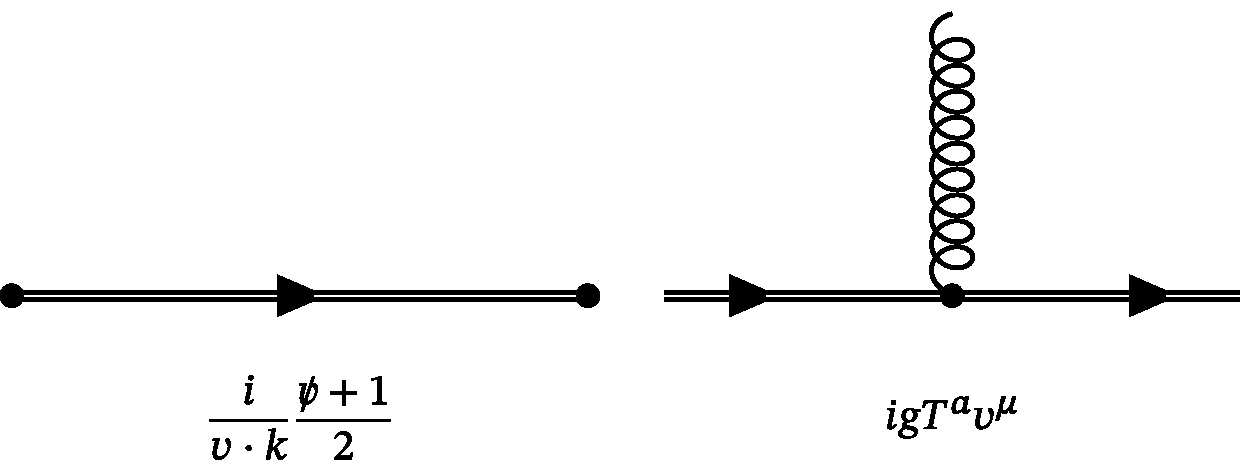
\includegraphics[width=0.8\textwidth]{figures/pdf/feynman_rules.pdf}
\caption{Feynman rules in HQET.}
\label{fig:hqet_feynman_rules}
\end{figure}

The Feynman rules of HQET (displayed in figure \ref{fig:hqet_feynman_rules}) are simpler than those of QCD and coincide with their HQ limit. For example, for the heavy quark propagator holds that
\begin{equation}
  \frac{i}{\slashed{P}_Q - m_Q} \to \frac{i}{v^\mu k_\mu} \frac{\slashed{v} + 1}{2} + \symcal{O}\left(\frac{k}{m_Q}\right) ,
\end{equation}
with $P_Q = m_Q v + k$, as $k / m_Q \to 0$. Also, the quark-gluon vertex simplifies, being evaluated between positive energy eigenstates 
\begin{equation}
  \operatorname{P}_+ \left( i g T^a \gamma^\mu \right) \operatorname{P}_+ = \operatorname{P}_+ \left( i g T^a v^\mu \right) \operatorname{P}_+ ,
\end{equation}
so that the vertex between a heavy quark and a gluon becomes simply $i g T^a v^\mu$, which does not contain gamma matrices.

It is important to observe that the HQET Lagrangian is not Lorentz invariant: under an infinitesimal transformation $\Lambda\indices{^\mu_\nu} = \delta\indices{^\mu_\nu} - i \omega\indices{^\mu_\nu}$ (acting on $h_v$ as $\operatorname{S} = \symbb{1} + \frac{i}{4} \omega_{\mu \nu} \sigma^{\mu \nu}$)
\begin{equation}
  \delta \symcal{L}_\text{HQET} = \omega\indices{^\mu_\nu} \adj{h}_v v_\mu D^\nu h_v ,
\end{equation}
indeed the selection of a particular four-velocity $v$ (i.e. a particular frame of reference, in which the heavy quark is at rest) breaks the Lorentz symmetry.

However, $\symcal{L}_\text{HQET}$ is invariant for transformations of $SU(2)$ acting on $h_v$ in the following way (for infinitesimal transformations)
\begin{equation}
  h_v \mapsto \left( 1 + i \symbf{\varepsilon} \cdot \symbf{S} \right) h_v ,
\end{equation}
which is the mathematical statement of the HQ spin symmetry of the HQET Lagrangian. Notice that these transformations preserve the positive energy condition indeed
\begin{equation}
  \operatorname{P}_+ \left( 1 + i \symbf{\varepsilon} \cdot \symbf{S} \right) h_v = \left( 1 + i \symbf{\varepsilon} \cdot \symbf{S} \right) h_v .
\end{equation}

It can be shown \cite{Mannel:1991mc} that, if one consider the full QCD Lagrangian and studies the case in which QCD interactions change the velocity of the heavy quark, in the limit $m_Q \to \infty$, the QCD Green functions involving one ingoing and one outgoing heavy quark vanish if the two velocity are different. This fact in the literature is sometimes referred to as \emph{velocity superselection rule}. Since there is no coupling among quarks with different velocities one can restore the Lorentz invariance of the HQET summing in a covariant way over the velocities (which, in this case, transform in turn covariantly). This generalization is due to Georgi \cite{Georgi:1990um} and the Lagrangian reads
\begin{equation}
  \symcal{L}_\text{HQET} = \int \! \frac{\D^3 \! v}{(2 \pi)^3} \frac{1}{2 \sqrt{\Vert \symbf{v} \Vert^2 + 1}} \; \adj{h}_v \left. i \ v^\mu D_\mu \right. h_v .
\end{equation}
It is easy to see that now $\symcal{L}_\text{HQET}$ is Lorentz-invariant, indeed for a finite transformation $\Lambda\indices{^\mu_\nu}$
\begin{multline}
  \symcal{L}_\text{HQET} = \int \! \frac{\D^4 \! v}{(2 \pi)^4} \; \delta^4 \! \left( v^2 - 1 \right) \, \theta ( v_0 ) \, \adj{h}_v \left. i \ v^\mu D_\mu \right. h_v \\ \mapsto \int \!  \frac{\D^4 \! u}{(2 \pi)^4} \; \vert \det{\Lambda} \vert \, \delta^4 \! \left( u^2 - 1 \right) \, \theta ( u_0 ) \, \adj{h}_u \left. i \ u^\mu D_\mu \right. h_u = \symcal{L}_\text{HQET} ,
\end{multline}
using the substitution $v = \Lambda u$ and taking into account that for a orthochronus Lorentz transformations holds $u_0 > 0$ and $\vert \det{\Lambda} \vert = 1$ .

\section{Spectroscopic Implications of HQET}
\label{sec:spectroscopic_implications_of_hqet}

The symmetries of HQET in the exact HQ limit provide a number of spectroscopic observable consequences:
\begin{itemize}
  \item for each hadronic state containing a heavy quark and for each flavour of the latter there is a degenerate doublet of states differing by the orientation of the heavy quark spin $\symbf{S}_Q$ and having the same full width;
  \item the sum of partial widths of strong decays between two doublets are the same for the two states of the initial doublet;
  \item the partial decay widths and mass splittings between different doublets are independent of the heavy quark flavour.
\end{itemize}

Moreover, due to the fact that, in the limit $m_Q \to \infty$, the heavy quark decouples from the LDoF, its spin $\symbf{S}_Q$ and the total angular momentum of LDoF $\symbf{S}_l$ are separately conserved. The total angular momentum of the LDoF's is the sum of the orbital angular momentum $\symbf{L}$ of the light quark with respect to the heavy quark and its spin $\symbf{S}_q$: $\symbf{S}_l = \symbf{L} + \symbf{S}_q$. However, it should be noticed that nothing prevents the existence of different states with the same values of $\symbf{S}_l$ and $\symbf{S}_Q$. These states are interpreted as \emph{radial excitations}, in analogy to non-relativistic systems (e.g. the hydrogen atom).

For the purpose of this work, from here on, I will concentrate on the heavy meson sector. Regarding the nomenclature for such particles, I will adhere to the convention of indicating the natural spin-parity series ($0^+, 1^-, 2^+, \cdots$) with an asterisk. We remember that the parity of a meson can be written as $P = (-1)^{L+1}$, having quarks and antiquarks opposite intrinsic parity. The spin of the particle will appear as a subscript, with the exception of the ground state with $S_\ell = (1/2)^-$, and the radial excitations will be indicated with a tilde.

In the ground state ($L = 0$) the quantum numbers of the LDoF's are those of the light antiquark, that is $S_\ell^P = (1/2)^-$. The corresponding doublet $(P, P^*)$ will contain a singlet state $P$ corresponding to a pseudoscalar particle with $J^P = 0^-$ and a triplet state $P^*$ corresponding to a vector one with $J^P = 1^-$. When $L =1$ two doublets can be built according to the two possible orientations of $\symbf{S}_q$. The doublet $(P_0^*, P_1)$ with $\symbf{S}_q$ antiparallel to $\symbf{L}$ will have the same angular momentum but opposite parity with respect to the ground state, that is $S_\ell = (1/2)^+$, and will contain a scalar $P_0^*$ with $J^P = 0^+$ and a pseudovector $P^\prime_1$ with $J^P = 1^+$. The other doublet $(P_1 , P_2^*)$, with $S_\ell^P = (3/2)^+$, will contain a axial particle $P_1$ with $J^P = 1^+$ and a tensor one $P_2^*$ with $J^P = 2^+$. In this way, doublets corresponding to higher values of $L$ can be analogously defined.

Let us consider the implications for the masses of these states. The ground state doublet is experimentally confirmed to be nearly degenerate both in the charm and beauty sector, with and without strangeness (within few percentage points of the mass of the state). Moreover, being the small mass splitting a relativistic correction of order $1/m_Q$, one can predict that $m^2_{D^*} - m^2_D \approx m^2_{B^*} - m^2_B$, which is also found to be true. For the same reason, one expects this relation to be true in the case of states with strangeness $m^2_{D_s^*} - m^2_{D_s} \approx m^2_{B_s^*} - m^2_{B_s}$. However, in principle, this quantity is not the same in the two cases, because the quantum numbers of the LDoF's are different. Nonetheless, the data shows that these are very similar and therefore it can be deduced that hyperfine corrections are approximately independent of the light quark flavour.

\section{Covariant Representation of Heavy Mesons}

As seen in section \ref{sec:et_general_remarks}, in non-decoupling effective theories fields with desired properties are introduced. These effective fields must belong to some representations of the symmetry group of the more fundamental theory in exam. However, these representations are in principle reducible and thus the effective fields can be decomposed in linear combinations of fields belonging to irreducible representations. Therefore, in general, effective fields represent multiplets of particles.

This is precisely the case of heavy mesons doublets. Because $\symbf{S}_Q$ and $\symbf{S}_l$ are separately conserved, as predicted by the HQET, the effective field $M$ must belong to the tensor product of the representations of $SO(3,1)$ to which belong the heavy quark and the LDoF's, i.e. the representation $ 2 \otimes \left( 2 \times S_\ell + 1 \right) =  2 \times S_\ell \oplus \left( 2 \times S_\ell + 2 \right)$.
Moreover, it must have the right parity, it must have one light and one heavy flavour indices and it must belong to the trivial representation of the $SU(3)_C$ group (because observable states are colour singlets).

% FIXME: riformulare 
%Finally, as another consequence of the HQET, there must be a frame of reference in which the heavy quark is at rest: the heavy meson effective field $M$ is built to have this property, i.e. in such a way that exist a meson energy projector $\operatorname{P}$ such that $\operatorname{P} M = M$. The frame of reference in which the meson is at rest is parametrized in the frame of reference of the laboratory by a four-velocity $v$.

Given a field $A_l$ with the quantum numbers of the LDoF's and a positive energy bispinor $\psi_h$ with those of the heavy quark, an effective field with the required properties is obtained by considering their tensorial product
\begin{equation}
  M_{h l} = \psi_h A_l .
\end{equation}
In the case of mesons $S_\ell$ is half-integer and therefore $A_l$ is a generalized Rarita-Schwinger vector-spinor transverse to $v$ \cite{Falk:1991nq}. The task of decomposing the effective fields in fields belonging to irreducible representations (and thus representing physical states) can be carried on in a general way \cite{Falk:1991nq}. As an illustrative example, in the following I describe this decomposition in the case of the ground state mesons.

%% <<================ REVIEW FROM HERE ===================>>
%% FIXME: prodotto tensoriale senza aggiunto di Dirac, perchè ce lo metto?
%In the ground state the LDoF's are represented by a bispinor $\psi_l$ which satisfy 
%\begin{equation}
%  \frac{1 - \slashed{v}}{2} \psi_l = \psi_l, \ \text{ hence } \; \adj{\psi_l} \; \frac{1 - \slashed{v}}{2} = \adj{\psi}_l
%\end{equation}
%and therefore the ground state meson doublet $H$ can be written as 
%\begin{equation}
%  H_{h l} = \psi_h \adj{\psi}_l ,
%\end{equation}
%which is a $4 \times 4$ complex matrix. However, $M$ has much less than $16 \times 2 = 32$ real DoF's. Indeed, $\psi_h$ and $\psi_l$ are respectively positive and negative energy bispinors, hence 
%\begin{equation}
%  H = \operatorname{P}_+ H \operatorname{P}_- = \frac{1 + \slashed{v}}{2} H \frac{1 - \slashed{v}}{2} .
%\end{equation}
%This condition in the rest frame reduces to the following (in the standard representation)
%\begin{equation}
%  M = \begin{pmatrix} 0 & A \\ 0 & 0 \end{pmatrix} ,
%\end{equation}
%where $A$ is a $2 \times 2$ complex matrix (8 real DoF's). But $A$ is obtained as the tensorial product of two normalized spinor
%\begin{equation}
%  \psi_h = \begin{pmatrix} \phi_h \\ 0 \end{pmatrix} , \qquad
%  \psi_l = \begin{pmatrix} 0 \\ \chi_l \end{pmatrix} , \qquad
%  M = \begin{pmatrix} 0 & - \phi_h \chi^\dagger_l \\ 0 & 0 \end{pmatrix} ,
%\end{equation}
%where $\phi_h$ and $\chi_l$ have just 2 real DoF's each (plus one irrelevant phase each). Therefore $H$ has $2 \times 2 = 4$ real DoF's, which is correct. This is because $M$ must belong to the representation $0 \oplus 1$, which means that it can be decomposed as the sum of two linearly independent vectors, each belonging to an invariant subspace with real dimension respectively $2 \times 0 + 1 = 1$ and $2 \times 1 + 1 = 3$.
%
%$H$ transforms with respect to Lorentz transformations with law
%\begin{equation}
%  H_{h l} = \operatorname{S} H_{h l} \adj{\operatorname{S}} ,
%\end{equation}
%where $S$ is a Lorentz transformation acting on bispinors.
%
%% <<================ REVIEW TO HERE ===================>>

In the case of the ground state, i.e. the doublet with $S_\ell^P = \left. 1/2 \right.^-$ ($P$ indicates parity), the LDoF's transform under the Lorentz group as an antiquark $\adj{\psi}_l$ satisfying
\begin{equation}
  \adj{\psi}_l \frac{1 - \slashed{v}}{2} = \adj{\psi}_l ,
\end{equation}
so that
\begin{equation}
  H = \psi_h \adj{\psi}_l .
\end{equation}
$H$ is a linear combination of objects with spin 0 and 1. The identification of these components is simpler in the rest frame where the spin operator is
\begin{equation}
  S^i = \frac{1}{2} \begin{pmatrix} \sigma^i & 0 \\ 0 & \sigma^i \end{pmatrix}
\end{equation}
and acts on $H$ in the following way
\begin{equation}
  \operatorname{\symbf{S}} H = \left( \operatorname{\symbf{S}} \psi_h \right) \adj{\psi}_l - \psi_h \left( \adj{\psi}_l \operatorname{\symbf{S}} \right) .
  \label{eq:spin_action_on_H}
\end{equation}
The basis of $H$ can be computed by definition as the tensorial product of the basis for $\psi_h$ and $\psi_l$. In the rest frame the vectors of these spinor basis are
\begin{equation}
  \Uparrow = \begin{pmatrix} 1 \\ 0 \\ 0 \\ 0 \end{pmatrix} , \quad
  \Downarrow = \begin{pmatrix} 0 \\ 1 \\ 0 \\ 0 \end{pmatrix} , \quad 
  \uparrow = \begin{pmatrix} 0 \\ 0 \\ 1 \\ 0 \end{pmatrix} , \quad 
  \downarrow = \begin{pmatrix} 0 \\ 0 \\ 0 \\ 1 \end{pmatrix} .
\end{equation}
Acting with $\symbf{S}$ on $\{ \left. i \otimes j  \, \right\vert \, i = \Uparrow, \Downarrow \, , \, \ j = \uparrow, \downarrow\}$ one finds that the linear combination
\begin{equation}
  \Uparrow \uparrow + \Downarrow \downarrow = \begin{pmatrix} 0 & - \symbb{1} \\ 0 & 0 \end{pmatrix}
\end{equation}
is invariant under transformations \eqref{eq:spin_action_on_H}, i.e. it is a basis of a one dimensional invariant subspace, and similarly
\begin{subequations}
  \begin{align}
    \Uparrow \downarrow + \Downarrow \uparrow &= \begin{pmatrix} 0 & \sigma^1 \\ 0 & 0 \end{pmatrix} , \\
    -i \left( \Uparrow \downarrow - \Downarrow \uparrow \right) &= \begin{pmatrix} 0 & \sigma^2 \\ 0 & 0 \end{pmatrix} , \\
    \Uparrow \uparrow - \Downarrow \downarrow &= \begin{pmatrix} 0 & \sigma^3 \\ 0 & 0 \end{pmatrix} , 
  \end{align}
\end{subequations}
is the basis of an invariant subspace of dimension three.

% TODO: check normalization and sign
Therefore in the rest frame the components of the ground state doublet can be written in the following way
\begin{subequations}
  \begin{align}
    P &= - \frac{1 + \gamma^0}{2} \gamma^5 ,\\
    P^{* i} &= \frac{1 + \gamma^0}{2} \gamma^i .
  \end{align}
\end{subequations}
Their expression can be boosted in a generic frame of reference and combined to give the expression of the ground state multiplet
\begin{equation}
  H =  \frac{1 + \slashed{v}}{2} \left( \left. P^* \right._\mu \gamma^\mu - P \gamma^5 \right)
  \label{eq:H_doublet}
\end{equation}
where $P^*$ is transverse to $v$ and the heavy and light flavour indices have been omitted.
% TODO: check normalization 
%Also notice that the prefactors $1/\sqrt{2}$ have been included in the definition of the fields and therefore have to be accounted for in the normalization of the latter. 

In the case of the first excited doublet $S$, with $S_\ell^P = (1/2)^+$, the decomposition can be carried on in a similar fashion and the expression of $S$ in terms of his axial and scalar component is 
\begin{equation}
  S = \frac{1 + \slashed{v}}{2} \left( \left. P^\prime_1 \right._\mu \gamma^\mu \gamma^5 - P^*_0 \right) .
  \label{eq:S_doublet}
\end{equation}

The expression of $H$ and $S$ shows the general property that doublets of opposite parity differ by a factor $\gamma^5$. Therefore, given the expression of a doublet with $L$ even and $S_\ell = L + 1/2$, the one with $L' = L + 1$ and $S_\ell = L' - 1/2$ can be obtained. The member of the multiplet with $L$ even and $S_\ell = L + 1$, that is $V$ with $J = L+1$ and $P$ with $J = L$, have the following form
\begin{subequations}
  \begin{align}
    V^{\mu_1 \cdots \mu_{L+1}} =& \frac{1 + \slashed{v}}{2} \epsilon\indices{_V^{\mu_1 \cdots \mu_L}_{\mu_{L+1}}} \gamma^{\mu_{L+1}} , \\
    P^{\mu_1 \cdots \mu_L} =& \frac{1 + \slashed{v}}{2} \gamma^5 \epsilon_P^{\nu_1 \cdots \nu_L} \sqrt{\frac{2 k + 1}{k + 1}} \left( \delta^{\mu_1}_{\nu_1} \cdots \delta^{\mu_L}_{\nu_L} - \frac{1}{2 L + 1} \gamma_{\nu_1} \left( \gamma^{\mu_1} - v^{\mu_1} \right) \delta^{\mu_2}_{\nu_2} \cdots \delta^{\mu_L}_{\nu_L} \right. \nonumber \\ 
    \phantom{P^{\mu_1 \cdots \mu_L} =} & \left. - \cdots - \frac{1}{2 L + 1} \delta^{\mu_1}_{\nu_1} \cdots \delta^{\mu_{L - 1}}_{\nu_{L - 1}} \left( \gamma^{\mu_L} - v^{\mu_L} \right) \right) ,
  \end{align}
\end{subequations}
where $\epsilon_V^{\mu_1 \cdots \mu_{L+1}}$ and $\epsilon_P^{\mu \cdots \mu_{L}}$ are polarization tensors.
\begin{table}
  \centering
  \begin{tabular}{c c c c c c c c c c c c c c}
    \toprule
    Doublet & &
      \multicolumn{2}{c}{$H$} & 
      \multicolumn{2}{c}{$S$} & 
      \multicolumn{2}{c}{$T$} & 
      \multicolumn{2}{c}{$X$} & 
      \multicolumn{2}{c}{$X'$} & 
      \multicolumn{2}{c}{$F$} \\
    \midrule
    \addlinespace
    $\left( L, S_\ell^P \right)$ & &
      \multicolumn{2}{c}{$\Bigg( 0, \left. \dfrac{1}{2} \right.^- \Bigg) $} & 
      \multicolumn{2}{c}{$\Bigg( 1, \left. \dfrac{1}{2} \right.^+ \Bigg) $} & 
      \multicolumn{2}{c}{$\Bigg( 1, \left. \dfrac{3}{2} \right.^+ \Bigg) $} & 
      \multicolumn{2}{c}{$\Bigg( 2, \left. \dfrac{3}{2} \right.^- \Bigg) $} & 
      \multicolumn{2}{c}{$\Bigg( 2, \left. \dfrac{5}{2} \right.^- \Bigg) $} & 
      \multicolumn{2}{c}{$\Bigg(  3, \left. \dfrac{5}{2} \right.^+ \Bigg) $} \\
    \addlinespace
    Mesons & & $P$ & $P^*$ & $P_0^*$ & $P'_1$ & $P_1$ & $P_2^*$ & $P_1^{* \prime}$ & $P_2$ & $P'_2$ & $P_3^*$ & $P_2^{* \prime}$ & $P_3$\\
    $J^P$ & & $0^-$ & $1^-$ & $0^+$ & $1^+$ & $1^+$ & $2^+$ & $1^-$ & $2^-$ & $2^-$ & $3^-$ & $2^+$ & $3^+$ \\
    \bottomrule
  \end{tabular}
  \caption{Nomenclature, spin and parity of the heavy meson doublets up to $S_\ell = 5/2$}
\end{table}

The meson doublets of both parities with $S_\ell$ equals to $1/2$, $3/2$ and $5/2$ are explicitly listed below, given their relevance within the research work presented in this thesis
\begin{subequations}
  \begin{align}
    T^\mu =& \frac{1+\slashed{v}}{2} \left( \left. P^*_2 \right.\indices{^\mu_\nu} \gamma^\nu - \left. P_1 \right._\nu \sqrt{\frac{3}{2}} \gamma^5 \left( \eta^{\mu \nu} - \frac{1}{3} \gamma^\nu \left( \gamma^\mu - v^\mu \right) \right) \right) \\
    X^\mu =& \frac{1+\slashed{v}}{2} \left( \left. P_2 \right.\indices{^\mu_\nu} \gamma^\nu \gamma^5 - \left. P^{* \prime}_1 \right._\nu \sqrt{\frac{3}{2}} \left( \eta^{\mu \nu} - \frac{1}{3} \gamma^\nu \left( \gamma^\mu + v^\mu \right) \right) \right) \\
    X^{\prime \mu \nu} =& \frac{1 + \slashed{v}}{2} \left( \left. P^*_3 \right.\indices{^{\mu \nu}_\rho} \gamma^\rho - \left. P^\prime_2 \right. \indices{_{\alpha \beta}} \sqrt{\frac{5}{3}} \gamma^5 \left( \eta^{\mu \alpha} \eta^{\nu \beta} - \frac{1}{5} \gamma^\alpha \eta^{\nu \beta} \left( \gamma^\mu - v^\mu \right) \right. \right. \nonumber \\
  \phantom{X^{\prime \mu \nu} =}& \left. \left. - \frac{1}{5} \gamma^\beta \eta^{\mu \alpha} \left( \gamma^\nu - v^\nu \right) \right) \vphantom{\sqrt{\frac{5}{3}}} \! \right) , \\
  F^{\mu \nu} =& \frac{1 + \slashed{v}}{2} \left( \left. P_3 \right.\indices{^{\mu \nu}_\rho} \gamma^\rho \gamma^5 - \left. P^{* \prime}_2 \right.\indices{_{\alpha \beta}} \sqrt{\frac{5}{3}} \left( \eta^{\mu \alpha} \eta^{\nu \beta} - \frac{1}{5} \gamma^\alpha \eta^{\nu \beta} \left( \gamma^\mu + v^\mu \right) \right. \right. \nonumber \\  
  \phantom{F^{\mu \nu} =}& \left. \left. - \frac{1}{5} \gamma^\beta \eta^{\mu \alpha} \left( \gamma^\nu + v^\nu \right) \right) \vphantom{\sqrt{\frac{5}{3}}} \! \right) . 
  \end{align}
  \label{eq:other_doublets}
\end{subequations}
Their content in terms of meson states is reported in table \ref{tab:quark_masses}. Moreover, for the same reason, I list below the formulas for the sum of polarization tensors of rank 1, 2 and 3
\begin{subequations}
  \begin{align}
    \sum_\lambda \epsilon^{(\lambda)}_\mu \epsilon^{* (\lambda)}_\nu =& - K_{\mu \nu} , \\
    \sum_\lambda \epsilon^{(\lambda)}_{\mu \nu} \epsilon^{* (\lambda)}_{\rho \sigma} =& \phantom{{}+{}} \frac{1}{2} K_{\mu \rho} K_{\nu \sigma} + \frac{1}{2} K_{\mu \sigma} K_{\nu \rho} - \frac{1}{3} K_{\mu \nu} K_{\rho \sigma} , \\
    \sum_\lambda \epsilon^{(\lambda)}_{\mu \nu \alpha} \epsilon^{* (\lambda)}_{\rho \sigma \beta} =&
    \phantom{{}+{}} \frac{1}{15} \left(K_{\mu \alpha} K_{\sigma \nu} + K_{\mu \sigma} K_{\alpha \nu} + K_{\mu \nu} K_{\alpha \sigma}\right) K_{\rho \beta} \nonumber \\
    \phantom{\sum_\lambda \epsilon^{(\lambda)}_{\mu \nu \alpha} \epsilon^{* (\lambda)}_{\rho \sigma \beta} =}&
    + \frac{1}{15} \left(K_{\mu \alpha} K_{\sigma \rho} + K_{\mu \sigma} K_{\alpha \rho} + K_{\mu \rho} K_{\alpha \sigma}\right) K_{\nu \beta} \nonumber \\
    \phantom{\sum_\lambda \epsilon^{(\lambda)}_{\mu \nu \alpha} \epsilon^{* (\lambda)}_{\rho \sigma \beta} =}&
    + \frac{1}{15} \left(K_{\mu \alpha} K_{\sigma \beta} + K_{\mu \sigma} K_{\alpha \beta} + K_{\mu \beta} K_{\alpha \sigma}\right) K_{\nu \rho} \nonumber \\
    \phantom{\sum_\lambda \epsilon^{(\lambda)}_{\mu \nu \alpha} \epsilon^{* (\lambda)}_{\rho \sigma \beta} =}&
    - \frac{1}{6}  \left( K_{\mu \nu} K_{\alpha \rho} + K_{\mu \rho} K_{\nu \alpha} \right) K_{\sigma \beta} \nonumber \\
    \phantom{\sum_\lambda \epsilon^{(\lambda)}_{\mu \nu \alpha} \epsilon^{* (\lambda)}_{\rho \sigma \beta} =}&
    - \frac{1}{6}  \left( K_{\mu \rho} K_{\alpha \beta} + K_{\mu \beta} K_{\rho \alpha} \right) K_{\sigma \nu} \nonumber \\
    \phantom{\sum_\lambda \epsilon^{(\lambda)}_{\mu \nu \alpha} \epsilon^{* (\lambda)}_{\rho \sigma \beta} =}&
    - \frac{1}{6}  \left(K_{\mu \nu} K_{\alpha \beta} + K_{\mu \beta} K_{\nu \alpha}\right) K_{\sigma \rho} ,
  \end{align}
  \label{eq:polarization_sums}
\end{subequations}
where
\begin{equation}
  K_{\mu \nu} = \eta_{\mu \nu} - v_\mu v_\nu .
\end{equation}

\section{Hadronic masses in HQET}

In the strict HQ limit, the two member $P$ and $P^*$ of the ground state doublet $H$ are exactly degenerate and their common mass can be written as
\begin{equation}
  m_H = \bar{\Lambda} + m_Q .
\end{equation}
Because $\bar{\Lambda}$ is independent of the heavy quark flavour, it can be interpreted as the mass of the LDoF's (in the ground state configuration). 

However, because the heavy quark masses are finite, the physical mass of $P$ and $P^*$ will obey an expansion of the form
\begin{equation}
  m - m_Q = \bar{\Lambda} + \frac{\Delta m^2}{2 m_Q} + \symcal{O}\left( \frac{1}{m^2_Q} \right) .
\end{equation}
The term of order $1/m_Q$ can be computed from
\begin{equation}
  \left\langle M \right. \left\vert M \right\rangle \Delta m^2 = - \left\langle M \right\vert \int \! \D^3 \! x \; \symcal{L}_1 (x) \left\vert M \right\rangle ,
\end{equation}
where $\symcal{L}_1$ is the first of the power corrections defined in \eqref{eq:hqet_power_corrections}. 

It can be shown that 
\begin{equation}
  \Delta m^2 \equiv - \lambda_1 - d \lambda_2 ,
  \label{eq:delta_m_hqet}
\end{equation}
where $\lambda_1$ and $\lambda_2$ are parameters equal for $P$ and $P^*$, representing the corrections respectively due to the kinetic and the chromo-magnetic operator, while $d$ is a dimensionless coefficient different for the two states. Notice that the term responsible for the mass splitting is chromo-magnetic one, parametrized by $\lambda_2$. Using the mass independent normalization of states
\begin{equation}
  \left\langle M (p') \right. \left\vert M(p) \right\rangle = \frac{2 p^0}{m_M} \left( 2 \pi \right)^3 \delta^3 \left( \symbf{p} - \symbf{p}' \right) ,
\end{equation}
it is found
\begin{equation}
  d_P = 3 , \quad d_{P^*} = -1 .
\end{equation}
Therefore, the relation \eqref{eq:delta_m_hqet} can be inverted, and in particular
\begin{equation}
  \lambda_2 = - \frac{1}{4} \left( \Delta m^2_{P^*} - \Delta m^2_P \right) \approx - \frac{1}{4} \left( m^2_{P^*} - m^2_P \right) .
\end{equation}

This considerations can be extended to all doublets. The mass splitting between the two members of a doublet is given by a term analogous to \eqref{eq:heavy_chromomagnetic_operator}. The mass splitting Lagrangian terms can be written as
\begin{multline}
  \symcal{L}_1 = \frac{1}{2 m_Q} \left( 
      \lambda_H \tr{\left( \adj{H}_a \sigma^{\mu \nu} H_a \sigma_{\mu \nu} \right)} 
    - \lambda_S \tr{\left( \adj{S}_a \sigma^{\mu \nu} S_a \sigma_{\mu \nu} \right)}
    + \lambda_T \tr{\left( \adj{T}^\alpha_a \sigma^{\mu \nu} T_{a \alpha} \sigma_{\mu \nu} \right)} 
    \right. \\ \left.
    - \lambda_X \tr{\left( \adj{X}^\alpha_a \sigma^{\mu \nu} X_{a \alpha} \sigma_{\mu \nu} \right)} 
    + \lambda_{X'} \tr{\left( \adj{X}^{\prime \alpha \beta}_a \sigma^{\mu \nu} X'_{a \alpha \beta} \sigma_{\mu \nu} \right)} 
    - \lambda_F \tr{\left( \adj{F}^{\prime \alpha \beta}_a \sigma^{\mu \nu} F_{a \alpha \beta} \sigma_{\mu \nu} \right)} 
  \right) ,
\end{multline}
where the Dirac adjoint $\adj{M}$ of a heavy meson doublet $M$ is defined
\begin{equation}
  \adj{M} = \gamma^0 M \gamma^0
\end{equation}
and the constants $\lambda$ are related to the hyperfine splitting of each doublet
\begin{subequations}
  \begin{align}
    \lambda_H &= \frac{1}{8} \left( m^2_{P^*} - m^2_P \right) , \\
    \lambda_S &= \frac{1}{8} \left( m^2_{P'_1} - m^2_{P^*_0} \right) , \\
    \lambda_T &= \frac{3}{16} \left( m^2_{P^*_2} - m^2_{P_1} \right) , \\
    \lambda_X &= \frac{3}{16} \left( m^2_{P_2} - m^2_{P^{* \prime}_1} \right) , \\
    \lambda_{X'} &= \frac{5}{24} \left( m^2_{P^*_3} - m^2_{P'_2} \right) , \\
    \lambda_F &= \frac{5}{24} \left( m^2_{P_3} - m^2_{P^{* \prime}_2} \right) .
  \end{align}
\end{subequations}

\section{Chiral Symmetry Breaking}

The Chiral Perturbation Theory (ChPT or $\chi$PT) is an effective theory of the non-decoupling type (for a review see \cite{Scherer:2002tk}), which means that the low energy behaviour of (the sector of) theory which it models is not related to the decoupling of some heavy DoF but rather to the change of the nature of the DoF's of such theory. This effective theory relies on symmetry considerations and in particular exploits the concept of \emph{spontaneous symmetry breaking}. Indeed, the ChPT can be seen as a systematic method for discussing the consequences of the approximate global flavour symmetries of QCD at low energies. 

%I begin with recalling the Noether theorem and its quantum equivalent. The Noether theorem establishes the existence of conserved currents (currents with vanishing four-divergence) for a classical field theory with continuous symmetries. More precisely, suppose that the Lagrangian $\symcal{L}(\phi_i, \partial \phi_i)$ is invariant with respect to a group of transformations of the fields $\phi_i$ with infinitesimal form
%\begin{equation}
%  \phi_i (x) \mapsto \phi^\prime_i (x) = \phi_i(x) + \delta \phi_i(x) = \phi_i(x) - i \epsilon^a F^a_i \left( \phi_j(x) \right) ,
%\end{equation}
%where $\epsilon^a$ are $n$ constant parameters of the transformation, then there are $n$ conserved currents 
%\begin{equation}
%  \delta \symcal{L} = \epsilon^a (x) \partial_\mu J^{a \mu} + \partial_\mu \epsilon^a (x) J^{a \mu} .
%\end{equation}
%
%This can be illustrated effectively with the method of Gell-Mann and Lévy. Suppose that the Lagrangian $\symcal{L}(\phi_i, \partial \phi_i)$ is invariant with respect to a group of transformations of the fields $\phi_i$ with infinitesimal form
%\begin{equation}

%\end{equation}
%where $\epsilon^a$ are the constant parameters of the transformation. Then the method of Gell-Mann and Lévy consist to promote such transformations to local ones, calculate the variation $\delta \symcal{L}$ and then set back them to local. It can be easily checked (using the equation of motion) that
%\begin{equation}
%  \delta \symcal{L} = \epsilon^a (x) \partial_\mu J^{a \mu} + \partial_\mu \epsilon^a (x) J^{a \mu}
%\end{equation}
%or equivalently that
%\begin{align}
%  J^{a \mu} & = \frac{\partial \symcal{L}}{\partial \left( \partial_\mu \epsilon^a \right)} &, \\
%  \partial_\mu J^{a \mu} & = \frac{\partial \symcal{L}}{\partial \epsilon^a} &.
%\end{align}
%where 
%\begin{equation}
%  J^{a \mu} = -i \frac{\partial \symcal{L}}{\partial \left( \partial_\mu \phi_i \right)} F^a_i ,
%\end{equation}
%Then we set $\epsilon = \text{const.}$, in this way we simultaneously obtained the expression of the current and the conservation law.

The masses of the light quarks ($d$, $u$ and $s$) are much smaller than those of the heavy quarks and of lightest hadronic states ($m_\rho \approx 770 \ \text{MeV}$) with the exclusion of the pseudoscalar octet ($\pi$, $K$, $\eta$). This suggests on one hand to treat separately the light quarks and on the other that the mechanism that gives mass to the pseudoscalar octet may be different from that of other states.

The fermionic part of the QCD Lagrangian for the light quarks is
\begin{equation}
  \symcal{L}_\text{light} = \sum_{f = d, u, s} \adj{q}_f \left( i \slashed{D} - m_f \right) q_f .
\end{equation}
However, in the light of previous considerations, the mass terms can be neglected and the Lagrangian becomes
\begin{equation}
  \symcal{L}_\text{light} = \sum_{f = d, u, s} \adj{q}_f \left( i \slashed{D} \right) q_f .
  \label{eq:chiral_qcd_lagrangian}
\end{equation}
Because of the relations
\begin{equation}
  \adj{q} \Gamma q = 
  \begin{cases}
    \adj{q}_R \Gamma q_R + \adj{q}_L \Gamma q_L & \Gamma \in \{ \gamma^\mu , \gamma^\mu \gamma^5 \} \\
    \adj{q}_R \Gamma q_L + \adj{q}_R \Gamma q_L & \Gamma \in \{ 1 , \gamma^5 , \sigma^{\mu \nu} \} 
  \end{cases} ,
\end{equation}
\begin{equation}
  q_R = P_R q , \quad q_L = P_L q ,
\end{equation}
the Lagrangian can be written explicitly in terms of the chiral components
\begin{equation}
  \symcal{L}_\text{light} = \sum_{f = d, u, s} \adj{q}_{R, f} \left( i \slashed{D} \right) q_{R, f} + \adj{q}_{L, f} \left( i \slashed{D} \right) q_{L, f} .
\end{equation}

This Lagrangian has a larger symmetry group than the full theory. In absence of the mass term, it is possible to rotate separately the two chiral components of the quarks in flavour space, leaving the Lagrangian invariant. These transformations are the generalizations of \eqref{eq:u1_chiral_transformations} to $SU(3)$ 
\begin{subequations}
  \begin{align}
    U_R \colon q & \mapsto e^{i \theta_R^a T^a} q , \\
    U_L \colon q & \mapsto e^{i \theta_L^a T^a} q ,
  \end{align}
\end{subequations}
where $T^a$ are the generators of $SU(3)$ in the fundamental representation. The new symmetry group is then $SU(3)_R \times SU(3)_L \times U(1)_R \times U(1)_L$. The transformations of $U(1)_R \times U(1)_L$ can be re-parametrized as phase rotations of the chiral components respectively by the same or opposite angle. This leads to $U(1)_V \times U(1)_A$. However the latter is a symmetry group only of the classical theory and is broken in the quantum case (the so-called \emph{chiral anomaly}). Therefore, ultimately the symmetry group of the light QCD Lagrangian, in the limit of massless quarks, is $SU(3)_R \times SU(3)_L \times U(1)_V$. 

The $U(1)_V$ symmetry results in baryon number conservation. The charges of $SU(3)_R$ and $SU(3)_L$ are respectively $Q^a_R$ and $Q^a_L$, which can be recombined in the same way as the vector and axial $U(1)$ charges. Therefore, the following ones can be defined
\begin{subequations}
  \begin{align}
    Q^a_V &= Q^a_R + Q^a_L , \\
    Q^a_A &= Q^a_R - Q^a_L .
  \end{align}
\end{subequations}
These charges commute with $H^0_\text{QCD}$, the Hamiltonian of the theory described by \eqref{eq:chiral_qcd_lagrangian}, and it can be shown that they have definite parity, i.e. the action of the parity operator $\operatorname{P}$ is
\begin{subequations}
  \begin{align}
    \operatorname{P} Q^a_V \operatorname{P}^{-1} &= Q^a_V , \\
    \operatorname{P} Q^a_A \operatorname{P}^{-1} &= - Q^a_A .
  \end{align}
\end{subequations}

From these premises, one would conclude that for any state of positive parity there must exist a degenerate state of negative parity (\emph{parity doubling}). Indeed, if $\left\vert i, + \right\rangle$ is a state with energy $E_i$ and positive parity, then $\left\vert i, - \right\rangle = Q^a_A \left\vert i, + \right\rangle$ is a state with the same energy and negative parity, as can be seen from the following
\begin{gather}
  H^0_\text{QCD} \left\vert i, - \right\rangle = H^0_\text{QCD} Q^a_A \left\vert i, + \right\rangle = Q^a_A H^0_\text{QCD} \left\vert i, + \right\rangle = E_i \left\vert E_i, - \right\rangle , \\
  \operatorname{P} \left\vert i, - \right\rangle = \operatorname{P} Q^a_A \operatorname{P}^{-1} \operatorname{P} \left\vert i, + \right\rangle = - \left\vert i, - \right\rangle .
\end{gather}
Finally such a state can be decomposed in terms of the members of the multiplet with energy $E_i$ and negative parity
\begin{equation}
  \left\vert i , - \right\rangle = Q^a_A \left\vert i, + \right\rangle = - (T^a)_{i j} \left\vert j , - \right\rangle .
  \label{eq:parity_doubling_multiplet}
\end{equation}
However, the low-energy hadronic spectrum does not contain a degenerate baryon octet of negative parity. Therefore, it must be concluded that there is an inconsistency in the previous arguments.

Indeed it was tacitly assumed in the equation \eqref{eq:parity_doubling_multiplet} that the ground state of QCD is annihilated by $Q^a_A$. Let be $a^\dagger_i$ and $b^\dagger_i$ creator operators of states with quantum numbers $i$ and respectively positive and negative parity. Also assume that $\left\vert i , + \right\rangle$ and $\left\vert i, - \right\rangle$ can be decomposed with respect to two bases of irreducible representations of $SU(3)_L \times SU(3)_R$ and that under $SU(3)_L \times SU(3)_R$ the creation operators are related by
\begin{equation}
  \left[ Q^a_A , a^\dagger_i \right] = - \left( T^a \right)_{i j} b^\dagger_j ,
\end{equation}
then
\begin{equation}
  Q^a_A \left\vert i , + \right\rangle = \left( \left[ Q^a_A , a^\dagger_i \right] + a^\dagger_i Q^a_A \right) \left\vert 0 \right\rangle = - \left( T^a \right)_{i j} b^\dagger_j \left\vert 0 \right\rangle .
\end{equation}
However, if the ground state is not annihilated by $Q^a_A$ then \eqref{eq:parity_doubling_multiplet} does no longer apply. In this case, the ground state is not invariant under the full symmetry group of the Lagrangian, that is the theory exhibits spontaneous symmetry breaking. In this scenario, given their small mass, the mesons of the pseudoscalar meson octet are the candidates for the Goldstone bosons of the chiral symmetry breaking.

In this regard, it is worthy recalling that a non-vanishing scalar quark condensate in the chiral limit is a sufficient (although not necessary) condition for spontaneous symmetry breaking \cite{Scherer:2002tk}. This can be interpreted as follows. Quarks and antiquarks have strong attractive interactions, and, if they are massless, the energy cost of creating a new quark-antiquark pair is small. Thus one expects that the vacuum of QCD in the chiral limit will contain a condensate of quark-antiquark pairs, that is the vacuum expectation value of the scalar operator $\adj{Q} Q$ is non-zero
\begin{equation}
  \left\langle 0 \right\vert \adj{Q} Q \left\vert 0 \right\rangle = \left\langle 0 \right\vert \adj{Q}_L Q_R + \adj{Q}_R Q_L \left\vert 0 \right\rangle \neq 0 .
\end{equation}
This scalar condensate is not invariant under chiral transformations, as it couples quark components with opposite chirality.

In the following, it will be shown, as an example, that the pions have indeed the right quantum numbers to be the Goldstone bosons of the chiral symmetry breaking of the isospin group $SU(2)$. This subgroup of the light flavour rotations does not involve the strange quark and hence the relevant part of the Lagrangian \eqref{eq:chiral_qcd_lagrangian} does not contain its contribution.

The currents associated with $SU(2)_V \times SU(2)_A \times U(1)_V$ are
\begin{subequations}
  \begin{align}
    j^\mu &= \adj{Q} \gamma^\mu Q , \\
    j^{a \mu}_V &= \adj{Q} \gamma^\mu \tau^a Q , \\ 
    j^{a \mu}_A &= \adj{Q} \gamma^\mu \gamma^5 \tau^a Q , 
  \end{align}
\end{subequations}
where $\tau^a = \sigma^a / 2, a = 1, 2, 3$ are the generators of $SU(2)$. If the pions are Goldstone bosons of the broken $SU(2)_A$ group, then it is possible to parametrize the matrix element of $j^{a \mu}_A$ between the vacuum and an on-shell pion by writing
\begin{equation}
  \left\langle 0 \right\vert j^{a \mu}_A (x) \left\vert \pi^b (p) \right\rangle = - i p^\mu f \delta^{a b} e^{- i p \cdot x} ,
  \label{eq:chiral_current_matrix_elem}
\end{equation}
where $f$ is a constant with the dimensions of a mass. The value of $f$ can be determined from the weak decay rate of the charged pions (for this reason, $f$ is referred to as the \emph{pion decay constant}). Contracting \eqref{eq:chiral_current_matrix_elem} with $p_\mu$ and using the conservation of the axial current, it is found that the pion is massless $p^2 = 0$, as expected for Goldstone bosons.

If the mass terms are restored in \eqref{eq:chiral_qcd_lagrangian}, then the chiral components become coupled and using
\begin{equation}
  i \slashed{D} Q = \symbf{m} Q , \text{ with } \symbf{m} = 
  \begin{pmatrix}
    m_u & 0 \\
    0 & m_d 
  \end{pmatrix} ,
\end{equation}
the non-vanishing four-divergence of $j^{a \mu}_A$ can be calculated.
\begin{equation}
  \partial_\mu j^{a \mu}_A = i \adj{Q} \left\{ \symbf{m}, \tau^a \right\} Q .
\end{equation}
Inserting this relation in \eqref{eq:chiral_current_matrix_elem} one finds
\begin{equation}
  \left\langle 0 \right\vert \partial_\mu j^{a \mu}_A (x) \left\vert \pi^b (p) \right\rangle = - p^2 f \delta^{a b} = \left\langle 0 \right\vert i \adj{Q} \left\{ \symbf{m}, \tau^a \right\} Q \left\vert \pi^b (p) \right\rangle .
\end{equation}
But the last expression is an invariant quantity times
\begin{equation}
  \tr{\left( \left\{ \symbf{m}, \tau^a \right\} \tau^b \right)} = \frac{1}{2} \delta^{a b} \left( m_u + m_d \right) ,
\end{equation}
therefore, the quark and the pion masses are related by
\begin{equation}
  m^2_\pi = \left( m_u + m_d \right) \frac{M^2}{f} ,
\end{equation}
which is the notorious Goldberg-Treiman relation, where $M^2$ is a constant with dimensions of a mass squared.

\section{Chiral Perturbation Theory}

In light of all the previous considerations, a candidate non-decoupling effective theory for interactions of hadrons containing light quarks should exhibit the symmetries of the chiral QCD Lagrangian \eqref{eq:chiral_qcd_lagrangian} and the spontaneous breaking of $SU(3)_A$. As a matter of fact, it is possible to formulate effective theories of such type. Historically, the first of these was the linear sigma model by Gell-Mann and Lévy (1960), which was formulated to describe the pion-nucleon interactions. However, the original model predicted the existence of a particle not confirmed experimentally and therefore it was generalized to the so-called non-linear sigma model, which involves only physical particles. In the following, a more general formalism due to Callan, Coleman, Wess and Zumino (CCWZ formalism, see \cite{Coleman:1969sm} and \cite{Callan:1969sn}) will be shown, which will lead directly to the non-linear sigma model and to the theory for heavy mesons used in this thesis \cite{Manohar:1995xr}.

As an example, the following Lagrangian can be considered
\begin{equation}
  \symcal{L}_{O(N)} = \frac{1}{2} \partial_\mu \symbf{\phi} \cdot \partial^\mu \symbf{\phi} - \lambda \left( \symbf{\phi} \cdot \symbf{\phi} - v^2 \right)^2 ,
  \label{eq:ON_lagrangian}
\end{equation}
where $\symbf{\phi}$ is a real $N$-component scalar field. This Lagrangian has a global $O(N)$ symmetry. However, the potential is such that there is a continuum of configurations with minimum energy, characterized by the condition $\Vert \symbf{\phi} \Vert = v$ (the so-called \emph{vacuum manifold}, which in this case is the $N-1$ dimensional sphere $S^{N-1}$). Therefore, the $O(N)$ symmetry is spontaneously broken into $O(N-1)$ and the number of Goldstone bosons will be $N(N-1)/2 - (N-1)(N-2)/2 = N-1$, i.e. the number of broken generators. 

The Goldstone bosons will correspond to perturbations within the vacuum manifold about a standard vacuum configuration $\symbf{v}$, which is chosen to be 
\begin{equation}
  \symbf{v} = \begin{pmatrix} 0 \\ 0 \\ \vdots \\ v \end{pmatrix} .
\end{equation}
For this reason, one would like to introduce a set of coordinates describing the local orientation of the vacuum. The local vacua are obtained from $v$ through $\Xi (x) \in O(N)$, hence a natural choice is 
\begin{equation}
  \symbf{\phi} (x) = \Xi (x) \symbf{v} .
  \label{eq:phi_from_xi}
\end{equation}
The general CCWZ prescription is to choose a set of broken generators $X^a$ and write $\Xi(x)$ in terms of them
\begin{equation}
  \Xi (x) = \exp{\left( i \pi^a(x) X^a \right)} .
\end{equation}
In the considered example, such a choice could be $ \{ J_1, \cdots, J_{N-1} \}$, i.e. the set of generators of rotations with respect to the first $N-1$ axes 
\begin{equation}
  \Xi (x) = \exp{\left( \sum_{i = 1}^{N-1} \pi^i(x) J_i \right)} .
  \label{eq:ON_xi}
\end{equation}

It can be checked by an explicit calculation that the fields $\pi^i(x)$ are massless modes of the theory described by the Lagrangian \eqref{eq:ON_lagrangian} and indeed (for small perturbations about the vacuum, neglecting radial excitations)
\begin{equation}
  \symcal{L}_{O(N)} = \frac{1}{2} v^2 \left( \partial_\mu e^{- i \sum_{i = 1}^{N-1} \pi^i(x) J^i} \partial^\mu e^{i \sum_{i = 1}^{N-1} \pi^i(x) J^i} \right)_{N N} .
  \label{eq:linear_sigma_kinetic_lagrangian}
\end{equation}

A general feature of Goldstone bosons, which is manifest in the Lagrangian \eqref{eq:linear_sigma_kinetic_lagrangian}, is the fact that they are derivatively coupled. Therefore, because the derivatives of the fields are proportional to the momentum of such particles, in the low energy limit the Goldstone bosons are weakly coupled. This fact has an intuitive interpretation: global transformations of the Goldstone boson fields cannot change the energy of the system and hence only their derivatives can contribute to the Lagrangian.

However, in the formulation of effective field theories the Lagrangian is not given but it is built a posteriori in a way such that it is invariant under a certain group of symmetries. Therefore, in such contexts, it is worth knowing how the Goldstone boson fields transform under the broken symmetry group.

Consider the equations \eqref{eq:ON_xi} and \eqref{eq:phi_from_xi}, the same configuration $\phi(x)$ can be obtained as 
\begin{equation}
  \phi(x) = \Xi (x) h (x) \symbf{v} ,
\end{equation}
where
\begin{equation}
  h = \begin{pmatrix} h'(x) & 0 \\ 0 & 1 \end{pmatrix} , \text{ with } h'(x) \in O(N-1) .
\end{equation}
This observation is relevant for non-constant fields. Given a global transformation $g \in O(N)$, the transformed configuration $g \phi(x)$ will be obtained from the standard vacuum through $\Xi'(x)$ such that 
\begin{equation}
  g \Xi(x) = \Xi'(x) h(x) ,
  \label{eq:ccwz_condition}
\end{equation}
for some (in general) non trivial $h(x)$. Therefore, the transformation law of $\Xi(x)$ is
\begin{equation}
  \Xi(x) \mapsto g \Xi (x) h^{-1}\left( g , \Xi (x) \right)
  \label{eq:ccwz_transformation_law}
\end{equation}

%It is always possible to rotate the vacuum to a standard direction, which will be chosen to be $\symbf{v} = v \, \hat{\symbf{v}} = (0, 0, \dots, v)$, and express the configuration of the field $\symbf{\phi}$ with respect to this particular choice of the vacuum. In the generalized \emph{polar coordinates} $\symbf{\phi}$ has the following expression
%\begin{equation}
%  \symbf{\phi} = \left( \rho + v \right) e^{i \pi^a X^a} \hat{\symbf{v}} ,
%  \label{eq:generalized_polar_coordinates}
%\end{equation}
%where $\{\left. X^a \, \right\vert a = 1, \cdots, N-1 \}$ are the broken generators and $\pi^a$ are transformation parameters. $\pi^a$ and $\rho$ are together new field variables, related to the old ones by linear transformations only in proximity of the vacuum.
%
%The Lagrangian can be expressed in terms of these new variables
%\begin{equation}
%  \symcal{L}_{O(N)} = \frac{1}{2} \partial_\mu \rho \partial^\mu \rho - \lambda \left( \rho^2 + 2 \rho v \right)^2 \frac{1}{2} \left( \rho + v \right)^2 \left( \partial_\mu e^{- i \pi^a X^a} \partial^\mu e^{- i \pi^a X^a} \right)_{N N}
%\end{equation}
%where $(\quad)_{N N}$ is the element of the $N$th row and $N$th column. At small energies compared to the radial excitation mass $\sqrt{8 \lambda} v$, the contributions to the Lagrangian of higher order in $\rho$ can be neglected. At the leading order the Lagrangian is
%\begin{equation}
%  \symcal{L}_{O(N)} = \frac{1}{2} v^2 \left( \partial_\mu e^{- i \pi^a X^a} \partial^\mu e^{i \pi^a X^a} \right)_{N N} .
%  \label{eq:linear_sigma_kinetic_lagrangian}
%\end{equation}
%
%A general feature of Goldstone bosons, which is manifest in the Lagrangian \eqref{eq:linear_sigma_kinetic_lagrangian}, is the fact that they are derivatively coupled. Therefore, because the derivatives are proportional to the momentum of such particles, in the low energy limit the Goldstone bosons are weakly coupled. This fact has an intuitive interpretation: global transformations of the Goldstone bosons cannot change the energy of the system and hence only their derivatives can contribute to the Lagrangian.
%
%The arguments for the Lagrangian \eqref{eq:ON_lagrangian} can be replicated in a general way for any other theory with spontaneous symmetry breaking. Consider a theory with symmetry group $G$ and let $\phi$ be the dynamical field variables. If the potential operator of the theory is $\hat{V}$, then the vacuum manifold $\Psi_0$ is 
%\begin{equation}
%  \Psi_0 = \left\{ \left\vert \left. \psi_0 \right\rangle \, \right\vert \, \left\langle \psi_0 \right\vert \hat{V} (\hat{\phi}) \left\vert \psi_0 \right\rangle \text{ is minimum } \right\} .
%\end{equation}
%At tree level, the vacua are in correspondence with classical field configurations, such that
%\begin{equation}
%  V ( \left\langle \psi_0 \right\vert \hat{\phi} \left\vert \psi_0 \right\rangle ) = \left\langle \psi_0 \right\vert \hat{V} (\hat{\phi}) \left\vert \psi_0 \right\rangle 
%\end{equation}
%and therefore the vacuum manifold could be also written as
%\begin{equation}
%  \Phi_0 = \left\{ \left. \phi_0 \, \right\vert \, V(\phi_0) \text{ is minimum } \right\} .
%\end{equation}
%For each vacua $\phi_0$ there exists a subgroup $H_{\phi_0}$ of $G$ which leaves $\phi_0$ invariant. These groups are one isomorphic to the other (all the vacua are equivalent) and related by some $g \in G$ such that
%\begin{equation}
%  H_{\phi'_0} = g H_{\phi_0} g^{-1}
%\end{equation}
%Therefore, exist a unique abstract group $H$ which leaves the elements of $\Phi_0$ invariants and is called the unbroken group. Moreover, $H$ is normal and it can be shown that the vacuum manifold is isomorphic to its quotient group with respect to $G$
%\begin{equation}
%  \Phi_0 \simeq G / H .
%\end{equation}
%
%For small perturbations about the vacuum, holds locally a relation similar to \eqref{eq:generalized_polar_coordinates}
%\begin{equation}
%  \phi(x) = \Xi(x) \phi_0 , 
%\end{equation}
%with $\Xi (x) \in G$. Using the latter relation, it is possible to parametrize the DoF's of the theory with some subset of elements of $G$. The CCWZ prescription is to choose a set of broken generators $X^a$ and define the new field variables $\Xi$ in terms of the latter
%\begin{equation}
%  \Xi (x) = e^{i \pi^a (x) X^a} .
%\end{equation}
%In this way the fields $\pi^a$ are in the right number and have the right transformation properties to be identified with the Goldstone bosons of the broken symmetry. 
% 
%The transformation law of $\Xi$ can be obtained from the one of $\phi$. With respect to a global transformation $g \in G$, $\Xi$ transforms into $\Xi'$ such that, for some non-trivial $h(x)$, 
%\begin{equation}
%  g \Xi = \Xi' h \implies \Xi \mapsto g \Xi (x) h^{-1} (x) = g \Xi (x) h^{-1}\left( g , \Xi (x) \right)
%  \label{eq:ccwz_transformation_law}
%\end{equation}
%so that 
%\begin{equation}
%  \phi' = g \Xi(x) \phi_0 = \Xi'(x) h(x) \phi_0 .
%\end{equation}

This formalism can be applied to the chiral limit of QCD. In this case, neglecting $U(1)_V$, the original symmetry group of the theory is $SU(3)_R \times SU(3)_L$, while the unbroken is $SU(3)_V$. In order to define $\Xi$ it is necessary to choose a basis of broken generators. There are two common choices in the literature, the $\xi$-basis and the $\Sigma$-basis. Consider, for the sake of the argument, the transformations $g \in SU(3)_R \times SU(3)_L$ and $h \in SU(3)_V$, which in the chiral representation have the form
\begin{subequations}
  \begin{align}
    g &= \begin{pmatrix} R & 0 \\ 0 & L \end{pmatrix} , \\
    h &= \begin{pmatrix} U & 0 \\ 0 & U \end{pmatrix} , 
    \label{eq:g_and_h_definitions}
  \end{align}
\end{subequations}
where $R$, $L$, and $U$ are $SU(3)$ transformations acting on light flavour indices.

\paragraph{The $\xi$-basis} In this case one chooses the usual basis of $SU(3)_A$, that is 
\begin{equation}
  X^a_\xi = T^a_R - T^a_L .
\end{equation}
In the chiral representation this generators are block-diagonal with respect to the spinorial indices, hence
\begin{equation}
  \Xi (x) = e^{i \pi^a_\xi X^a_\xi} = \exp{\begin{pmatrix} i \pi^a_\xi T^a & 0 \\ 0 & - i \pi^a_\xi T^a \end{pmatrix}} = \begin{pmatrix} \xi & 0 \\ 0 & \xi^\dagger \end{pmatrix} , \quad \xi = e^{i \pi^a_\xi T} ,
\end{equation}
where $T^a$ are the $SU(3)$ generators in the fundamental representation. In this case the transformation law \eqref{eq:ccwz_transformation_law} has the form
\begin{equation}
  \begin{pmatrix} \xi & 0 \\ 0 & \xi^\dagger \end{pmatrix} \mapsto
  \begin{pmatrix} R & 0 \\ 0 & L \end{pmatrix}
  \begin{pmatrix} \xi & 0 \\ 0 & \xi^\dagger \end{pmatrix} 
  \begin{pmatrix} U^{-1} & 0 \\ 0 & U^{-1} \end{pmatrix} ,
\end{equation}
which implies
\begin{subequations}
  \begin{align}
    \xi &\mapsto L \xi U^{-1} , \\
    \xi^\dagger &\mapsto R \xi^\dagger U^{-1} .
    \label{eq:xi_transformation_law}
  \end{align}
\end{subequations}
Therefore $U \left(\xi(x), R, L \right)$ must be the solution of
\begin{equation}
  L \xi U^{-1} = U \xi R^\dagger .
  \label{eq:xi-base_U_condition}
\end{equation}

\paragraph{The $\Sigma$-basis} In this case  
\begin{equation}
  X^a_\Sigma = T^a_R ,
\end{equation}
which leads to
\begin{equation}
  \Xi (x) = e^{i \pi^a_\Sigma X^a_\Sigma} = \exp{\begin{pmatrix} i \pi^a_\Sigma T^a & 0 \\ 0 & 0 \end{pmatrix}} = \begin{pmatrix} \Sigma & 0 \\ 0 & \symbb{1} \end{pmatrix} , \quad \Sigma = e^{i \pi^a_\Sigma T} .
\end{equation}
The transformation law  
\begin{equation}
  \begin{pmatrix} \Sigma & 0 \\ 0 & \symbb{1} \end{pmatrix} \mapsto
  \begin{pmatrix} R & 0 \\ 0 & L \end{pmatrix}
  \begin{pmatrix} \Sigma & 0 \\ 0 & \symbb{1} \end{pmatrix} 
  \begin{pmatrix} U^{-1} & 0 \\ 0 & U^{-1} \end{pmatrix} ,
\end{equation}
provides the transformation law for $\Sigma$
\begin{equation}
  \Sigma \mapsto L \Sigma U^{-1}  
\end{equation}
and the explicit condition $U = L$. Finally, one has
\begin{equation}
  \Sigma \mapsto R \Sigma L^\dagger .
\end{equation}

It should be noticed that the two definitions are related by
\begin{equation}
  \Sigma (x) = \xi^2 (x) .
\end{equation}

The Goldstone boson fields are dimensionless, as it is clear in \eqref{eq:ON_xi} in which they are angular variables. When one writes the Lagrangian of an effective theory it is convenient to to use fields which have natural dimension one (i.e. of a mass). The standard choice in ChPT is to use the following definitions
\begin{equation}
  \xi = e^{\frac{i}{f_\pi}\symcal{M}}, \quad \Sigma = e^{\frac{2 i}{f_\pi} \symcal{M}} ,
\end{equation}
where $f_\pi \approx 132 \ \text{MeV}$ is the pion decay constant and the matrix $\symcal{M}$ is defined as
\begin{equation}
  \symcal{M} = \pi^a T^a = 
  \begin{pmatrix}
    \frac{1}{\sqrt{2}} \pi^0 + \frac{1}{\sqrt{6}} \eta & \pi^+ & K^+ \\
    \pi^- & - \frac{1}{\sqrt{2}} \pi^0 +  \frac{1}{\sqrt{6}} \eta & K^0 \\
    K^- & \adj{K}^0 & - \sqrt{\frac{2}{3}} \eta
  \end{pmatrix} .
\end{equation}

\section{Heavy ChPT}
\label{sec:heavy_ChPT}

As a first example of application of ChPT to heavy meson spectroscopy (a theory also known as heavy ChPT), it will be reviewed the construction of the Lagrangian for the ground state doublet $H$ at the leading order. To begin with, it should be noted that terms of the form $\tr{\left( \Sigma \Sigma^\dagger \cdots \Sigma \Sigma^\dagger \right)}$ are invariant with respect to global transformations $\Sigma \mapsto R \Sigma L^\dagger$. However, because $\Sigma \Sigma^\dagger = \symbb{1}$, all of them are constant. Therefore, non-constant scalar functions of $\Sigma$ must contain its derivatives. This is coherent with the previous statement that Goldstone bosons are derivatively coupled. Imposing also the Lorentz and parity invariance one finds that the simplest term is
\begin{equation}
  \symcal{L}_{\Sigma, \, \text{kin}} = \frac{1}{8} f^2_\pi \tr{\left( \partial_\mu \Sigma \partial^\mu \Sigma^\dagger \right)} ,
  \label{eq:sigma_kinetic_lagrangian}
\end{equation}
where the trace is computed over the light flavour indices. The interpretation of the latter as the kinetic term for $\Sigma$ is confirmed by its expansion
\begin{equation}
  \symcal{L}_{\Sigma, \, \text{kin}} = \tr{\left( \partial_\mu \symcal{M} \partial^\mu \symcal{M} \right)} + \symcal{O} \left( \symcal{M}^3 \right),
\end{equation}
which at the leading order in $\symcal{M}$ reproduces the kinetic terms for the (massless limit of the) mesons of the pseudoscalar octet 
\begin{equation}
  \tr{\left( \partial_\mu \symcal{M} \partial^\mu \symcal{M} \right)} = \frac{1}{2} \partial_\mu \pi^0 \partial^\mu \pi^0 + \partial_\mu \pi^- \partial^\mu \pi^+ + \cdots .
\end{equation}

In order to include $H$ in the effective theory, one has to know how this field transforms under $SU(3)_R \times SU(3)_L$. The CCWZ prescription for $H$ is
\begin{equation}
  H \mapsto H h^\dagger ,
  \label{eq:h_transformation_law}
\end{equation}
where $h$ is defined in equation \eqref{eq:g_and_h_definitions} and $U$ is fixed by the equation \eqref{eq:xi-base_U_condition}, hence is a function of $R$, $L$ and $\xi (x)$. A candidate kinetic term must be quadratic in $H$ and invariant with respect to such transformations, as well as to parity and charge conjugation, Lorentz transformations, heavy spin rotations and rotations in light and heavy flavour space.

Consider the product $\adj{H} H$, it has two light flavour indices, two heavy flavour indices and two spinorial indices. Hence, it is possible to construct a scalar by taking the trace with respect to all these indices. However, because such a trace $\tr{\left(\adj{H} H \right)}$ is a constant, the simplest scalars that can be built using $H$ are
\begin{equation}
  \tr{\left( \adj{H} \gamma^\mu \partial_\mu H \right)} , \quad \tr{\left( \adj{H} \partial_\mu H \gamma^\mu \right)} .
  \label{eq:simplest_H_lagrangians}
\end{equation}
However, given the property
\begin{equation}
  \frac{1 + \slashed{v}}{2} H \frac{1 - \slashed{v}}{2} = H ,
  \label{eq:H_positive_energy}
\end{equation}
both the terms \eqref{eq:simplest_H_lagrangians} are found to be proportional to
\begin{equation}
  \symcal{L}_{H, \, \text{kin}} = \tr{\left( \adj{H} \left. i \ v^\mu \partial_\mu \right. H \right)} ,
  \label{eq:H_kinetic}
\end{equation}
which has all the required symmetries but the Lorentz one. Nonetheless, the latter can be made Lorentz invariant summing covariantly over four-velocities, like the HQET Lagrangian \eqref{eq:hqet_lagrangian}. Indeed, the Lorentz invariant generalization of \eqref{eq:H_kinetic} could be written by making explicit use of the \emph{velocity superselection rule} in the following way
\begin{equation}
  \symcal{L}_{H , \, \text{kin}} = \int \frac{1}{2 \sqrt{\Vert \symbf{v} \Vert^2 + 1}} \frac{\D^3 \! v}{(2 \pi)^3} \frac{1}{2 \sqrt{\Vert \symbf{v}' \Vert^2 + 1}} \frac{\D^3 \! v'}{(2 \pi)^3} \; \tr{\left(\adj{H}_v \left. i \ v^\mu D_\mu \right. H_{v'} \right)} \delta \left( \symbf{v}' - \symbf{v} \right) ,
\end{equation}
where $H_v$ is a doublet moving with velocity $v$. The latter equation can be understood as the trace with respect to the \emph{velocity index} and therefore in the following I will just write $\symcal{L}_{H, \, \text{kin}}$ as in \eqref{eq:H_kinetic}.

Finally an interaction term between $\pi^a$ and $H$ must be introduced, to this end it is convenient to introduce the definitions
\begin{subequations}
  \begin{align}
    A^\mu &= \frac{i}{2} \left( \xi \partial^\mu \xi^\dagger - \xi^\dagger \partial^\mu \xi \right) = \frac{1}{f_\pi} \partial^\mu \pi + \cdots , \\
    V^\mu &= \frac{1}{2} \left( \xi \partial^\mu \xi^\dagger + \xi^\dagger \partial^\mu \xi \right) = \frac{1}{2 f_\pi^2} \left[ \pi , \partial^\mu \pi \right] + \cdots .
  \end{align}
\end{subequations}
Using the latter and equation \eqref{eq:xi_transformation_law}, it can be shown that the transformation law of these two matrix fields are
\begin{subequations}
  \begin{align}
    A^\mu &\mapsto h A^\mu h^\dagger , \\
    V^\mu &\mapsto h V^\mu h^\dagger + h \partial^\mu h^\dagger ,
  \end{align}
\end{subequations}
where $h$ is the same appearing in \eqref{eq:h_transformation_law}. On one hand, this allows to define the covariant derivative
\begin{gather}
  D^\mu H = \partial^\mu H - H V^\mu , \\
  D^\mu H \mapsto D^\mu H h^\dagger ,
\end{gather}
and thus introduce an invariant interaction term with $V$ simply using the substitution 
\begin{equation}
  \tr{\left( \adj{H} \left. i \ v^\mu \partial_\mu \right. H \right)} \mapsto \tr{\left( \adj{H} \left. i \ v^\mu D_\mu \right.  H \right)} .
\end{equation}
On the other hand, it is possible to show that the simplest valid interaction term containing $A$ (which is axial) is
\begin{equation}
  \symcal{L}_\text{Int} = g \tr{\left( \adj{H} H \slashed{A} \gamma^5 \right)} ,
\end{equation}
where the trace is over the light, heavy and \emph{velocity} indices. Finally, it is possible to write the most general Lagrangian consistent with the required symmetries
\begin{equation}
  \symcal{L}_H = \tr{\left( \adj{H} \left. i \ v^\mu  D_\mu \right. H \right)} + \frac{1}{8} f^2_\pi \tr{\left( \partial_\mu \Sigma^\dagger \partial^\mu \Sigma \right)} + g \tr{\left( \adj{H} H \slashed{A} \gamma^5 \right)} .
  \label{eq:HChPT_ground_state_lagrangian}
\end{equation}

This kind of construction can be applied to all possible doublets and their radial excitations at any order. The result is a theory with many LEC's and the $S$-matrix of this theory to any given order possess all the symmetries of the chiral and heavy-quark limit of the QCD (see \ref{sec:et_general_remarks}). However, to any given process it will correspond a relevant part of the Lagrangian which will contain only a small number of terms. Because the decays towards the ground state doublet are kinematically favoured (and experimentally more easily accessible), in the following I will focus on the modes $M \to H \pi $, where $M$ is a member of a generic doublet, $\pi$ here indicates a generic light pseudoscalar meson and $H$ denotes a member of the fundamental doublet. At the leading order, such processes will be described by a vertex which couples directly $M$, $H$ and $\pi$. Therefore, the relevant part of the heavy ChPT Lagrangian will be similar to the last term in \ref{eq:HChPT_ground_state_lagrangian}. 

The kinetic terms for $M$ with $S_\ell^P = \left( k + 1 / 2 \right)^\pm$ are of the form
\begin{equation}
  \symcal{L}_{M \text{, kin}} = \tr{\left( \adj{M}^{\alpha_1 \cdots \alpha_k} \left( \left. i \ v^\mu D_\mu \right. - \Delta_M \right) M_{\alpha_1 \cdots \alpha_k} \right)} ,
\end{equation}
where the trace is performed over all free indices and $\Delta_M = \average{m}_M - \average{m}_H$ is the difference between the spin-averaged masses of $M$ and $H$, the so-called intra-doublet mass splitting. A particle with spin $J$ will have $2 J + 1$ polarization modes, therefore, because a doublet $M$ with $S_\ell = k + 1 / 2 $ will contain a state $P_k$ with spin $J = k$ and a state $P_{k + 1}$ with spin $J = k + 1$, the spin-averaged mass will be
\begin{equation}
  \average{m}_M = \frac{(2 k + 1) m_{P_k} + (2 k + 3) m_{P_{k + 1}}}{4 ( k + 1) } .
\end{equation}

There is not a general formula for the form of the interaction term(s) of $M$ with $H$, which has to be derived imposing the invariance under Lorentz transformations, parity and charge conjugation, heavy-spin rotations and separate heavy and light flavour rotations. However, it is found that mesons sharing the same $S_\ell$ have the same interaction term form, irrespectively of their parity. It should be noticed that it is not guaranteed that there exists only one form compatible with these symmetries, as in the the case of $S_\ell = 5/2$. If there is more than one interaction term, each one will have its coupling constant and will interfere coherently with the others. I list below the interaction terms forms up to $S_\ell = 5/2$
\begin{subequations}
  \begin{align}
    \symcal{L}_{1/2 \text{, Int}} \propto& \tr{\left( \adj{H} M \slashed{A} \gamma^5 \right)} + \text{h.c.} \ , \\
    \symcal{L}_{3/2 \text{, Int}} \propto& \frac{1}{\Lambda_\chi} \tr{\left( \adj{H} M^\mu \left( i \ D_\mu \slashed{A} + i \ \slashed{D} A_\mu \right) \gamma^5 \right)} + \text{ h.c. } \ , \\
    \symcal{L}^{(1)}_{5/2 \text{, Int}} \propto& \frac{1}{\Lambda_\chi^2} \tr{\left( \adj{H} M^{\mu \nu} \left( D_\mu D_\nu \slashed{A} + D_\nu D_\mu \slashed{A} \right) \gamma^5 \right)} + \text{ h.c. } \ , \\ 
    \symcal{L}^{(2)}_{5/2 \text{, Int}} \propto& \frac{1}{\Lambda_\chi^2} \tr{\left( \adj{H} M^{\mu \nu} \left( D_\mu \slashed{D} A_\nu + D_\nu \slashed{D} A_\mu \right) \gamma^5 \right)} + \text{ h.c. } \ ,
  \end{align}
  \label{eqs:HChPT_interaction_Lagrangians}
\end{subequations}
where $\Lambda_\chi \approx 1 \ \text{GeV}$ is the chiral symmetry breaking scale and appears for dimensional reasons.


% vim: ft=tex nonumber wrap linebreak display+=lastline guifont=Inconsolata\ 20 spell spelllang=en_gb

\chapter{Taxonomy of Charmed Mesons}

\epigraph{\textitalian{All'inizio, l'arte del puzzle sembra un'arte breve, di poco spessore, tutta contenuta in uno scarno insegnamento della \emph{Gestalttheorie}: l'oggetto preso di mira---sia esso un atto percettivo, un apprendimento, un sistema fisiologico o, nel nostro caso, un puzzle di legno---non è una somma di elementi che bisognerebbe dapprima isolare e analizzare, ma un insieme, una forma cioè, una struttura: l'elemento non preesiste all'insieme, non è più immediato ne più antico, non sono gli elementi a determinare l'insieme, ma l'insieme a determinare gli elementi: la conoscenza del tutto e delle sue leggi, dell'insieme e della sua struttura, non è deducibile dalla conoscenza delle singole parti che lo compongono: la qual cosa significa che si può guardare il pezzo di un puzzle per tre giorni di seguito credendo di sapere tutto della sua configurazione e del suo colore, senza aver fatto il minimo passo avanti: conta solo la possibilità di collegare quel pezzo ad altri pezzi e in questo senso l'arte del puzzle e l'arte del go hanno qualcosa in comune; solo i pezzi ricomposti assumeranno un carattere leggibile, acquisteranno un senso: isolato, il pezzo di un puzzle non significa niente; è semplicemente una domanda impossibile, sfida opaca; ma se appena riesci, dopo molti minuti di errori e tentativi, o in un mezzo secondo prodigiosamente ispirato, a connetterlo con uno dei pezzi vicini, ecco che quello sparisce, cessa di esistere in quanto pezzo: l'intensa difficoltà che ha preceduto l'accostamento e che la parola \emph{puzzle}---enigma---traduce così bene in inglese, non solo non ha più motivo di esistere, ma sembra non averne avuto mai, tanto si è fatta evidenza: i due pezzi miracolosamente riuniti sono diventati ormai uno, a sua volta fonte di errori, esitazioni, smarrimenti e attesa.}}{(George Perec, \emph{La Vie mode d'emploi})}

In the first chapter it was seen that different open-charm meson states and some open-beauty ones have been observed and, thanks to LHCb and BelleII, one expects that as time goes by these spectra will become more and more populated. In the second chapter it was introduced a theoretical framework inspired by QCD which on one hand allows to classify the heavy-light mesons and on the other to describe their low-energy strong interactions with light pseudoscalar mesons in terms of a small number of unknown constants (which in principle should be obtained in some other way, e.g. experimentally). In this chapter, such theory is used for the classification of established and recently observed open-charm mesons according to its scheme \cite{Colangelo:2012xi}. Moreover, the decay widths of these states (with respect to selected decay modes) will be calculated within this theory and it will be shown how the result can be used to make model-independent predictions of their quantum numbers.

\section{Strong Two-body decays to the Fundamental Doublet}

%\begin{table}
%  \centering
%  \begin{tabular}{c c c c c c c c}
%    \toprule
%    & & \multicolumn{2}{c}{$c \adj{q}$} & \multicolumn{2}{c}{$c \adj{s}$} & $b \adj{q}$ & $b \adj{s}$  \\
%    Doublet & $J^P$ & $n_r = 1$ & $n_r = 2$ & $n_r = 1$ & $n_r = 2$ & $n_r = 1$ & $n_r = 1$ \\
%    \midrule
%    $H$ & $0^-$ & $D(1869)$ & $\left. D(2550) \right.^\star$ & $D_s(1968)$ & & $ B(5279)$ & $ B_s(5366)$ \\ 
%    $H$ & $1^-$ & $D^*(2010)$ & $\left. D^* (2600) \right.^\star$ & $D_s^*(2112)$ & $D_{s1}^*(2700)$ & $ B^*(5325)$ & $ B_s^*(5415)$ \\
%    \addlinespace
%    $S$ & $0^+$ & $D^*_0(2400)$ & & $D_{s0}^*(2317)$ & & & \\
%    $S$ & $1^+$ & $D'_1(2430)$ & & $D'_{s1}(2460)$ & $\left. D_{sJ}(3040) \right.^\star$ & & \\
%    \addlinespace
%    $T$ & $1^+$ & $D_1(2420)$ & & $D_{s1}(2536)$ & $\left. D_{sJ}(3040) \right.^\star$ & $ B_1(5721)$ & $B_{s1}(5830)$ \\
%    $T$ & $2^+$ & $D^*_2(2460)$ & $\left. D^*_2(3000) \right.^\star$ & $D_{s2}^*(2573)$ & & $ B_2^*(5747)$ & $ B_{s2}^*(5840)$ \\
%    \addlinespace
%    $X$ & $1^-$ & & & $D^*_{s 1}(2860)$ & & & \\
%    $X$ & $2^-$ & & & & & & \\
%    \addlinespace
%    $X'$ & $2^-$ & $\left. D(2750) \right.^\star$ & & & & & \\
%    $X'$ & $3^-$ & $D^*_3(2760)$ & & $D^*_{s 3}(2860)$ & & & \\
%    \addlinespace
%    $F$ & $2^+$ & $\left. D^*_2(3000) \right.^\star$ & & & & & \\
%    \bottomrule
%  \end{tabular}
%  \caption{Observed open-charm and open-beauty mesons, classified in HQ doublets. States with uncertain assignment are indicated with $\star$.}
%  \label{tab:charm}
%\end{table}

I will recall some basic facts. The classification of heavy mesons is based on the quantum numbers of the light degrees of freedom (light quark plus gluons) and of the heavy quark, which decouples from the former due to its large mass. Therefore a state is characterized by the orbital angular momentum of the light degrees of freedom $L$, by their total angular momentum $S_\ell$ and by the meson spin $J$. Their parity will be $P = (-1)^{L + 1}$ and for each value of $S_\ell$ there will be two possible doublets of states with opposite parity, vice versa given $S_\ell^P$ there is only one possible value of $L$. The two states of each doublet are degenerate in the exact HQ limit, they correspond to the two possible orientations of the heavy meson spin and have different $J$. More than one state with any given combination of these quantum numbers can exist and accounts for radial excitations identified by increasing radial quantum number $n$.

In the first place, the classification of states is done according to their quantum number and mass, i.e. a resonance with given $J^P$ is a candidate for the lowest vacant states with that quantum numbers (which could have $n > 1$). However, apart for the $J = 0$ state, for each value of $J^P$ there exist two series of doublets, with respectively $S_l = \left( J - 1/2 \right)^P \text{ and } \left( J + 1/2 \right)^P$, that contain a state with the given $J^P$. To distinguish between these two series it is necessary to use an additional piece of information, which is carried by the width of the state.

As reviewed in section \ref{sec:heavy_ChPT}, in heavy ChPT it is possible to write effective Lagrangian terms that describe the strong decays of a heavy meson in a given doublet to another heavy meson in a second doublet with the emission of a light pseudoscalar meson. Eqs \ref{eqs:HChPT_interaction_Lagrangians} refer to the case in which the meson in the final state belongs to the fundamental doublet $H$. Each Lagrangian is weighted by a strong coupling constant that cannot be fixed within the same approach, so that it is in principle unknown. However, it should be stressed that a single parameter (i.e. the strong coupling constant) can describe (if allowed) four possible decays, corresponding to the two possible decaying mesons in the initial state doublet and two possible final state mesons in the other doublet. Therefore, such a parameter cancels in  the ratio of two strong decay rates computed from the same effective Lagrangian term. As a consequence, such ratios represent model independent predictions of the method.

Exploiting this approach, in the following I focus on the decays of a meson in a generic doublet $M$ to another one in the fundamental doublet $H$ with emission of a light pseudoscalar meson generically denoted as $\pi$. The reason of this lies in the large phase space available for these models and in the relative simplicity of their reconstruction in experimental analysis. The kinematics of the decays $M \to H \pi$ is that of a standard two body decay and its width can be written as
\begin{equation}
  \D \! \Gamma= \frac{1}{32 \pi^2} \left\vert \left\langle H \left( v \right), \pi \left( q \right) \right\vert T \left\vert M \left( v \right) \right\rangle \right\vert^2 \frac{\left\Vert \symbf{q} \right\Vert}{m_M} \D \! \Omega \ .
  \label{eq:diff_decay_width}
\end{equation}
%where $\symbf{p}'$ and $\epsilon$ are the momentum and polarization tensor of the daughter heavy meson, $\D \! \Omega$ is infinitesimal solid angle of around $\symbf{p}'$, $q$ is the four-momentum of the light pseudoscalar one and $v$, $\eta$ and $m_M$ are respectively the velocity, polarization and mass of the decaying heavy meson. At tree level holds
%\begin{equation}
%  \left\langle H \left( v , \epsilon \right), \pi \left( q \right) \right\vert S \left\vert M \left( v, \eta \right) \right\rangle = \left\langle H \left( v, \epsilon \right), \pi \left( q \right) \right\vert \symcal{L}_{M \text{, Int}} \left\vert M \left( v, \eta \right) \right\rangle \ ,
%\end{equation}
%where, with the normalization convention used, the $M(x)$ field is such that
%\begin{equation}
%  \left\langle 0 \right\vert M^{\mu_1 \cdots \mu_k}(x) \left\vert M(v , \epsilon) \right\rangle = \sqrt{m_M} \ \epsilon^{\mu_1 \cdots \mu_k} \ e^{- i v_\nu x^\nu} \ .
%\end{equation}
%
%Because one is interested in the unpolarized decay width, it is necessary to sum over the final polarization states and average over the initial ones. After these sums, using the relations \eqref{eq:polarization_sums}, the only four vector on which the RHS of the equation \eqref{eq:diff_decay_width} can depend are $v$ and $q$. Therefore, in the frame of reference in which the decaying heavy meson is at rest there is no preferred direction and the differential decay width of equation \eqref{eq:diff_decay_width} has no dependence on $\Omega$. Putting all together, it must be
%\begin{equation}
%  \Gamma= \frac{1}{16 \pi} \ \frac{1}{2 J + 1} \sum_\epsilon \sum_\eta \left\vert \left\langle H \left( v, \epsilon \right), \pi \left( q \right) \right\vert S \left\vert M \left( v , \eta \right) \right\rangle \right\vert^2 \frac{\left\Vert \symbf{p}' \right\Vert}{m_M} \ ,
%\end{equation}
%where $J$ is the spin of the decaying particle.

If the decaying meson has spin $J$ the factor $1/(2 J + 1)$ should be included in the equation \eqref{eq:diff_decay_width} to average over the spin.

$\left\langle H \left( v \right), \pi \left( q \right) \right\vert T \left\vert M \left( v \right) \right\rangle$ is the transition aplitude that can be directly computed from the effective Lagrangian terms. According to the velocity superselection rule, the two heavy mesons in the initial and final state have the same velocity. It is important to notice that this velocity superselection rule is valid only in the calculation of the matrix element and not in the calculation of the phase space that is fixed only by the kinematics.

In the frame of reference in which $M$ is at rest (i.e. $v = (1, \symbf{0})$) one has
\begin{equation}
  \left\Vert \symbf{q} \right\Vert = \frac{\sqrt{\left(m_M^2 - (m_H + m_\pi)^2\right) \left(m_M^2 - (m_H - m_\pi)^2\right)}}{2 m_M} .
\end{equation}

In the following I will list the allowed decays of heavy mesons belonging to one of the doublets introduced in equations \eqref{eq:H_doublet}, \eqref{eq:S_doublet}, \eqref{eq:other_doublets} and write down all the corresponding Lagrangian terms. Moreover, the covariant representation and structure of the interaction Lagrangian of states with $n > 1$ are the same as the corresponding one of the state with $n = 1$ and same $S_\ell^P$. However, the interaction Lagrangian terms for radial excited states have different coupling constants and, in the following, the coupling constant for the first radial excitation is denoted with the same symbol of the corresponding $n = 1$ state and marked by a tilde.

Some of the decay modes for $n = 2$ states of these mesons are explicitly listed in the following, because such decay modes towards doublets with higher $L$ are kinematically prohibited for $n = 1$ states but may be possible for ones with $n > 1$. Finally the Clebsh-Gordan coefficients associated with the light pseudoscalar meson in the final state (and built into the definition of $\symcal{M}$) are explicitly indicated with $C_\pi$.

It should be noticed that, the small $\Vert q \Vert$ behaviour of the decay widths reveal the dominant partial wave contribution to the decay and vice versa if the decay is known to occur in $l$-wave, at small $\Vert q \Vert$ will hold $\Gamma \propto \Vert q \Vert^{2 l+1}$.

\paragraph{Decaying meson $H = \left( P, P^* \right)$ or $\tilde{H} = \left( \tilde{P}, \tilde{P}^* \right)$}
\begin{equation}
  \symcal{L}_{H \text{, Int}} = g \tr{\left(\adj{H}_a H_b \gamma_\mu \gamma^5 A_{ba}^\mu \right)} \ .
\end{equation}
Allowed decays 
\begin{subequations}
  \begin{align}
    \Gamma \left( P^* \to P \pi \right) &= C_\pi \frac{g^2}{6 \pi f_\pi^2} \frac{m_P}{m_{P^*}} \left\Vert \symbf{q} \right\Vert^3 \ , \\
    \Gamma \left( \tilde{P}^* \to P \pi \right) &= C_\pi \frac{\tilde{g}^2}{6 \pi f_\pi^2} \frac{m_P}{m_{\tilde{P}^*}} \left\Vert \symbf{q} \right\Vert^3 \ , \\
    \Gamma \left( \tilde{P}^* \to P^* \pi \right) &= C_\pi \frac{\tilde{g}^2}{3 \pi f_\pi^2}\frac{m_{P^*}}{m_{\tilde{P}^*}} \left\Vert \symbf{q} \right\Vert^3 \ , \\
    \Gamma \left(\tilde{P} \to P^* \pi \right) &= C_\pi \frac{\tilde{g}^2}{2 \pi f_\pi^2} \frac{m_{P^*}}{m_{\tilde{P}}} \left\Vert \symbf{q} \right\Vert^3 \ .
  \end{align}
\end{subequations}

\paragraph{Decaying $S = \left( P^*_0, P'_1 \right)$}
\begin{equation}
  \symcal{L}_{S \text{, Int}} = h \tr{\left(\adj{H}_a S_b \gamma_\mu \gamma^5 A_{ba}^\mu \right)} + \text{h.c.} \ .
\end{equation}
Allowed decays
\begin{subequations}
  \begin{align}
    \Gamma \left( P^*_0 \to P \pi \right) &= C_\pi \frac{h^2}{2 \pi f_\pi^2} \frac{m_P}{m_{P^*_0}} \left\Vert \symbf{q} \right\Vert \left( m_\pi^2 + \left\Vert \symbf{q} \right\Vert^2 \right) \ , \\
    \Gamma \left( P'_1 \to P^* \pi \right) &= C_\pi \frac{h^2}{2 \pi f_\pi^2} \frac{m_{P^*}}{m_{P'_1}} \left\Vert \symbf{q} \right\Vert \left( m_\pi^2 + \left\Vert \symbf{q} \right\Vert^2 \right) \ .
  \end{align}
\end{subequations}

\paragraph{Decaying $T = \left( P_1, P^*_2 \right)$ or $\tilde{T} = \left(\tilde{P}_1, \tilde{P}^*_2 \right)$}
\begin{equation}
  \symcal{L}_{T \text{, Int}} =  \frac{h'}{\Lambda_\chi} \tr{\left(\adj{H}_a T^\mu_b \left( i D_\mu \slashed{A} + i \slashed{D} A_\mu \right)_{ba} \gamma^5 \right)} + \text{h.c.} \ .
\end{equation}
Allowed decays
\begin{subequations}
  \begin{align}
    \Gamma \left( P_1 \to P^* \pi \right) &= C_\pi \frac{2 h^{\prime 2}}{3 \pi f_\pi^2} \frac{m_{P^*}}{ m_{P_1}} \left\Vert \symbf{q} \right\Vert^5 \ , 
    \label{eq:P1toP*pi} \\
    \Gamma \left( P_2^* \to P \pi \right) &= C_\pi \frac{4 h^{\prime 2}}{15 \pi f_\pi^2} \frac{m_P}{m_{P_2^*}} \left\Vert \symbf{q} \right\Vert^5 \ , 
    \label{eq:P2*toPpi} \\
    \Gamma \left( P_2^* \to P^* \pi \right) &= C_\pi \frac{2 h^{\prime 2}}{5 \pi f_\pi^2} \frac{m_{P^*}}{m_{P_2^*}} \left\Vert \symbf{q} \right\Vert^5 \ .
    \label{eq:P2*toP*pi}
  \end{align}
\end{subequations}

\paragraph{Decaying $X = \left( P_1^* , P_2 \right)$}
\begin{equation}
  \symcal{L}_{X \text{, Int}} = \frac{k'}{\Lambda_\chi} \tr{\left( \adj{H}_a X^\mu_b \left( i D_\mu \slashed{A} + i \slashed{D} A_\mu \right)_{ba} \gamma^5 \right)} + \text{h.c.} \ .
\end{equation}
Allowed decays
\begin{subequations}
  \begin{align}
    \Gamma \left( P^*_1 \to P \pi \right) &= C_\pi \frac{4 k^{\prime 2}}{9 \pi f_\pi^2} \frac{m_P}{m_{P^*_1}} \left\Vert \symbf{q} \right\Vert^3 \left( m_\pi^2 + \left\Vert \symbf{q} \right\Vert^2 \right) \ , \\
    \Gamma \left( P^*_1 \to P^* \pi \right) &= C_\pi \frac{2 k^{\prime 2 }}{9 \pi f_\pi^2} \frac{m_{P^*}}{m_{P^*_1}} \left\Vert \symbf{q} \right\Vert^3 \left( m_\pi^2 + \left\Vert \symbf{q} \right\Vert^2 \right) \ , \\
    \Gamma \left( P_2 \to P^* \pi \right) &= C_\pi \frac{2 k^{\prime 2}}{3 \pi f_\pi^2} \frac{m_{P^*}}{m_{P_2}} \left\Vert \symbf{q} \right\Vert^3 \left( m_\pi^2 + \left\Vert \symbf{q} \right\Vert^2 \right) \ . \\
  \end{align}
\end{subequations}

\paragraph{Decaying $X' = \left( P_2, P^*_3 \right)$}
\begin{multline}
  \symcal{L}_{X' \text{, Int}} =  \frac{1}{\Lambda_\chi^2} \tr \left( \adj{H}_a X^{\prime \mu \nu}_b \left( k_1 \left( D_\mu D_\nu A_\lambda + D_\nu D_\mu A_\lambda \right) \right. \right. \\ +  \left. \left. k_2 \left( D_\mu D_\lambda A_\nu + D_\nu D_\lambda A_\mu \right) \right)_{ba}  \gamma^\lambda \gamma^5 \right) + \text{h.c.} \ .
\end{multline}
Allowed decays
\begin{subequations}
  \begin{align}
    \Gamma \left( P_2 \to P^* \pi \right) &= C_\pi \frac{4 k^2}{15 \pi f_\pi^2} \frac{m_{P^*}}{m_{P_2^{\prime *}}} \left\Vert \symbf{q} \right\Vert^7 \ , \\
    \Gamma \left( P^*_3 \to P \pi \right) &= C_\pi \frac{4 k^2}{35}{f_\pi^2} \frac{m_{P}}{m_{P^*_3}} \left\Vert \symbf{q} \right\Vert^7 \ , \\
    \Gamma \left( P^*_3 \to P^* \pi \right) &= C_\pi \frac{16 k^2}{105 \pi f_\pi^2} \frac{m_{P^*}}{m_{P^*_3}} \left\Vert \symbf{q} \right\Vert^7 \ ,
  \end{align}
\end{subequations}
with $k = k_1 + k_2$.

\paragraph{Decaying $F = \left( P^{* \prime}_2, P_3 \right)$}
\begin{multline}
  \symcal{L}_{F \text{, Int}} =  \frac{1}{\Lambda_\chi^2} \tr \left( \adj{H}_a F^{\mu \nu}_b \left( l_1 \left( D_\mu D_\nu A_\lambda + D_\nu D_\mu A_\lambda \right) \right. \right. \\ +  \left. \left. l_2 \left( D_\mu D_\lambda A_\nu + D_\nu D_\lambda A_\mu \right) \right)_{ba}  \gamma^\lambda \gamma^5 \right) + \text{h.c.} \ .
  \label{eq:F_Lagrangian}
\end{multline}
Allowed decays
\begin{subequations}
  \begin{align}
    \Gamma\left( P_2^{* \prime} \to P \pi \right) &= C_\pi \frac{4 l^2}{25 \pi f_\pi^2 \Lambda_\chi^4} \frac{m_P}{m_{P_2^{* \prime}}} \Vert \symbf{q} \Vert^5 \left( m^2_\pi + \Vert \symbf{q} \Vert^2 \right) \ , 
    \label{eq:P2*'toPpi} \\
    \Gamma\left( P_2^{* \prime} \to P^* \pi \right) &= C_\pi \frac{8 l^2}{75 \pi f_\pi^2 \Lambda_\chi^4} \frac{m_P^*}{m_{P_2^{* \prime}}} \Vert \symbf{q} \Vert^5 \left( m^2_\pi + \Vert \symbf{q} \Vert^2 \right) \ , 
    \label{eq:P2*'toP*pi} \\
    \Gamma\left( P_3 \to P^* \pi \right) &= C_\pi \frac{4 l^2}{105 \pi  f_\pi^2 \Lambda_\chi^4} \frac{m_{P^*}}{m_{P_3}} \left\Vert \symbf{q} \right\Vert^5 \left( 7 m_\pi^2 + 4 \left\Vert \symbf{q} \right\Vert^2 \right) \ ,
    \label{eq:P3toP*pi}
  \end{align}
\end{subequations}
with $l = l_1 + l_2$.

\section{Classification of Established States}

The established states of the open-charm meson spectrum are listed in table \ref{tab:charm_taxonomy} (together with the recently observed ones according to the classification proposed in this thesis) and, to give a bird's eye view, one could say that these states fill the $H$, $S$ and $T$ doublets. In the following I give an overview of their classification in some detail.

%The two states belonging to the fundamental doublet, with $S_\ell^P = 1/2^-$ and $n = 1$, are well known, both in the strange and non-strange sector (actually, the same is true for the open-beauty spectrum): the fundamental state is by definition the lightest $D_{(s)}$ meson and have $J^P = 0^-$ , the $D^*_{(s)}$ is the lightest $J^P = 1^-$ meson and decay through $p$-wave to $D_{(s)}$, all of their properties are in accord with the quark model for both neutral (without strangeness) and charged (with and without strangeness) versions. Therefore, this discussion will mainly concern the excited doublets with $S_\ell^P = \left. 1/2 \right.^+ , \left. 3/2 \right.^-, \cdots$ and/or $n > 1$. 

The fundamental doublet with $S_\ell^P = 1/2^-$ and $n = 1$ is filled by the well known states both in the strange and non-strange sector: the lightest $D_{(s)}$ meson with $J^P = 0^-$ and the $D^*_{(s)}$ meson with $J^P = 1^-$ meson; their properties are in agreement with quark model for both neutral and charges states.

If one looks at the observations of the open-charm and open-beauty states from a historical perspective, it is easy to spot a pattern in which states of the $T$ doublet are the first to be observed after the fundamental ones. This should cause no surprise: although the states of the $S$ doublet are lighter than those of the $T$ doublet (as expected by the quark model), the former have broad widths since they decay through $s$-wave and therefore they are more difficult to observe than the latter, which decay through $d$-wave and thus are rather narrow. Indeed, the $S_\ell^P = \left. 3/2 \right.^+$ states with $J^P = 1^+ \text{ and } 2^+$ are filled respectively by the $D_1(2420)$ and the $D^*_2(2460)$ in the non-strange sector and by the $D_{s1}(2536)$ and by the $D^*_{s 2}(2573)$ in the strange one.

The non-strange states with $S_\ell^P = \left. 1/2 \right.^+$ and $n = 1$ and are filled by the $D^*_0(2400)$ and by the $D'_1(2430)$, which have large widths and are the lightest known states with respectively $J^P = 0^+ \text{ and } 1^+$. Notice that the masses of the four states of both the $S$ and $T$ doublets lie in a range of about $100 \ \text{MeV}$, which is small compared to the splitting with respect to the $H$ doublet ($\approx 350 \ \text{MeV}$): this can be justified in light of the quark model because the $S$ and $T$ doublets have both $L = 1$ while $H$ has $L = 0$.

The case of charmed mesons with strangeness is more convoluted. As noticed in the first chapter, the mass of the $D^*_0(2317)$ and of the $D'_1(2460)$ are much smaller than suggested by the quark model for this doublet. This led to the speculation that these states may contain four quarks, either as tetraquark or as molecule formed by $D$ and $K$ mesons. The tetraquark picture predicts a large number of states, which were not observed by further search of the \textsc{BaBar} and Belle collaborations in the mass region of the $D^*_{s 0}$, hence making this picture disfavoured. Moreover, the masses of the $D^*_{s 0}$ and the $D_{s 1}$ are just below the threshold of $D K$ and $D^* K$ respectively, which accounts for the small widths of these states (unexpected for $S$ doublet states) since they are forced to decay violating isospin. This has suggested that these two states could be hadronic molecules or mixtures of hadronic molecules and ordinary $c \adj{s}$ mesons. However, theoretical predictions for their (isospin violating) hadronic and radiative decays \cite{Colangelo:2003vg,Colangelo:2005hv} strongly support their identification with the ordinary $c \adj{s}$ mesons belonging to the $S$ doublet.

The only remaining established state without strangeness is the $D^*_3(2760)$, also known as $D^*(2760)$ or $D(2750)$ in the PDG nomenclature. This state was known to have natural parity since its observation by \textsc{BaBar} (it decays to $D \pi$) and its spin-parity was later fixed by LHCb. Possible states with $J^P = 3^-$ and $n = 1$ are those belonging to $X'$ doublet, which has $L = 2$, and to a higher doublet with $L = 4$ (not considered in this thesis); however,the latter is expected to have much larger mass and so the $D^*_3(2760)$ is reasonably identified with the former.

The $D_{s J}(2860)$ and $D^*_{s 1}(2700)$ were observed both in the $D K$ and $D^* K$ channels by Belle and \textsc{BaBar} and later confirmed by LHCb. The spin-parity of $D^*_{s 1}(2700)$ was established by production studies, finding $J^P = 1^-$. Measurements of branching ratios and criteria based on heavy ChPT (analogous to those object of this thesis) suggested the identification with the $\tilde{D}^*_{s 1}$ \cite{Colangelo:2007ds}, the first radial excitation of the $D^*_s(2112)$. 

The common history of the $D^*_{s 1}(2860)$ and the $D^*_{s 3}(2860)$ dates back to an observation by the \textsc{BaBar} collaboration, indicated as the $D_{s J}(2860)$, the identification of which constituted a puzzle \cite{Colangelo:2012xi}. In \cite{Colangelo:2006rq} the identification of the $D^*_{s 3}(2860)$ with the state having $J^P = 3^-$ belonging to the $X'$ was proposed and later confirmed by LHCb \cite{Aaij:2014xza}. After that, $D^*_3(2760)$ was recognized as the non-strange partner of the $D^*_{s 3}(2860)$. The case of the $D^*_{s 1}(2860)$ is more uncertain and therefore is postponed in the following paragraph.

%\begin{table}
%  \centering
%  \small
%  \begin{tabular}{c c c c c c}
%    \toprule
%     & & & & \multicolumn{2}{c}{World averages} \\ 
%    \textsc{BaBar} (2010) & LHCb (2013) & LHCb (2016) & PDG & mass (MeV) & $\Gamma$ (MeV) \\ 
%    \midrule
%    $D(2550)$ & $D_J(2580)$ & & $D(2550)$ & $2564 \pm 20$  & $135 \pm 17$ \\
%    $D^*(2600)$ & $D^*_J(2650)$ & & $D^*_J(2600)$ & $2623 \pm 12$ & $139 \pm 31$ \\
%    $D^*(2760)$ & $D^*_J(2760)$ & & $D(2750)$ & $2763.5 \pm 3.4$ & $66 \pm 5$ \\
%    \bottomrule
%  \end{tabular}
%  \caption{Matching of nonestablished open-charm mesons by PDG.}
%  \label{tab:LHCb2013}
%\end{table}

\begin{table}
  \centering
  \footnotesize
  \begin{tabular}{c c c c c c c c}
    \toprule
    & & \multicolumn{3}{c}{$c \adj{q}$} & \multicolumn{3}{c}{$c \adj{s}$} \\
    Doublet & $J^P$ & $n = 1$ & $n = 2$ & $n = 3$ & $n = 1$ & $n = 2$ & $n = 3$ \\
    \midrule
    $H$ & $0^-$ & $D(1869)$ & $\left. D(2550) \right.^\star$ & & $D_s(1968)$ & & \\ 
    $H$ & $1^-$ & $D^*(2010)$ & $\left. D^* (2600) \right.^\star$ & $\left. D^*_1(2680) \right.^\star$ & $D_s^*(2112)$ & $D_{s1}^*(2700)$ & $\left. D^*_{s 1}(2860) \right.^\star$ \\
    \addlinespace
    $S$ & $0^+$ & $D^*_0(2400)$ & & & $D_{s0}^*(2317)$ & & \\
    $S$ & $1^+$ & $D'_1(2430)$ & $\left. D(3000) \right.^\star$ & & $D'_{s1}(2460)$ & $\left. D_{sJ}(3040) \right.^\star$ & \\
    \addlinespace
    $T$ & $1^+$ & $D_1(2420)$ & $\left. D(3000) \right.^\star$ & & $D_{s1}(2536)$ & $\left. D_{sJ}(3040) \right.^\star$ & \\
    $T$ & $2^+$ & $D^*_2(2460)$ & & & $D_{s2}^*(2573)$ & & \\
    \addlinespace
    $X$ & $1^-$ & $\left. D^*_1(2680) \right.^\star$ & & & $\left. D^*_{s 1}(2860) \right.^\star$ & & \\
    $X$ & $2^-$ & & & & & & \\
    \addlinespace
    $X'$ & $2^-$ & $\left. D(2750) \right.^\star$ & & & & & \\
    $X'$ & $3^-$ & $D^*_3(2760)$ & & & $D^*_{s 3}(2860)$ & & \\
    \addlinespace
    $F$ & $2^+$ & $\left. D^*_2(3000) \right.^\star$ & & & & & \\
    $F$ & $3^+$ & & & & & & \\
    \bottomrule
  \end{tabular}
  \caption{Observed open-charm mesons, classified in HQ doublets. States with uncertain identification are indicated with $\star$.}
  \label{tab:charm_taxonomy}
\end{table}

\section{Discussion of States of Uncertain Classification}

At present, the non-strange states with uncertain classification are the $D(2550)$ \cite{delAmoSanchez:2010vq,Aaij:2013sza}, the $D^*(2600)$ \cite{delAmoSanchez:2010vq}, the $D^*_J(2650)$ \cite{Aaij:2013sza,Aaij:2016fma}, the $D(2750)$ \cite{delAmoSanchez:2010vq}, the $D(3000)$ \cite{Aaij:2013sza} and the $D^*_2(3000)$ \cite{Aaij:2013sza,Aaij:2016fma}; while the strange ones are the $D^*_{s 1}(2860)$ \cite{Aaij:2014xza} and $D^*_{s J}(3040)$ \cite{Aubert:2009wg}.

\subsection{State Classification Discussed in the Literature}

As of their first observation, the \textsc{BaBar} collaboration suggested that the $D(2550)$ and the $D^*(2600)$ could belong to the $\tilde{H}$ doublet, i.e. with $S^P_\ell = \left. 1/2 \right.^-$ and $n = 2$, respectively with $J^P = 0^+$ and $1^-$. Hence these states are likely to be identified with the first radial excitations of $(D,\ D^*)$. The $D(2750)$ is regarded as the spin partner of the $D^*(2760)$, thus having $J^P = 2^-$. Comparison with quark model results corroborates these identifications (for a discussion see \cite{Colangelo:2012xi}).

The decay of $D_{sJ}(3040)$ to DK has not been observed, therefore unnatural parity assignment is highly favoured. The lightest not yet observed states of this series are the two $J^P = 2^-$ states with $L = 2$ and $n = 1$, the $3^+$ of the $F$ doublet and the two $J^P = 1^+$ states with $L = 1$ and $n = 2$. The two $2^-$ states are expected to be broader, while the $3^+$ to be heavier. Therefore the $D_{s J}(3040)$ is one of the two axial mesons\footnote{Since this particle has such a large, several decay modes are possible. In particular to decays to $D K^*$ and $D_s \phi$ should allow to discriminate between the $\tilde{D}_{s 1}$ and the $\tilde{D}'_{s 1}$, since the corresponding branching ratios are larger for the latter.} \cite{Colangelo:2010te}.

\subsection{State Classification Proposed in this Thesis}

The remaining states still requiring identification are those observed by LHCb in 2013 \cite{Aaij:2013sza} and 2016 \cite{Aaij:2016fma}. Among the latter, the $D_3^*(2760)$ can be identified with one of the previous observations, indeed it has the same $J^P$ of the $D(2750)$ (using the PDG nomenclature) and compatible mass and width, so it is excluded from further considerations. On the other hand, the identification of the $D(3000)$, $D_1^*(2680)$ and $D_2^*(3000)$ is uncertain. In the remaining of this section I propose a classification of these mesons, which still lacks in the literature.

The $D_1^*(2680)$ could be the $D^*_J(2650)$ seen by the LHCb collaboration in 2013 \cite{Aaij:2013sza}, which has natural parity and similar mass and width. This state could be a higher radial excitation of the fundamental doublet, possibly with $n = 3$, as far as the $D^*(2600)$ is correctly identified with the $n = 2$ one. Another possibility is the identification with the $1^-$ state of the $X$ doublet, both of which states are vacant. 

At first sight, the mass of the $D^*_1(2680)$ does not exclude neither of these identifications. On one hand, if this state belongs to the $X$ doublet, one would expect it to have a mass between the masses of the mesons in the $T$ doublet ($\approx 2450 \ \text{MeV}$) and in the $X'$ ($\approx 2750 \ \text{MeV}$). Therefore $\approx 2.68 \ \text{GeV}$ would be a plausible value. On the other hand, heuristic arguments suggest that the same mass would be compatible with a $n = 3$ state. At the present, no states with $n = 3$ have been identified and hence the mass splitting with respect to the ones with $n = 2$ is not known. However, such mass splitting is expected to be smaller than the one between corresponding pairs of $n = 2$ and $n = 1$ states. Moreover, given the mass difference between the $n = 1$ and $n = 2$ observed states, which is tipically about $500 \ \text{MeV}$, as a crude estimate, a hydrogen-like behaviour with masses proportional to $1/n^2$ would suggest that the separation between states with $n = 2 \text{ and } 3$ would be about $90 \ \text{MeV}$. This estimate is compatible with the observed mass of the $D_1^*(2680)$. Finally, both the $1^-$ states of the $\tilde{H}$ and $X$ doublets are expected to decay in $p$-wave and therefore neither of the alternatives can be ruled out as implausible on the basis of the width of the $D^*_1(2680)$ (which, by the way, is rather broad, about $180 \ \text{MeV}$).

However, further conclusions can be drawn, by taking in consideration the identification of the $D^*_{s 1}(2860)$. The case for this state mirrors the one of the $D^*_1(2680)$: possible identifications are with the vector meson of the $X$ doublet with $n = 1$ and with the one of the $H$ doublet with $n = 3$. Leaving alone the anomalous case of the $D^*_{s 0}(2317)$ and $D'_{s 1}(2460)$, as already noticed, the mass difference between corresponding strange and non-strange states is about $100 \ \text{MeV}$. But the mass difference between the $D_1^*(2680)$ and the $D^*_{s 1}(2860)$ is about $200 \ \text{MeV}$, therefore is likely that the assignment to doublets with the same $S^P_\ell$ are mutually exclusive. The possible scenarios are: $D^*_1(2680)$ belongs to the $X$ doublet with $n = 1$ and $D^*_{s 1}(2860)$ to the $H$ doublet with $n = 3$ or the other way around. It is remarkable that in every case one of the two states has $n = 3$, which if confirmed would be the first of such states.

The identification of the $D(3000)$ is more complicated, being known only that it has unnatural parity. However, due to its large mass, several identifications are unlikely. As will be shown in the following, the $D^*_2(3000)$ is likely to be the $2^+$ state of the $F$ doublet and its mass is larger than the one of the $D(3000)$ by more than $200 \ \text{MeV}$, hence, if the $D(3000)$ is the $3^+$ state of the $F$ doublet there would be a mass inversion and therefore this identification is precluded. Instead, if it is the $2^-$ of the $X$ doublet it would be expected to have mass between the ones of the states of the $T$ and $X'$ doublet, which are sensibly less than $3 \ \text{GeV}$. Therefore also this identification is unlikely. The remaining possibilities are the $n = 3$ and $J^P = 0^-$ state of the $H$ doublet\footnotemark{} and the following three $n = 2$ states: the $2^-$ state of the $X'$ doublet, and the two $1^+$ states. Notice that, in the last scenario, the $D(3000)$ would be the non-strange partner of the $D_{s J}(3040)$ and indeed it has a mass about $100 \ \text{MeV}$ smaller than such state. Moreover, always in this scenario, its mass would be about $500 \ \text{MeV}$ greater than the corresponding $n = 1$ state. Overall, this hypothesis seems to fit nicely with the available data and thus is reported in table \ref{tab:charm_taxonomy}.
\footnotetext{ Notice that, if the $D^*_1(2680)$ is the $n = 3$, $J^P = 1^-$ state, in this scenario there would be a mass inversion within this doublet, therefore this assignment would be ruled out.}

\section{The Classification of the $D^*_2(3000)$}

In this section I present my original contribution aiming at providing all possible ingredients to properly identify the $D^*_2(3000)$, as well as its yet unobserved strange partner.

The $D_2^*(3000)$ could be the $D^*(3000)$ observed by LHCb in 2013 \cite{Aaij:2013sza}, however, as noticed in the 2016 LHCb analysis, the unquoted systematic errors of the 2013 study makes uncertain this identification. Moreover, in the study \cite{Aaij:2013sza} the LHCb collaboration had already put forward the possibility that the observed $D^*(3000)$ could be a superposition of several states in that mass region. Overall, although both states have the same parity and lie in the same mass region (at the edge of the spectrum of observed states), the $D_2^*(3000)$ could be considered a newly observed $D$ meson. 

Having $J^P = 2^+$, the $D^*_2(3000)$ could belong to the $F$ or $\tilde{T}$ doublets, which at the moment are both empty. Moreover, at present, its strange partner is unobserved in both cases. In the following an analysis of the relative branching ratios is proposed to discriminate between the two alternatives, focusing on the neutral state $D^*_2(3000)^0$ which was effectively observed.

%\begin{align}
%  & \tilde{T}^\mu = \frac{1+\slashed{v}}{2} \left\{ \tilde{P}_2^{* \mu \nu} \gamma_\nu - \tilde{P}_{1 \nu} \sqrt{\frac{3}{2}} \gamma_5 \left[ g^{\mu \nu} - \frac{1}{3} \gamma^\nu \left( \gamma^\mu - v^\mu \right) \right] \right\} \\
%  & F^{\mu \nu} = \frac{1 + \slashed{v}}{2} \left\{ P_3^{\mu \nu \rho} \gamma_\rho \gamma_5 - P^{* \prime \alpha \beta}_2 \sqrt{\frac{5}{3}} \left[ \delta^\mu_\alpha \delta^\nu_\beta - \frac{1}{5} \gamma_\alpha \delta^\nu_\beta \left( \gamma^\mu + v^\mu \right) - \frac{1}{5} \gamma_\beta \delta^\mu_\alpha \left( \gamma^\nu + v^\nu \right) \right] \right\}
%\end{align}
%e le lagrangiane di interazione note 
%\begin{align}
%  & \symcal{L}_{\tilde{T}} = \frac{\tilde{h}'}{\Lambda_\chi} \tr{\left[ \adj{H}_a \tilde{T}_b^\mu \left( i D_\mu \slashed{A} + i \slashed{D} A_\mu \right)_{b a} \gamma_5 \right]} + \text{h. c.} \\
%  & \symcal{L}_F = \frac{1}{\Lambda_\chi^2} \tr{\left[ \adj{H}_a F^{\mu \nu}_b \left( l_1 \left\{ D_\mu \, ; \, D_\nu \right\} A_\lambda + l_2 \left( D_\mu D_\lambda A_\nu + D_\nu D_\lambda A_\nu \right) \right) \gamma^\lambda \gamma_5 \right]} + \text{h. c.}
%\end{align}
%ho calcolato le ampiezze dei decadimenti dallo stato con $J^P = 2^+$ di questi doppietti verso uno dei due stati del doppietto con $s_l^P = \frac{1}{2}^-$ ed indicato con $H$  
%\begin{align}
%  & \Gamma\left( \tilde{P}_2^* \rightarrow P \pi \right) = C_M \frac{4 \tilde{h}'^2}{15 \pi f_\pi^2 \Lambda_\chi^2} \frac{m_P}{m_{\tilde{P}_2^*}} \Vert \symbf{q} \Vert^5 \\
%  & \Gamma\left( \tilde{P}_2^* \rightarrow P^* \pi \right) = C_M \frac{2 \tilde{h}'^2}{5 \pi f_\pi^2 \Lambda_\chi^2} \frac{m_P^*}{m_{\tilde{P}_2^*}} \Vert \symbf{q} \Vert^5 \\
%  & \Gamma\left( P_2^{* \prime} \rightarrow P \pi \right) = C_M \frac{4 l^2}{25 \pi f_\pi^2 \Lambda_\chi^4} \frac{m_P}{m_{P_2^{* \prime}}} \Vert \symbf{q} \Vert^5 \left( m^2_\pi + \Vert \symbf{q} \Vert^2 \right) \\
%  & \Gamma\left( P_2^{* \prime} \rightarrow P^* \pi \right) = C_M \frac{8 l^2}{75 \pi f_\pi^2 \Lambda_\chi^4} \frac{m_P^*}{m_{P_2^{* \prime}}} \Vert \symbf{q} \Vert^5 \left( m^2_\pi + \Vert \symbf{q} \Vert^2 \right) 
%\end{align}
%dove $l = l_1 + l_2$.

The decay widths of the relevant doublets have been already computed and appear in the equations \eqref{eq:P2*toPpi}, \eqref{eq:P2*toPpi}, \eqref{eq:P2*'toPpi} and \eqref{eq:P2*'toPpi}. On the basis of charge conservation alone, possible decay modes of $D_2^*(3000)^0$ are $D^*_2(3000)^0 \to D^0 \pi^0$, $D^*_2(3000)^0 \to D^+ \pi^-$, $D^*_2(3000)^0 \to D^{* 0} \pi^0$ and $D^*_2(3000)^0 \to D^+ \pi^-$ (charge conjugation is understood). I introduce the following definition:
\begin{equation}
  R_\pi = \frac{\Gamma \left( D_2^*(3000)^0 \rightarrow D^{* +} \pi^- \right) + \Gamma \left( D_2^*(3000)^0 \rightarrow D^{* 0} \pi^0 \right)}{\Gamma \left( D_2^*(3000)^0 \rightarrow D^+ \pi^- \right) + \Gamma \left( D_2^*(3000)^0 \rightarrow D^0 \pi^0 \right)} .
  \label{eq:Rpi_formula}
\end{equation}
This quantity is evaluated numerically using the known masses for the pions and the $D^{(*)}$ mesons including their uncertainty and the mass measurement of the $D^*_2(3000)$ reported in \cite{Aaij:2016fma}, finding
\begin{equation}
  R_\pi =
    \begin{cases}
      0.40 \pm 0.01 & F \\
      1.06 \pm 0.03 & \tilde{T} 
    \end{cases} \ .
    \label{eq:Rpi_numeric}
\end{equation}
It is worth observing that these ratios assume very different values in the two cases: hence they are a powerful piece of information to discriminate between the two possibilities. As soon as experimental measurements will be available for these ratios, it will be possible to finalize the identification of $D_2^*(3000)$.

Further informations can be gained by exploiting the strange sector. If the strange $J^P = 2^+$ state with $n = 2$ were known, it would have been possible to use an argument similar to the case of the $D^*_1(2680)$ to estimate the mass of its non-strange partner. Unfortunately, at the moment, such state is unobserved. Nonetheless, if the $D_{s J}(3040)$ is the $1^+$ state of the $\tilde{T}$ doublet then the mass of this yet unobserved state would differ by the $D_{s J}(3040)$ by a small quantity. By comparison with other doublets one expects this splitting to be less than about $50 \ \text{MeV}$. Therefore, in this scenario, the strange partner of the $D^*_2(3000)$ would have mass near $3.1 \ \text{GeV}$, which is about $100 \ \text{MeV}$ \emph{smaller} than the mass of the $D^*_2(3000)$. But the latter is expected to be about $100 \ \text{MeV}$ \emph{larger} than the one of the $D^*_2(3000)$. Therefore, it is more likely that the $D^*_2(3000)$ belongs to the $F$ doublet (see table \ref{tab:charm_taxonomy}). Notice that, if the $D_{s J}(3040)$ is the $1^+$ state of the $S$ doublet, the argument still holds, because the two $1^+$ states are expected to have similar masses.

As already remarked, the quantity defined in equation \eqref{eq:Rpi_formula} is a model independent prediction which can be used to discriminate between the identifications of the $D_2^*(3000)$ as a member of the $F$ or $\tilde{T}$ doublet. However, it is possible to define other ratios of widths which can be used to identify the $D_2^*(3000)$ on the basis of the expected properties of the would-be spin partner in the two cases. I denote this partner by $D^{**}$: it would be a $J^P=1^+$ state in the case of $D_2^*$ belonging to the ${\tilde T}$ doublet, or the $J^P=3^+$ state, if $D_2^*$ belongs to the $F $ doublet. I define:
\begin{equation}
R^\prime_\pi = \frac{\Gamma \left( D^{**0} \rightarrow D^{* +} \pi^- \right) + \Gamma \left( D^{**0} \rightarrow D^{* 0} \pi^0 \right)}{\Gamma \left( D_2^*(3000)^0 \rightarrow D^+ \pi^- \right) + \Gamma \left( D_2^*(3000)^0 \rightarrow D^0 \pi^0 \right)} \ .
\end{equation}
Indeed, this quantity can be calculated with respect to the two hypotheses under consideration within the heavy ChPT. However, since the mass of the spin partner $D^{**}$ is unknown, the only statement which can be made at the present is in the form of a parametric study, as shown in figure \ref{fig:R'pi}.

On the basis of all the observed cases, one can argue that in each doublet the mass splitting between the two spin partners ranges between $50 \ \text{Mev}$ and $100 \ \text{MeV}$ and is smaller for doublets with higher $L$ or $n$. Moreover, usually the state with higher spin in a given doublet has larger mass than the other (the other way around is referred to as \emph{spin inversion}). Hence, under the assumption that $D_2^*(3000)$ belongs to the $\tilde{T}$ doublet, one can compute the ratio $R'_\pi$ assuming for the spin partner a mass in the range $3.1 \text{--} 3.214 \ \text{GeV}$. On the other hand, if $D_2^*(3000)$ belongs to the $F$ doublet, the same ratio is computed for masses of the spin partner in the range $3.214 \text{--} 3.3 \ \text{GeV}$. Notice that in the first case, one should exploit equation \eqref{eq:P1toP*pi}, while in the second case equation \eqref{eq:P3toP*pi} should be used to compute the relevant decay widths. The shaded area in figure \ref{fig:R'pi} represents the prediction, including the uncertainty, for $R'_\pi$ as a function of the mass of $D^{**}$: mass values smaller than $3214 \ \text{MeV}$ refer to the case of the $\tilde{T}$ doublet, larger ones to the case of the $F$ one.

%Infine ho calcolato il rapporto tra le ampiezze di decadimento dei due partner di spin pesante verso uno stato del doppietto $H$, per ciascuno dei due doppietti $F$ e $\tilde{T}$ 
%\begin{equation}
%  R^\prime_\pi = 
%    \begin{cases}
%      \dfrac{\Gamma \left( P_3^0 \rightarrow P^{* +} \pi^- \right) + \Gamma \left( P_3^0 \rightarrow P^{* 0} \pi^0 \right)}{\Gamma \left( P_2^{* \prime 0} \rightarrow D^+ \pi^- \right) + \Gamma \left( P_2^{* \prime 0} \rightarrow P^0 \pi^0 \right)} & F \\
%      \dfrac{\Gamma \left( \tilde{P}_2^{* 0} \rightarrow D^{* +} \pi^- \right) + \Gamma \left( \tilde{P}_2^{* 0} \rightarrow P^{* 0} \pi^0 \right)}{\Gamma \left( \tilde{P}_2^{* 0} \rightarrow D^+ \pi^- \right) + \Gamma \left( \tilde{P}_2^{* 0} \rightarrow P^0 \pi^0 \right)} & \tilde{T} 
%    \end{cases} 
%\end{equation}
%However, at the present the hypothetical states 
%Non essendo note le masse dei partner di spin, ho effettuato un diagramma di questi rapporti al variare di queste ultime (figura \ref{plot}). In ascissa è indicata la massa del partner di spin ed in ordinate (zona ombreggiata) l'intervallo di valori per $R^\prime_\pi$. Trascurando la possibilità di inversione di massa in un doppietto, la porzione del diagramma per valori di massa minori di $m_{D_2^*(3000)}$ è riferita al doppietto $\tilde{T}$ mentre per valori maggiori a $F$.
\begin{figure}
  \center
  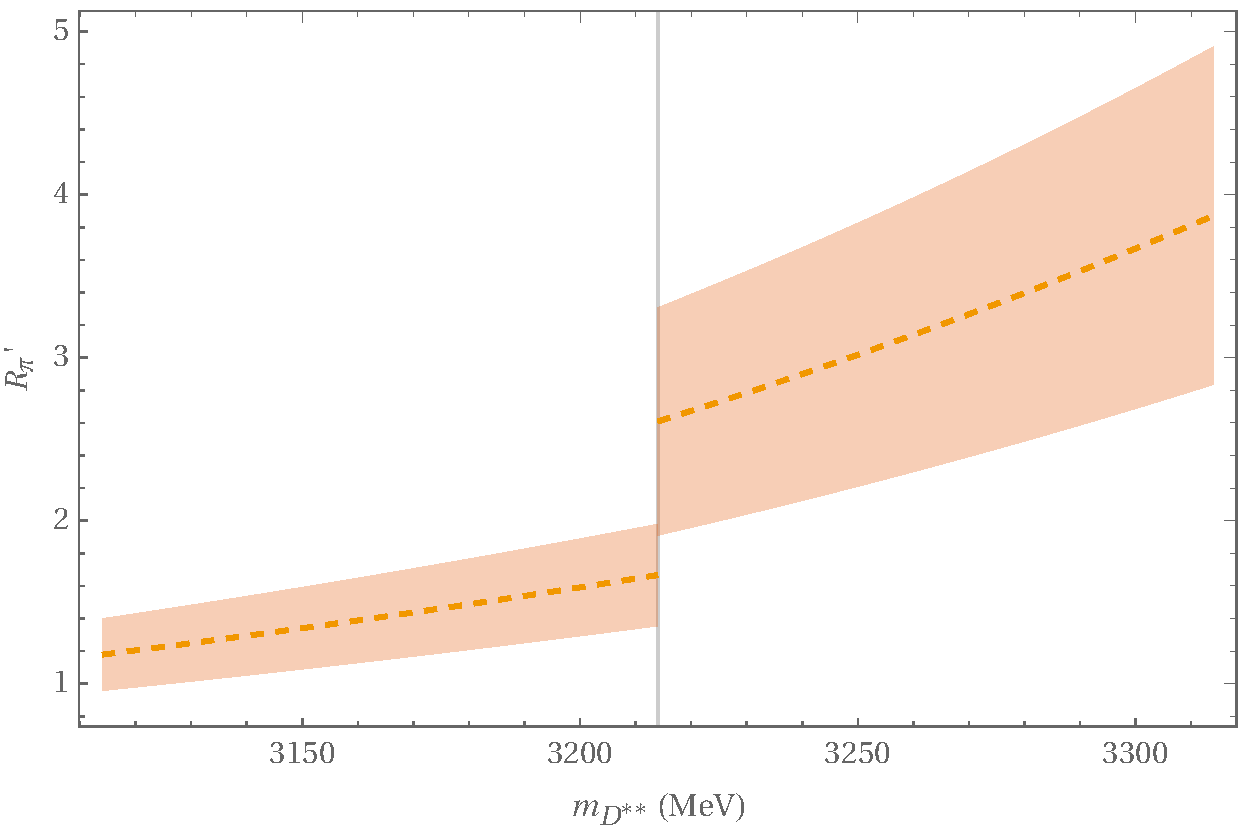
\includegraphics[width=0.8\textwidth]{figures/plot.pdf}
  \caption{Possible values of $R'_\pi$ against the mass of $D^{* \prime}_{s 2}$. The left-hand side refers to the case in which $D^*_2(3000)$ belongs to the $\tilde{T}$ doublet and $D^{**}$ is its spin partner with $J^P=1^+$. The right-hand side refers to the case in which $D_2^*(3000)$ belongs to the $F$ doublet and $D^{**}$ is its spin partner with $J^P=3^+$.}
  \label{fig:R'pi}
\end{figure}

Finally, the observation of the $D_2^*(3000)$ allows to draw further conclusions. Indeed, the strange partner of the $D^*_2(3000)$, namely the $D^{* \prime}_{s 2}$, should have mass of about $3.3 \ \text{GeV}$. This information can be used to calculate the analogous of equation \eqref{eq:Rpi_numeric} for decays of the $D^{* \prime}_{s 2}$ to a strange meson of the $H$ doublet plus $K$ or $\eta$. Such quantities are listed below, where I have assumed\footnotemark{} the value $3313 \pm 62 \ \text{MeV}$ for the mass of the $D^{* \prime}_{s 2}$
\footnotetext{It was used the following estimate
\begin{align*}
  m_{D^{* \prime}_{s 2}} &= m_{D^*_{s 2}(3000)} + \overline{\Delta m_s} \\
  \sigma \left( m_{D^{* \prime}_{s 2}} \right) &= \sqrt{\sigma \left( m_{D^{* \prime}_{s 2}(3000)} \right)^2 + \sigma \left( \Delta m_s \right)^2 }
\end{align*}
where $\overline{\Delta m_s}$ and $\sigma \left( \Delta m_s \right)$ are the weighted mean and standard deviation of the difference between the masses of $D$ mesons and their strange partner $m_s = m \left(D^{**}_s \right) - m \left( D^{**} \right)$, where $D^{**}$ are the $D(1869)$, the $D^*(2010)$, the $D^*(2600)$, the $D_1(2420)$, the $D^*_2(2460)$ and the $D^*_3(2760)$ (see table \ref{tab:charm_taxonomy}).}

\begin{subequations}
  \begin{align}
    R_K &= \frac{\Gamma \left( D_{s 2}^{* +} \rightarrow D^{* 0} K^+ \right) + \Gamma \left( D_{s 2}^{* +} \rightarrow D^{* +} K_S \right)}{\Gamma \left( D_{s 2}^{* +} \rightarrow D^0 K^+ \right) + \Gamma \left( D_{s 2}^{* +} \rightarrow D^+ K_S \right)} \ ,
    \quad
    R_K =
      \begin{cases}
        0.39 \pm 0.02 & F \\
        1.02 \pm 0.03 & \tilde{T} 
      \end{cases} \ , \\
    R_\eta &= \frac{\Gamma \left( D_{s 2}^{* +} \rightarrow D_s^+ \eta \right)}{\Gamma \left( D_{s 2}^{* +} \rightarrow D^0 K^+ \right) + \Gamma \left( D_{s 2}^{* +} \rightarrow D^+ K_S \right)} \ ,
  \quad
    R_\eta =
      \begin{cases}
        0.29 \pm 0.01 & F \\
        0.31 \pm 0.01 & \tilde{T} 
      \end{cases} \ , \\
    R^*_\eta &= \frac{\Gamma \left( D_{s 2}^{* +} \rightarrow D_s^{* +} \eta \right)}{\Gamma \left( D_{s 2}^{* +} \rightarrow D^0 K^+ \right) + \Gamma \left( D_{s 2}^{* +} \rightarrow D^+ K_S \right)} \ , 
   \quad 
    R^*_\eta =
      \begin{cases}
        0.10 \pm 0.01 & F \\
        0.29 \pm 0.02 & \tilde{T} 
      \end{cases} \ .
  \end{align}
  \label{eq:Rstrange}
\end{subequations}
It can be noticed that the most significant difference is found in the ratio $R_K$. Moreover, in the case $D^*_2(3000)$ belongs to the $F$ doublet the ratio $R_\eta^*$ is much smaller than $R_K$ and $R_\eta$, while in the event it belongs to the $\tilde{T}$ doublet the two ratios $R_\eta$ and $R_\eta^*$ are almost equal size and $R_K$ is much larger than the other two. These findings are summarized at the end of the chapter.

\section{Final remarks about $D_2^*(3000)$ decay modes}

The mass of $D^*_2(3000)$ is large enough to allow other decay modes besides those discussed in the previous section. For example, it can decay to members of doublets other than the $H$ doublet plus a light pseudoscalar meson. The features of such decay modes are different for the two assignments discussed in this thesis. One could argue that these modes are less important than the ones already considered, on the basis of the reduced phase space available for them. Moreover, their theoretical estimate would require the introduction of further coupling constants, at present unknown.

Other possible decay channels are those with the emission of a light vector meson, such as $D \rho$ or $D^* \rho$. In this case, the phase space would not be suppressed as in the case of decays to higher doublets and these modes cannot be neglected. Their estimate is possible using an approach similar to the one already exploited here. Indeed, an effective Lagrangian approach has been developed using the hidden gauge symmetry idea \cite{Bando:1985rf,Bando:1987br}. The description of this method is beyond the scope of this thesis. 

As a final remark, I would like to mention that, if the decay modes to $D\pi$ and $D^* \pi$ were the only relevant ones, it would have been possible to estimate the strong coupling constant appearing in the effective Lagrangian \eqref{eq:F_Lagrangian} in the two cases: by equating the theoretical expression of the decay widths to the experimentally measured total width one could have easily derived such a parameter and, consequently, it would have been possible to estimate the width of the spin partner. Due to the existence of the other decay modes mentioned above, this procedure could only lead to an upper bound on the strong coupling constant.

%I summarize below the main results that can allow to properly identify $D_2^*(3000)$.
\cleardoublepage
\vspace*{\fill}
\begin{center}
  \fbox{\begin{minipage}{\textwidth}
      {\Large \bfseries Summary of the Results for the Classification of the $D_2^*(3000)$} \\
    
    {\large \bfseries Case $D_2^*(3000)$ belongs to the $F$ doublet}
    \begin{itemize}
      \item Predicted ratio $R_\pi$ (defined in equation \eqref{eq:Rpi_formula}):
      \begin{equation*}
        R_\pi=0.40 \pm 0.01
      \end{equation*}
      \item Spin partner: $D_3^*$ with $J^P=3^+$. Should be looked for in the mass range $\approx 3.2\text{--}3.3 \ \text{GeV}$.
      \item Predicted  ratio $R_\pi^\prime$ defined in eq. (3.17):
      \begin{equation*}
        R_\pi^\prime=3.60 \pm 1.60
      \end{equation*}
      \item Predicted hierarchy for ratios $R_K,\ R_\eta, \ R_\eta^*$ for the strange partner (see equations \eqref{eq:Rstrange}):
      \begin{equation*}
        R_K > R_\eta \gg R_\eta^*
      \end{equation*}
      and, in particular
      \begin{equation*}
        R_K=0.39 \pm 0.02.
      \end{equation*}
    \end{itemize}
    
    {\large \bfseries Case $D_2^*(3000)$ belongs to the $\tilde{T}$ doublet}
    \begin{itemize}
      \item Predicted ratio $R_\pi$ (defined in eq. (3.15)):
      \begin{equation*}
        R_\pi=1.06 \pm 0.03
      \end{equation*}
      \item Spin partner: $\tilde{D}_1$ with $J^P=1^+$. Should be looked for in the mass range $\approx 3.1\text{--}3.2 \ \text{GeV}$.
      \item Predicted  ratio $R_\pi^\prime$ defined in eq. (3.17):
        \begin{equation*}
          R_\pi^\prime=1.50 \pm 0.60
        \end{equation*}
      \item Predicted hierarchy for ratios $R_K,\ R_\eta,\ R_\eta^*$ for  the strange partner (see equations \eqref{eq:Rstrange}):
      \begin{equation*}
        R_K \gg \ R_\eta \approx R_\eta^*
      \end{equation*}
      and, in particular
      \begin{equation*}
        R_K=1.02 \pm 0.03.
      \end{equation*}
    \end{itemize}
  \end{minipage}}
\end{center}
\vspace*{\fill}

% vim: ft=tex nonumber wrap linebreak display+=lastline guifont=Inconsolata\ 20 spell spelllang=en_gb

\chapter{Conclusions}

Thanks to the $B$-factories and the LHCb experiment, there exist an ever growing availability of new data and hadronic spectroscopy is becoming a field of precision physics. The theoretical analysis of this data requires an approach deeply rooted in QCD. In the case of heavy-light hadrons, at present, one of the best options is the heavy chiral perturbation theory, which, unlike potential models, allows a model independent description of such states in the limit in which heavy quarks have infinite mass and light ones are massless. This theory is an established research tool and is today widely used in the discussion heavy-light hadronic systems.

At present, the states of the open-charm meson spectrum fit rather nicely the predictions of the heavy chiral perturbation theory, although the puzzle of the low mass of the strange $S$ doublet with $n = 1$ still needs to be clarified. 

%Also, several empirical mass relations have revealed themselves to be good heuristics in the discussion of the classification of states. These relations do not derive from this theory in a formal way, but in light of heavy chiral perturbation theory appears reasonable. Arguments based on them suggested that one between the $D^*_1(2680)$ and the $D^*_{s 1}(2860)$ could be a state with $n = 3$, which, if confirmed, would be the first state of this kind. However, it should be noticed that confirmation that the $D^*_1(2680)$ is really not the $D^*(2600)$ is needed in the first place. 

Classification is the first step in each science, because it allows to find patterns and indicates where to look for missing pieces. Prominent examples are the Mendeleev's table and the early quark model. In the case of heavy meson spectroscopy and in particular of open-charm spectroscopy, there are many vacancies in the classification of states and future observations will surely enrich our understanding. In particular, it would be interesting to observe the spin partner of the $D^*_{s 1}(2700)$ and in general other states with $n = 2$, indeed a glance at the table \ref{tab:charm_taxonomy} reveals that practically all radial excited states have uncertain classification. These and other considerations show how the heavy-meson spectroscopy is still a young and promising field of research.

The case of $D^*_2(3000)$ was considered in some detail and original results, based on the formalism treated in this thesis, have been presented. This meson has been observed by LHCb Collaboration in 2016, and its spin parity has been fixed to $J^P=2^+$. Considering  the classification scheme discussed in this thesis, I have found that there are  two possible identifications for it. In order to distinguish between the two, several strategies have been proposed in this thesis. 

In particular, the first one relies on the calculation of the ratio of the branching fractions of the $D^*_2(3000)$ in $D \pi$ and $D^* \pi$. This quantity is sensitive to the quantum numbers of $D^*_2(3000)$ and hence suitable to classify it. This result is interesting in light of the upcoming measurements of the LHCb collaboration.

Other original results presented in this thesis are the predictions concerning the spin and the strange partners of the $D^*_2(3000)$. In particular, I have shown that exist a hierarchy among the possible decay modes of the latter that depends on the identification of the $D^*_2(3000)$. Hence, a measurement of such hierarchy could again provide a useful tool for the identification of this meson.

Finally, I would like to mention possible future investigations stemming from this work or connected to its theoretical framework. To begin with, within the heavy mesons spectroscopy, an interesting possibility is the determination of the low energy coupling constants of the heavy chiral perturbation theory from experimental data. This requires the evaluation of decay widths to final states with a light vector meson and involves extensions of the methods presented in this thesis. On the other hand, within the latter, it is possible to calculate decays to final states with an excited meson belonging to other doublets than the fundamental one plus a light pseudoscalar meson.

The spectroscopy of baryons containing a heavy quark, which as noticed in the first chapter is collecting new experimental achievements as well, can be studied using the same methods presented in this thesis. Indeed, once the covariant representation of baryon doublets is introduced, the decay widths of excited heavy baryons to a final state with a light pseudoscalar meson can be obtained from effective Lagrangians in a similar way.

% vim: ft=tex nonumber wrap linebreak display+=lastline guifont=Inconsolata\ 20 spell spelllang=en_gb

\newpage
\appendix
\chapter{Spinor Degrees of Freedom and Projectors}

Throughout this thesis several algebraic properties of spinors have been exploited. Given their relevance, some general remarks are recollected and presented in a systematic way in this appendix (the approach of which is taken from \cite{Steane:2013wra}).

A rank 1 spinor (or Weyl spinor or simply spinor) is a two component complex vector with defined Lorentz transformation law. Spinors can belong to two different representations of the Lorentz group $SO(3,1)$, which is homomorphic to $SL(2,\symbb{C})$, i.e. the group of $2 \times 2$ unimodular matrices, which are indicated in the literature as $(1/2, 0)$ and $(0, 1/2)$. The members of the first representation are called contraspinors or right-handed while the member of the second are called cospinors or left-handed.

The transformations of these two representations are the following
\begin{align}
  \operatorname{D}_R \colon u \mapsto \exp{\left( \frac{i}{2} (\symbf{\theta} + i \symbf{\rho}) \cdot \symbf{\sigma}\right)} u & \qquad \text{for contraspinors} \\
  \label{eq:contraspinor_transformation}
  \operatorname{D}_L \colon v \mapsto \exp{\left( \frac{i}{2} (\symbf{\theta} - i \symbf{\rho}) \cdot \symbf{\sigma}\right)} v & \qquad \text{for cospinors} ,
\end{align}
where $(\theta^i, \rho^i)$ are the parameters of the transformation (respectively the rotation angles and the rapidity vector components) and $\sigma^i$ are the Pauli matrices. Therefore, \emph{spinors of opposite chirality transform in the same way under pure rotations and in opposite way under pure boosts}. A Lorentz transformation for contraspinors is related to the transformation for cospinors with same parameters $\left( \operatorname{D}^\dagger_R \right)^{-1}$, in this way the contraction $v^\dagger u$ is Lorentz invariant (like the contractions of contravariant and covariant four-vectors).

The tensorial product of two rank 1 spinor is a rank 2 spinor, and so go on. Tensors of rank $k$ can be represented as spinors of rank $2k$. However, some tensors can be represented with spinors of the rame rank. This is shown explicitly for four-vectors in the following.

To begin with, notice that there is a linear isomorphism between four-vectors and Hermitian $2 \times 2$ matrices. The latter form a four-dimensional real vector space and a particularly convenient choice of a basis is $\{ \symbb{1}, \sigma^1, \sigma^2, \sigma^3 \}$
\begin{equation}
  X = 
  \begin{pmatrix}
    t + z & x - i y \\
    x + i y & t - z
  \end{pmatrix}
  = t \symbb{1} + x \sigma^1 + y \sigma^2 + z \sigma^3 = \sum_\mu x^\mu \sigma^\mu ,
\end{equation}
with $\sigma^\mu = (\symbb{1}, \symbf{\sigma})$. These matrices belong to a representation of the (complex two-dimensional) special linear group, if $M$ is Hermitian and $\operatorname{D}_{R/L}$ belongs to $SL(2, \symbb{C})$ then $\operatorname{D}_{R/L} M \operatorname{D}^\dagger_{R/L}$ is Hermitian, which is homomorphic to $SO(3,1)$ and indeed 
\begin{equation}
  \det{X} = t^2 - \left( x^2 + y^2 + z^2 \right) = x_\mu x^\mu ,
\end{equation}
\begin{equation}
  \det{\left( \operatorname{D}_{R/L}X \operatorname{D}^\dagger_{R/L}\right)} = \det X .
\end{equation}
The connection between the two groups is made apparent by the relations
\begin{subequations}
  \begin{align}
    \operatorname{D}^\dagger_R \sigma^\mu \operatorname{D}_R = \sum_\nu \Lambda\indices{^\mu_\nu} \sigma^\nu \\
    \operatorname{D}^\dagger_L \sigma^\mu \operatorname{D}_L = \sum_\nu \Lambda\indices{_\mu^\nu} \sigma^\nu 
  \end{align}
  \label{eq:sigma_sandwich}
\end{subequations}
where $\Lambda$ is the four-vector Lorentz transformations with same parameters.

At this point, it is sufficient to observe that the external product
\begin{equation}
  u u^\dagger = \begin{pmatrix} \vert a \vert^2 & a b^* \\ a^* b & \vert b \vert^2 \end{pmatrix} , \text{ with } u = \begin{pmatrix} a \\ b \end{pmatrix} ,
\end{equation}
is always a Hermitian null matrix which transforms covariatly with respect to Lorentz transformations, to conclude that a spinor is always associated to a null (or light-like) four-vector
\begin{equation}
  V = \frac{1}{2}
  \begin{pmatrix}
    \vert a \vert ^2 + \vert b \vert^2 \\
    a b^* + b a^* \\
    i ( a b^* - b a^* ) \\
    \vert a \vert^2 - \vert b \vert^2
  \end{pmatrix} = \frac{1}{2}
  \begin{pmatrix}
    u^\dagger u \\
    u^\dagger \symbf{\sigma} u 
  \end{pmatrix} .
\end{equation}
Moreover, it can be shown that any spinor can be uniquely represented by a tuple consisting of a light-like four-vector, a phase and a sign. 

Given a spinor, the associated four-vector can be extracted using the following relations 
\begin{align}
  V^\mu = u^\dagger \sigma^\mu u & \qquad \text{for contraspinors} \\
  \label{eq:fourvector_from_contraspinor}
  V_\mu = v^\dagger \sigma^\mu v & \qquad \text{for cospinors}. 
\end{align}
These light-like four-vectors can be interpreted as the four-velocity of massless particles. The number of available DoF's confirm this idea: in a given reference frame the four-velocity of a massless particle is determined by its direction (2 DoF's) while from a normalized Weyl spinor can be extracted a null four-vector with unitary time component (2 DoF's). 

Indeed, if $u$ is a spinor and $P$ is its four-vector then
\begin{align}
  \left(P^0 \symbb{1} - \symbf{P} \cdot \symbf{\sigma}\right) u = 0 & \qquad \text{for contraspinors} \\
  \left(P^0 \symbb{1} + \symbf{P} \cdot \symbf{\sigma}\right) v = 0 & \qquad \text{for cospinors} .
\end{align}
These equations can be interpreted as the \emph{Weyl equations} in the momentum space and describe massless spin-$1/2$ particles. For these particles the Pauli-Lubanski four-spin is proportional to the four-momentum: parallel in the case of right-handed solutions and anti-parallel in the case of left-handed solutions. For this reason, for Weyl particles, the helicity coincides with chirality. 

The Pauli-Lubanski four-spin is defined by
\begin{equation}
  W_\mu = \frac{1}{2} \varepsilon_{\mu \nu \alpha \beta} P^\nu J^{\alpha \beta} , 
\end{equation}
where $J^{\alpha \beta}$ is the relativistic angular momentum tensor (the charge of the Noether current of the Lorentz symmetry). This four-vector is the covariant generalization of the non relativistic spin, indeed it is proportional to the usual spin vector in the rest frame (which does not exist for Weyl particles, being massless)
\begin{equation}
  \left. W \right\vert_\text{rest frame} = \left( 0 , m \symbf{S} \right) 
\end{equation}
and, as such, is the generator of spin rotations. Moreover, as can be seen in the rest frame, it satisfies
\begin{equation}
  W_\mu W^\mu = - m^2 s ( s + 1 ) \qquad W_\mu P^\mu = 0 ,
\end{equation}
where $s$ is the spin of the field in exam. 

It is finally possible to transform a contraspinor in a cospinor and vice-versa, that is to find $\operatorname{P}$ such that
\begin{equation}
  \text{if } u \mapsto \operatorname{D}_Ru \text{ then } \operatorname{P} u \mapsto \left( \operatorname{D}^\dagger_R \right)^{-1} \operatorname{P} u .
\end{equation}
The interpretation of contraspinors and cospinors as solutions of the Weyl equation suggests that $\operatorname{P}$ is a spatial inversion. Indeed, the momentum $P^\mu$ is a polar vector while the Pauli-Lubanski four-spin $W^\mu$ is an axial one, therefore a spatial inversion transforms right-handed spinors into left-handed one and vice-versa. However, left-handed solutions of the Weyl equation correspond to negative frequency modes, that is to antiparticles. Therefore, in the case of Weyl particles, charge conjugation coincide with parity inversion. An explicit calculation shows that the form of $\operatorname{P}$ is
\begin{equation}
  \operatorname{P} \colon u \mapsto \begin{pmatrix} 0 & 1 \\ -1 & 0 \end{pmatrix} u^* .
\end{equation}

A bispinor (or Dirac spinor) is a vector with four complex components, thus eight real DoF's, transforming as a pair of spinors of opposite chirality. Conventionally, in the so-called chiral representation, the upper component is the right handed one, hence 
\begin{equation}
  \psi = \begin{pmatrix} u \\ v \end{pmatrix}, \qquad \operatorname{D}\colon \psi \mapsto 
  \begin{pmatrix}
    \operatorname{D}_R & 0 \\
    0 & \left( \operatorname{D}^\dagger_R \right)^{-1} 
  \end{pmatrix} \psi .
\end{equation}
The right and left-handed components of a bispinor can be projected by means of the \emph{chirality projectors}
\begin{equation}
  P_R = \frac{1 + \gamma^5}{2} \qquad P_L = \frac{1 - \gamma^5}{2} ,
\end{equation}
where $\gamma^5$ is the fifth gamma matrix, which in the chiral representation is 
\begin{equation}
  \gamma^5 = \begin{pmatrix} 1 & 0 \\ 0 & -1 \end{pmatrix} .
\end{equation}

A naive counting of the DoF's indicates that a normalized bispinor could represent an object with linearly independent four-momentum and four-spin. Because a bispinor transforms as a pair of spinors it is possible to extract two proper light-like four-vectors from them, in this way the available DoF's are reduced to five (where the normalization condition was taken into account). Notice that the two phases left out could be used to transform non trivially a bispinor without affecting its momentum or spin
\begin{subequations}
  \begin{align}
    U_R \colon \psi &\mapsto \begin{pmatrix} e^{i \alpha} & 0 \\ 0 & \symbb{1} \end{pmatrix} \psi \\
    U_L \colon \psi &\mapsto \begin{pmatrix} \symbb{1} & 0 \\ 0 & e^{i \alpha} \end{pmatrix} \psi .
  \end{align}
  \label{eq:u1_chiral_transformations}
\end{subequations}

To specify the state of a particle with spin, five parameters are sufficient indeed. This can be seen in two way. First: the four-momentum and the four-spin have 8 real parameters combined, 3 of which are fixed by the respective on-shell conditions and by the orthogonality condition. Second: to specify the state of such a particle is sufficient assign its velocity (3 DoF's) and the direction (and sign) of its spin (2 DoF's).

Let be $A^\mu$ and $B_\mu$ the two light-like four-vector associated with the right-handed and left-handed components of $\psi$
\begin{equation}
  A^\mu = u^\dagger \sigma^\mu u \qquad B_\mu = v^\dagger \sigma^\mu v ,
\end{equation}
then two orthogonal linear combinations can be formed
\begin{equation}
  V^\mu = A^\mu + B^\mu \qquad S_\mu = \frac{1}{2} \left( A_\mu - B_\mu \right),
\end{equation}
which can be written as
\begin{align}
  & V^\mu = u^\dagger \sigma^\mu u + \eta^{\mu \nu} v^\dagger \sigma^\nu v  = \psi^\dagger \gamma^0 \gamma^\mu \psi \\
  & S_\mu = \frac{1}{2} \left( \eta_{\mu \nu} u^\dagger \sigma^\nu u - v^\dagger \sigma^\mu v \right)  = \frac{1}{2} \psi^\dagger \gamma^0 \gamma_\mu \gamma^5 \psi ,
\end{align}
where all gamma matrices are in the chiral representation
\begin{equation}
  \gamma^0 = \begin{pmatrix} 0 & \symbb{1} \\ \symbb{1} & 0 \end{pmatrix} , \qquad \gamma^i = \begin{pmatrix} 0 & - \sigma^i \\ \sigma^i & 0 \end{pmatrix} .
\end{equation}

These two four-vectors are \textbf{not necessarily} non-null, however they have opposite invariant norm and hence if one is space-like the other is time-like and vice-versa. If in some particular frame of reference holds
\begin{equation}
  u = v \quad \text{ or } \quad u = - v 
  \label{eq:rest_frame_conditions}
\end{equation}
then $A^0 = B^0$ and $\symbf{A} = - \symbf{B}$. Therefore in this frame of reference $V^\mu$ and $S_\mu$ are suitable to be interpreted as the four-velocity and the four-spin of a particle at rest and the explicit expression of $\symbf{S}$ confirms this interpretation
\begin{equation}
  \symbf{S} = u^\dagger \symbf{\sigma} u .
\end{equation}
Once the equations for bispinorial fields are given, the two mutually exclusive possibilities \eqref{eq:rest_frame_conditions} are interpreted respectively as particles and antiparticles.

However, it is important to note that the conditions \eqref{eq:rest_frame_conditions} are \textbf{not} Lorentz covariant and so are referred to a particular frame of reference (if it exists). Nonetheless, in any given frame of reference, any bispinor can always be written as a sum of bispinors each satisfying respectively the first and the second of the equations \eqref{eq:rest_frame_conditions}
\begin{equation}
  \psi = \begin{pmatrix} u \\ v \end{pmatrix} \equiv \begin{pmatrix} (u + v)/2 \\ (u + v)/2 \end{pmatrix} + \begin{pmatrix} (u - v)/2 \\ (v - u)/2 \end{pmatrix} .
  \label{eq:rest_frame_decomposition}
\end{equation}
This decomposition can be obtained using the energy projectors, which in the given frame of reference have the form
\begin{equation}
  \operatorname{P}_+ = \frac{1 + \gamma^0}{2} \qquad \operatorname{P}_- = \frac{1 - \gamma^0}{2} .
  \label{eq:energy_projectors_rest}
\end{equation}
Moreover, if $\psi$ represent a particle (or an antiparticle) at rest in some other frame of reference, moving with speed $\symbf{v}$ with respect to the observer, then the decomposition \eqref{eq:rest_frame_decomposition} can be used in that frame and the result can be boosted with velocity $-\symbf{v}$
\begin{equation}
  \psi^\prime_\pm = \operatorname{D}(-\symbf{v}) \frac{1 \pm \gamma^0}{2} \psi = \frac{1 \pm \operatorname{D}(-\symbf{v}) \gamma^0 \operatorname{D}(\symbf{v})}{2} \psi' = \frac{1 \pm v_{0 \mu} \operatorname{D}(-\symbf{v}) \gamma^\mu \operatorname{D}(\symbf{v})}{2} \psi' = \frac{1 \pm \slashed{v}}{2} \psi' 
\end{equation}
where $v_0 = (1,\symbf{0})$, $\psi' = \operatorname{D}(-\symbf{v}) \psi$ and were taken into account the bispinorial analogous of the relations \eqref{eq:sigma_sandwich}
\begin{equation}
  \operatorname{D}(-\symbf{v}) \gamma^\mu \operatorname{D}(\symbf{v}) = \Lambda\indices{^\mu_\nu}(\symbf{v}) \; \gamma^\nu .
\end{equation}
In this way the generalized energy projectors are introduced
\begin{equation}
  \operatorname{P}_\pm = \frac{1 \pm \slashed{v}}{2} 
\end{equation}
and the bispinors projected using these operators have indeed the right velocity
\begin{equation}
  V^\mu = \psi_\pm \gamma^\mu \psi_\pm = \pm v^\mu .
\end{equation}

The same approach can be used to obtain the projectors for bispinor with spin in their rest frame parallel or antiparallel to $\symbf{s}$ in an arbitrary frame of reference
\begin{equation}
  P_{\uparrow \downarrow} = \frac{1 \pm \slashed{v} \slashed{s} \gamma^5}{2} , \quad \text{ with } s^\mu = \Lambda\indices{^\mu_\nu} \; s_0^\nu \text{ and } s_0^\mu = (0, \symbf{s})
\end{equation}
and verify that bispinors projected using the latter have the right spin 
\begin{equation}
  S^\mu = \frac{1}{2} \psi_{\uparrow \downarrow} \gamma^\mu \gamma^5 \psi_{\uparrow \downarrow} = \pm s^\mu .
\end{equation}

The interpretation of $V$ and $S$ as four-velocity and four-spin of the bispinor can be checked against another argument. If the operator which exchange the left and the right component
\begin{equation}
  \operatorname{P} \colon \psi \mapsto \begin{pmatrix} 0 & \symbb{1} \\ \symbb{1} & 0 \end{pmatrix} \psi = \gamma^0 \psi
\end{equation}
is interpreted as the spatial inversion (or parity transformation) operator then an explicit calculation show that $\symbf{V}$ change sign, i.e. is polar, while $\symbf{S}$ remain the same, i.e. is axial. This is the expected behaviour of the velocity and spin vectors. Moreover, as can be checked in the standard representation where $\operatorname{P}$ is diagonal, particle and antiparticle bispinors are eigenstates of the parity operator respectively with eigenvalues $+1$ and $-1$.

Finally, the bispinor charge conjugation operator can be introduced
\begin{equation}
  \operatorname{C} \colon \psi \mapsto \begin{pmatrix} 0 & \begin{pmatrix} 0 & -1 \\ 1 & 0 \end{pmatrix} \\ \begin{pmatrix} 0 & -1 \\ 1 & 0 \end{pmatrix} & 0 \end{pmatrix} \psi^*
\end{equation}
which simultaneously inverts the handedness of the two components and swap them. Its action is manifest in the rest frame, where it changes a particle bispinor in an antiparticle one and vice-versa.

% vim: spelllang=en_gb ft=tex

\backmatter
\pagestyle{plain}
\printbibliography
\chapter{Ringraziamenti}

\begin{otherlanguage}{italian}
Ammetto con franchezza---e non per cospargermi il capo di cenere---che la stesura di questa tesi sarebbe stata semplicemente impossibile senza l'aiuto ed il sostegno della mia relatrice, la dottoressa Fulvia De Fazio.

Se questo può dirsi vero per qualsiasi laureando, che, prescindendo dalla bontà della sua preparazione (o piuttosto delle sue intenzioni), arriva alla soglia della laurea, in ambiti ad altissima specializzazione, appena in grado di capire di cosa si parli---fatto nei cui confronti esiste, a voler chiamare le cose col proprio nome, un tabù---, nei confronti del proprio relatore; ebbene, nel mio caso, sento di dovere alla mia relatrice particolare gratitudine, da una parte, per l'aver sopportato senza spirito di rassegnazione le mie ostinate deficienze---nonchè, a volte, la mia deficente ostinazione (nel non darle ascolto)---, dall'altra, per aver profuso, nell'opera pia di traghettare il sottoscritto a questo traguardo, un impegno eccezionale e gratuito, ed infine per le cose che ho imparato.
\end{otherlanguage}

\end{document}

